\documentclass[a4paper]{article}
\usepackage{ fancyvrb, multicol}
\usepackage{ graphicx}

\usepackage[top=1.5 cm, bottom=2cm, left=1.5cm, right=1.5 cm]{geometry}
\begin{document}
\begin{center}
\vspace{3cm}
{\bf{\huge Chord book }}\\
\vspace{2cm}
{\bf Created for mre}\\\vspace{2cm}
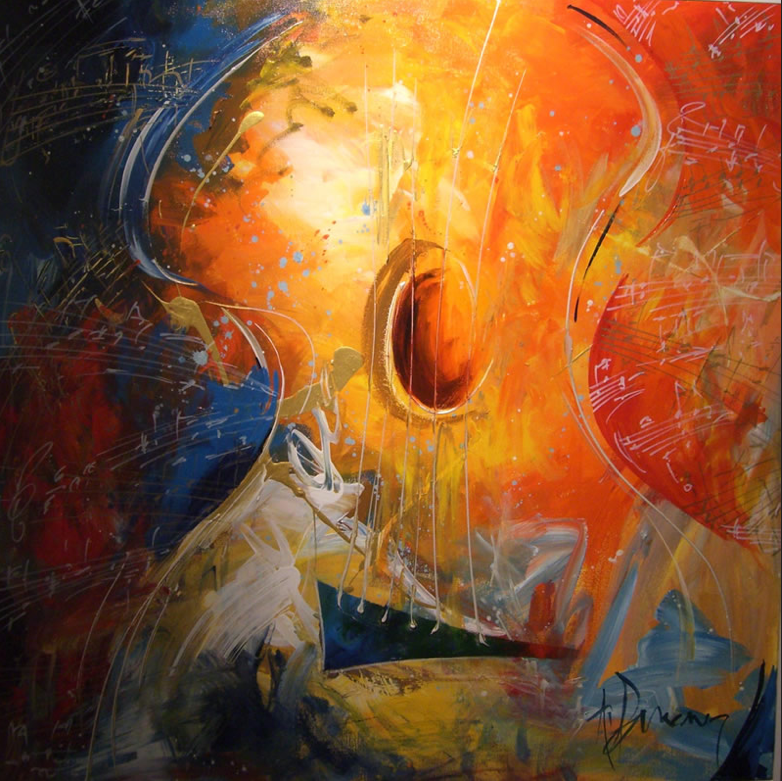
\includegraphics[scale=.6]{guitar2.png}\\
\vspace{1cm}
% \emph{A(nother) collection of all the songs I love to play}
\\
by Michele Esposito \\
\end{center}

\newpage
\tableofcontents
\newpage

\section{Buena Vista Social Club}
\subsection{Quizas, Quizas, Quizas}
\begin{Verbatim}[commandchars=\\\{\}]
{\bf (introducción en teclado)}
{\bf RE,MI,FA,MI,FA,RE, SOL, FA,MI,RE,MI,DO,}
{\bf RE,DO,SI,LA,SOL,LA,SI,DO,RE,}
{\bf RE,MI,FA,MI,FA,RE, SOL, FA,MI,RE,MI,DO,}
{\bf RE,DO,SI,LA,SOL,LA}

{\bf                    Em          Am              Em}
Siempre que te pregunto que ¿Cuándo? ¿Cómo? y ¿Dónde?
{\bf      Am            Em       F#7     B7      E7}
Tu siempre me respondes:  Quizás, quizás, quizás
{\bf                  Em    Am         Em     Am}
Y así pasan los días y yo desesperando y tú,
{\bf         Em        F#7      B7     E7}
tú contestando:  Quizás, quizás, quizás.
{\bf            B7                        E}
Estás perdiendo el tiempo pensando, pensando
{\bf                      B7                   E}
Por lo que tu más quieras hasta cuando, hasta cuando
{\bf                 Em     Am         Em     Am}
Y así pasan los días y yo desesperando y tú,
{\bf          Em        F#7      B7     E7}
tú contestando:  Quizás, quizás, quizás.

{\bf solo teclado (introducción)}

{\bf                    Em          Am              Em}
Siempre que te pregunto que ¿Cuándo? ¿Cómo? y ¿Dónde?
{\bf      Am            Em       F#7     B7      E7}
Tu siempre me respondes:  Quizás, quizás, quizás
{\bf                  Em    Am         Em     Am}
Y así pasan los días y yo desesperando y tú,
{\bf          Em        F#7      B7     E7}
tú contestando:  Quizás, quizás, quizás.
{\bf            B7                        E}
Estás perdiendo el tiempo pensando, pensando
{\bf                     B7                   E}
Por lo que tu más quieras hasta cuando, hasta cuando
{\bf                 Em     Am        Em       Am}
Y así pasan los días y yo desesperando y tú,
{\bf           Em        F#7      B7     E7}
tú contestando:  Quizás, quizás, quizás.
{\bf   F#7      B7     E7}
Quizás, quizás, quizás. [bis..(3)]

\end{Verbatim}
\newpage
\section{Calle 13}
\subsection{Muerte en Hawaii}
\begin{Verbatim}[commandchars=\\\{\}]

{\bf Intro: Eb}

{\bf Eb}
Yo he peliao con cocodrilos
{\bf                           Bb}
Me he balanceado sobre un hilo cargando más de 500 kilos
{\bf Cm }
Le he dao la vuelta al mundo en menos de un segundo
{\bf Ab                         Bb}
He cruzao 100 laberintos y nunca me confundo
{\bf Eb}
Respiro dentro y fuera del agua como las focas
{\bf G7}
Soy a prueba de fuego, agarro balas con la boca
{\bf Cm}
Mi creatividad vuela como los aviones
{\bf Ab                             Bb}
Puedo construir un cerebro sin leer las instrucciones


{\bf Ab                         Bb}
Hablo todos los idiomas de todos los abecedarios
{\bf Cm}
Tengo más vocabulario que cualquier diccionario
{\bf Ab                     Bb}
Tengo vista de águila, olfato de perro
{\bf Cm}
Puedo caminar descalzo sobre clavos de hierro
{\bf Ab}
Soy inmune a la muerte
{\bf Cm}
No necesito bendiciones porque siempre tengo buena suerte
{\bf Ab}
Ven conmigo a dar un paseo por el parque
{\bf              G7}
Porque tengo más cuentos que contarte que García Marqués


{\bf Eb}
Por ti, todo lo que hago lo hago por ti
{\bf                                   Cm}
Es que tú me sacas lo mejor de mí

Soy todo lo que soy
{\bf           Ab               Bb}
Porque tú eres todo lo que quiero (x2)


{\bf Eb}
Puedo brincar la cuerda con solo una pierna
{\bf     Bb}
Veo buen la oscuridad sin usar una linterna
{\bf Cm}
Cocino lo que quieras, yo soy todo un chef
{\bf       Ab          Bb}
Tengo sexo 24 - 7 todo el mes
{\bf Eb}
Puedo soplar las nubes grises pa que tengas un buen día
{\bf G7}
También se como comunicarme por telepatía
{\bf Cm}
Por ti, cruzo las fronteras sin visa
{\bf Ab                            Bb}
Y le saco una buena sonrisa a la Mona Lisa


{\bf Ab                       Bb}
Por ti, respiro antes de morirme
{\bf Cm}
Por ti voy a la Iglesia y escucho toda la misa sin dormirme
{\bf Ab                  Bb}
Sigo siendo el Rey, aunque no tenga reino
{\bf Cm}
Mi sudor huele a perfume y nunca me despeino
{\bf Ab                        Bb}
Se pelear todas las artes marciales
{\bf Cm}
También se como comunicarme con los animales
{\bf Ab}
Mientras más pasa el tiempo me veo más joven
{\bf                   G7}
Y esta canción la compuse sin escuchar como Beethoven

{\bf Eb}
Por ti, todo lo que hago lo hago por ti
{\bf                                   Cm}
Es que tú me sacas lo mejor de mí

Soy todo lo que soy
{\bf           Ab               Bb}
Porque tú eres todo lo que quiero (x2)

\end{Verbatim}
\newpage
\subsection{La Vuelta al Mundo}
\begin{Verbatim}[commandchars=\\\{\}]
{\bf Bb}
No me regalen mas libros
{\bf A7}
{\bf Por que no los leo }
{\bf Dm}
Lo que he aprendido es por que lo veo 
{\bf          Bb                  A7}
Mientras mas pasan los anos me contradigo cuando pienso 
{\bf Dm                     G}
El tiempo no me mueve yo me muevo con el tiempo 

Soy las ganas de vivir 
las ganas de cruzar 
las ganas de conocer lo que hay despues del mar 
yo espero que mi boca nunca se calle 
tambien espero que las turbinas de este avion nunca me fallen 
no tengo todo calculado ni mi vida resuelta 
solo tengo una sonrisa y espero una de vuelta
yo confio en el destino y en la marejada 
yo no creo en la iglesia pero creo en tu mirada 
tu eres el sol en mi cara cuando me levanta 
yo soy la vida que ya tengo tu eres la vida que me falta 
asi que agarra tu maleta el bulto los motetes 
el equipaje tu valija la mochila con todos tus juguetes y 

{\bf B....                   A7....            Dm....}
dame la mano y vamos a darle la vuelta al mundo darle la vuelta al mundo 
{\bf G....}
darle al vuelta al mundo 
{\bf B....                   A7....            Dm....}
dame la mano y vamos a darle la vuelta al mundo darle la vuelta al mundo 
{\bf G....}
darle al vuelta al mundo 

la renta el sueldo el trabajo en la oficina 
lo cambie por las estrellas y por huertos de harina 
me escape de la rutina para pilotear mi viaje 
por que el cubo en el que vivia se convirtio en paisaje 
yo era un objeto esperando a ser ceniza 
un dia decidi hacerle caso a la brisa 
a irme resbalando detras de tu camisa 
no me convencio nadie me convencio tu sonrisa 
y me fui tras de ti persiguiendo mi instinto 
si quieres cambio verdadero pues camina distinto 
voy a escaparme hasta la constelacion mas cercana la suerte es mi oxigeno tus ojos son mi ventana 
quiero correr por 7 lagos en un mismo dia 
sentir encima de mis muslos el clima de tus nalgas frias 
llegar al tope de la sierra abrazarme con las nubes 
sumergirme bajo el agua y ver como las burbujas suben y

dame la mano y vamos a darle la vuelta al mundo darle la vuelta al mundo darle al vuelta al mundo 
dame la mano y vamos a darle la vuelta al mundo darle la vuelta al mundo darle al vuelta al mundo

\end{Verbatim}
\newpage
\section{Renato Carosone}
\subsection{Tu Vuo' Fa' L'Americano}
\begin{Verbatim}[commandchars=\\\{\}]
{\bf Lam                         Rem   Mi7           Lam}
Puorte 'e cazune cu nu stemma arreto 
{\bf  Lam                      Rem  Mi7      Lam         }
Na cuppulella cu 'a visiera aizata 
{\bf Rem                                             Lam}
Passe scampanianno pe' Tuleto,
{\bf Si7                                                          Mi7                                          }
comm'a nu guappo, pe' te fá guardá! 
{\bf                                  Lam}
Tu vuo' fá ll'americano,
Siente a me chi t''o ffa fá?
mericano, 'mericano 
Tu vuoi vivere alla moda,
{\bf                                           Mi7}
po' te siente 'e disturbá 
ma se bevi "Whisky and Soda",
Tu abballe 'o "Rock and Roll",
{\bf                                        Lam}
tu giochi a "Base Ball "
{\bf                            Rem}
Ma 'e solde p''e Ccamel,
{\bf                        Lam}
{\bf chi te li dá?}
{\bf                       Si7}
La borsetta di mammá!?
{\bf                Mi7}
Tu vuó' fá ll'americano,
{\bf              Fa7                  Mi7}
mericano, mericano,
{\bf                                  Lam}
{\bf             La7       Rem}
ma si' nato in Italy!
{\bf                                                 Lam}
Siente a me: Nun ce sta niente 'a fá 
{\bf      Fa7     Mi7 Lam}
Okay, Napolitan!
{\bf                Mi7            Lam}
Tu vuó' fá ll'american!
{\bf                Mi7            Lam}
Tu vuó' fá ll'american!

Comme te pò capí chi te vò' bene,
si tu lle parle miezo americano?
Quanno se fa ll'ammore sott''a luna,
comme te vene 'ncapa 'e dí "I love you"?
Tu vuo' fá ll'americano,
mericano, 'mericano 
ma si' nato in Italy!
Siente a me: Nun ce sta niente 'a fá 
Okay, Napolitan!

Tu vuó' fá ll'american!
Tu vuó' fá ll'american!
Whisky and soda e rock and roll
Whisky and soda e rock and roll

\end{Verbatim}
\newpage
\section{Eva Cassidy}
\subsection{Somewhere Over The Rainbow}
\begin{Verbatim}[commandchars=\\\{\}]
{\bf Intro:   C  G Em Am D G}

{\bf G   G     Bm       Bm}
Somewhere over the rainbow
{\bf C   Cm     G    G7}
    Way up high
{\bf C       Cm   G           Em}
There's a    land that I heard of
{\bf Am        D    G   G}
Once in a lullaby


{\bf G   G     Bm       Bm}
Somewhere over the rainbow
{\bf C   Cm        G    G7}
    Skies are blue
{\bf C   Cm  G               Em      Am}
And the dreams that you dare to dream
{\bf        D       G    G}
Really do come true


{\bf G                   G}
Some day I'll wish upon a star
{\bf     C                 Cm             Em Em  Em}
And wake up where the clouds are far behind me
{\bf       G                  G}
Where troubles melt like lemondrops
{\bf  F#7           F#7}
Away above the chimney tops
{\bf        Bm    Bm     Am   D}
That's where you'll find me

{\bf G   G     Bm       Bm}
Somewhere over the rainbow
{\bf C   Cm        G    G7}
    Bluebirds fly
{\bf C     Cm  G        Em}
Birds fly over the rainbow
{\bf Am           D         G   G}
Why then, oh why can't I?

{\bf G                   G}
Some day I'll wish upon a star
{\bf     C                 Cm             Em Em  Em}
And wake up where the clouds are far behind me
{\bf       G                  G}
Where troubles melt like lemondrops
{\bf  F#7           F#7}
Away above the chimney tops
{\bf        Bm    Bm     Am   D}
That's where you'll find me

{\bf G   G     Bm       Bm}
Somewhere over the rainbow
{\bf C   Cm        G    G7}
    Bluebirds fly
{\bf C     Cm  G        Em}
Birds fly over the rainbow
{\bf Am           D         G   G}
Why then, oh why can't I?

{\bf   G             G7}
If happy little bluebirds fly
{\bf   C}
Beyond the rainbow
{\bf Am      D        G}
{\bf Why, oh why can't I?}

\end{Verbatim}
\newpage
\section{The Cat Empire}
\subsection{The Chariot}
\begin{multicols}{2}\begin{Verbatim}[commandchars=\\\{\}]
{\bf            Verse 1:}
{\bf Em                        G}
This is a song that came upon me one night 
{\bf           Am}
When the news it had been telling me 
{\bf        C                D}
About one more war and one more fight
{\bf       Em }
And 'aeh' I sighed but then
{\bf      G}
I thought about my friends
{\bf          Am}
Then I wrote this declaration
{\bf          C              D}
Just in case the world end
{\bf  }


{\bf            Verse 2:}
Our guns
{\bf Em             G}
 We shot them in the things we said
{\bf         Am}
Ah we didn't need no bullets 
{\bf          C            D}
Cos we rely on some words instead 
{\bf Em}
Kill someone in argument
{\bf G}
Outwit them with our brains 
{\bf           Am}
And we'd kill ourselves laughing
{\bf          C                D}
At the funny things we'd say 



{\bf            Verse 3:}
And bombs 
{\bf Em              G}
  We had them saved for special times
{\bf           Am}
When the crew would call a shakedown 
{\bf      C            D}
We break down a party landmine 
{\bf Em}
Women that so sexy 
{\bf         G}
They explode us with their looks 
{\bf          Am}
Ah we blowing up some speakers 
{\bf           C              D        }
Jumping round till the ground shook 



{\bf            Verse 4:}
And missiles
{\bf Em                   G}
   They were the roadtrips that we launched
{\bf        Am}
T-t-tripping across this island 
{\bf             C              D}
Starting missions at the break of dawn
{\bf  Em}
Yawn and smile say 
{\bf         G}
What direction shall we take? 
{\bf Am}
Somewhere where it warm and wet 
{\bf C                        D}
This be the route we'd always take and 



{\bf            Chorus:}
{\bf Am                      Em}
  Our weapons were our instruments 
{\bf G           D          C}
Made from timber and steel 
{\bf               Am}
We never yielded to conformity 
{\bf       Em}
But stood like kings 
{\bf         G}
In a chariot that's riding on a 
{\bf    D}
Record wheel 

{\bf             Verse 5:}
{\bf            Em}
And our airforce flying 
{\bf             G}
When the frisbee in the sky 
{\bf          Am}
Have a session while we're smoking
{\bf              C           D}
Now we're feeling extra high 
{\bf           Em }
And we'd sneak into a carpark
{\bf             G}
With the skaties on our back 
{\bf             Am}
And we're flying down the levels howling 
{\bf          C                D}
On the attack now on the attack



{\bf            Verse 6:}
And battles 
{\bf Em                   G}
  They happened in these dancehalls 
{\bf            Am}
See we'd rather fight with music
{\bf     C               D}
Choosing one the rhythm war
{\bf Em}
Battle at these shakedowns 
{\bf          G}
And we battle at these gigs 
{\bf         Am}
We do battle in our bedrooms 
{\bf             C                D}
Made some sweet love to the beat 



           Bridge:
{\bf            Em}
Then our allies grew 
{\bf      G}
Wherever we would roam 
{\bf         Am }
See whenever we're together 
{\bf         C             D}
Any stranger feel at home 
{\bf       Em}
In a way we are an army 
{\bf           G}
But this army not destruct 
{\bf       Am}
No instead we're doing simple things
{\bf        C             D}
Good loving find it run amuck 



{\bf            Verse 7:}
{\bf Em}
This be a declaration 
{\bf    G}
Written about my friends
{\bf         Am}
It's engraved into this song 
{\bf          C               D}
So they know I'm not forgetting them 
{\bf       Em}
See maybe if the world contained
{\bf  G}
More people like these 
{\bf           Am}
Then the news would not be telling me
{\bf        C                   D}
About all that warfare endlessly and

{\bf  Chorus:}

\end{Verbatim}
\end{multicols}\newpage
\subsection{The Lost Song}
\begin{Verbatim}[commandchars=\\\{\}]
{\bf Dm    Bb    F    Am7}
{\bf  }
the words go a little like this... 
{\bf  }
{\bf VERSE 1: }
{\bf     Dm                                        Bb }
Oh, I had nine lives but I lost all of them 
{\bf               F }
And I've been searching in the night  
{\bf                          Am7 (and so on)...       }
And I've been searching in the rain 
I tried to find them, but they disappeared 
They walked away, they dressed in black 
They left my side and all I say is 
That I wasted time when I looked for them 
For now I know that things gone past  
Are never to be found again 
No never, never again 
I had nine lives but lost all of them... 
{\bf  }
{\bf VERSE 2: }
I had a plan but never finished it 
And I've been searching for the thought 
And I've been searching in a haze  
I try all days, to remember it 
But now the blueprint in my mind has gone 
My mind forgot the colour of direction 
And my eyes they see the hands 
That could've built that could've constructed 
The empire in my mind 
The empire I'll never find 
I had a plan but that was where it ended....ended..... 
{\bf  }
Depending on what version you have, various sections get repeated...
I'm sure you can work it out.

\end{Verbatim}
\newpage
\subsection{The Wine Song}
\begin{Verbatim}[commandchars=\\\{\}]
{\bf INTRO}
(3/4 time)
{\bf | Dm | F+/C# | F | G/B | Bb | }
{\bf Dm/A | A7 | Dm |}

{\bf Dm        F+/C#    F        G/B}
Songs and melodies change and change
{\bf Bb}
And sway
{\bf          Dm/A           E7/Ab      A7}
But they still stay the same
{\bf Dm                F+/C#         G/C       G/B}
The songs that we sung when the dark days come
{\bf         Bb            Dm/A         A7          Dm}
Are the songs that we sung when we chased them away
{\bf Dm        F+/C#   F    G/B}
If I ever found a pot of gold
{\bf         Bb        Dm/A        E7/Ab         A7}
I'd buy bottles untold of the nectar of the vines
{\bf Dm           F+/C#      F           G/B}
I'm going to die with a twinkle in my eye
{\bf          Bb              Dm/A          A7            }
{\bf     Dm}
'cause I sung songs spun stories loved laughed and drank wine

{\bf Gm       Dm    A7   Dm}
Tomorrow is another day
{\bf Gm           Dm     A7       Dm}
The cats are out to play, to play
{\bf      Gm        Dm        A7       Dm}
That old rusty spaceship wants to sail
{\bf Gm       Dm    A7  Dm}
Into the milky way again
     Dm       Abdim   A7     | /A /B 
{\bf /C# |}
On a river of red red wine

[For this section, its really just the four chords written, but I included the bass 
notes as at the start when it is slow, those are very pronounced. But its just the chords 
with that Jewish Hora feel by alternating between the 5ths]

Dm   Dm/A (repeat)
{\bf Run...}
(let's have some)
Gm  Gm/D (repeat)
{\bf Fun...}
{\bf (we'll)}
Dm   Dm/A (repeat)
Drink...
(a toast to the)
A7   A7/E  (repeat)
{\bf Sun...}

{\bf [Same chords as verse 1]}

In summer the bushfires rage and rage
And rage
On such beautiful days
And we fight them with water that runs through the cracks
Water we're desperately trying to save
So I'll just live on wine and water my vines
And sleep on the wind with the fires right behind
And sing on the beaches and dance through the night
Oh we'll cry 'pass the wine, pass the wine, pass the wine'

{\bf Gm       Dm    A7   Dm}
Tomorrow is another day
{\bf Gm           Dm     A7       Dm}
The cats are out to play, to play
{\bf      Gm        Dm        A7       Dm}
That old rusty spaceship wants to sail
{\bf Gm       Dm    A7  Dm}
Into the milky way again
     Dm       Abdim   A7     | /A /B 
{\bf /C# |}
On a river of red red wine

[Again, same chords as before]

{\bf Run...}
(let's have some)
{\bf Fun...}
{\bf (we'll)}
Drink...
(a toast to the)
{\bf Sun...}

[Instrumental solo. This part is the same chords as the "run run run" section. The 
tricky part is the melody line, which I wont include, but if anyone actually wants it just 
contact me]

{\bf F         C         A7  Dm}
Oh what a beautiful day today!
{\bf Gm        F      C    F}
Today's a day to celebrate
{\bf F         C       A7        Dm}
Grab your bucket, grab your spade
{\bf Gm            F       C         F}
We're heading down to Half Moon Bay
{\bf F       C        A7     Dm}
I saw a plane go into a cloud
{\bf Gm            F         C           F}
I'm drunk I'm happy I'm singing and loud
{\bf F                  C         A7  Gm   A7  Bb}
                            [where the leading melody is C# D E D]
Two o'clock in the arvo, but hey that's allowed...
{\bf Gm                F         | C     C/E | F }
{\bf           A7 Dm}
I'm having a good time and of that I am proud

\end{Verbatim}
\newpage
\section{Dire Straits}
\subsection{Lions}
\begin{Verbatim}[commandchars=\\\{\}]
{\bf Intro:  Bm7  D  A  G   Bm7  D  A  G   Bm7  Bm7  Bm7  F# C9 (Stop) }
{\bf Bm7     D        A         G9 }
Red sun, go down way over dirty town 
{\bf Bm7             D             A       E9 }
Starlings are sweeping around crazy shoals 
{\bf Bm7         D                   A                          G9 }
Yes, and a girl is there, high heeling across the square 
{\bf Bm7                 D                          A              E9 }
The wind it blows around in her hair, and the flags upon the poles 
{\bf Em9 }
Waiting in the crowd to cross at the light 
{\bf                      G     F#m7          Bm7   F#m7   Bm7   F#   C9 }
She looks around to find a face she can like. 
{\bf Bm7          D           A                        G9 }
Church bell, clinging on, trying to get a crowd, Evensong 
{\bf Bm7                D        A              E9 }
Nobody cares to depend upon, the chime it plays 
{\bf Bm7                        D                   A                   G9 }
They're all in the station, praying for trains, the congregation's, late again 
{\bf Bm7                 D             A                E9 }
It's getting darker, all the time, these flagpole days 
{\bf Em9 }
Drunk old soldier he gives her a fright 
{\bf                  G      F#m7   Bm7   F#m7   Bm7   F#   C9 }
He's crazy lion howling for a fight. 
{\bf Bm7           D               A                    G9 }
Strap hanging, gunshot sound, door slamming on the, overground 
{\bf Bm7                D              A                 E9 }
The starlings are tough, but the lions are made of stone 
{\bf Bm7                   D          A                               G9 }
Her evening paper is horror torn, but there's hope later for, capricorns 
{\bf Bm7                       D           A              E9 }
Her lucky stars give her just enough, ... to get her home 
{\bf Em9 }
Then she's reading about a swing to the right 
{\bf                               G     F#m7   Bm7   F#m7   Bm7   F#   C9 }
But she's thinking about a stranger in the night 
{\bf G                       A    G                        A }
I'm thinking about the lions, I'm thinking about the lions 
{\bf G                     A       Bm7   F#m7    Bm7   F#m7    Bm7   F#m7    Bm7 }
A   fade out 
What happened to the lions, tonight       (tonight)    (tonight) 

\end{Verbatim}
\newpage
\subsection{Wild West End}
\begin{Verbatim}[commandchars=\\\{\}]
{\bf D                D            Em               G}
 Steppin' out to Angellucci's, for my coffee beans
{\bf D                 D      Em           G}
 checking out the movies, and the magazines
{\bf D             D          Em                         G}
 waitress she watches me, crossing from the Barocco bar
{\bf D              D     Em       G}
 I'm getting a pickup, for my steel guitar
{\bf            D           D   Em           G}
 I saw you walking out,      Shaftsbury Avenue
{\bf D          D                Em      G}
 excuse me talking, I wanna   marry you
{\bf D        D                        Em                  G}
 this is seventh heaven street to me, don't you be so proud
{\bf D                    D      Em       G}
 You're just another angel,   in the crowd. 

{\bf              D              D         Em        G}
	And I'm walking in the wild west end
{\bf      D              D         Em        G}
	Walking in the wild west end
{\bf      D                 D         Em        G     D/A G/C /C D/}
	Walking with your wild best friend


And my conductress on the number nineteen, she was a honey
pink toenails and hands all dirty with the money
greasy greasy greasy hair, easy smile
made me feel nineteen, for awhile
and I went down to Chinatown
in the backroom it's a man's world, all the money go down
Duck inside the doorway, gotta duck to eat
right now feels all right now, you and me we can't beat walking -

{\bf Chorus}

And a gogo, dancing girl, yes I saw her
the deejay, he say, here's Mandy for ya
I fell all right to see her, but she's paid to do that stuff
She's dancing high, I move on by, the close ups can get rough
when you're walking in the wild west end . . .

{\bf Chorus / Tag}

\end{Verbatim}
\newpage
\section{The Doors}
\subsection{My Wild Love}
\begin{Verbatim}[commandchars=\\\{\}]
my wild love went ridin'

she rode all the day
{\bf E5               Bm}
she wrote to the devil 
{\bf     Am           Bm  E5}
and asked him to pay
{\bf E5            Bm}
the devil was wiser
{\bf Am           Bm   E5}
it's time to repent 
{\bf E5              Bm }
he asked her to give back
{\bf Am            Bm  E5}
the money she spent
{\bf E5                Bm  }
my wild love went ridin'
{\bf Am              Bm E5}
she rode to the sea
{\bf E5             Bm}
she gathered together
{\bf      Am             Bm  E5}
some shells for her head
{\bf E5               Bm}
she rode and she rode on
{\bf Am             Bm   E5}
she rode for a while
{\bf E5                  Bm }
then stopped for an evenin'
{\bf Am               Bm  E5}
and lay her head down
{\bf E5             Bm}
she rode on to Christmas
{\bf Am              Bm  E5}
she rode to the farm
{\bf E5          Bm}
she rode to japan
{\bf     Am           Bm  E5}
and we entered a town
{\bf E5               Bm}
by this time the river 
{\bf Am              Bm    E5}
had changed one degree
{\bf E5            Bm }
she asked the people 
{\bf Am            Bm  E5}
to let her go free
{\bf E5              Bm}
my wild love is crazy
{\bf Am                 Bm  E5}
she screams like a bird
{\bf E5               Bm}
she moans like a cat
{\bf Am             Bm    E5}
when she wants to be heard
{\bf E5*          D5   Bm}
my wild love went ridin' 
{\bf Am              Bm  E5}
she rode for an hour
{\bf E5               Bm}
she rode and she rested
{\bf Am                Bm  E5  }
and then she rode on

ride, c'mon

{\bf e---------------------------------------------------------}
{\bf B---------------------------------------------------------}
{\bf G----------------------------------4p2-4-4-2-2---2-4------}
{\bf D----------------------------2-2-5-------------5-----2----}
{\bf A-------2p0-2-2-0-0---0-2---------------------------------}
{\bf E-0-0-3-------------3-----0-------------------------------}

{\bf E5: 022xxx}
{\bf Bm: x24432}
{\bf Am: x02210}
{\bf E5*: x799xx}
{\bf D5: x577xx}


\end{Verbatim}
\newpage
\section{Francesco De Gregori}
\subsection{Buffalo Bill}
\begin{Verbatim}[commandchars=\\\{\}]
{\bf Do}
Il paese era molto giovane i soldati a cavallo erano la sua difesa
il verde brillante della prateria dimostrava lampante l'esistenza di Dio
del Dio che progetta la frontiera e costruisce la ferrovia
{\bf                          Do}
a quel tempo io ero un ragazzo 
che giocava a ramino e fischiava alle donne
{\bf Fa  Do}
    credulone e romantico con due baffi da uomo
{\bf Rem                               Sol             }
se avessi potuto scegliere tra la vita e la morte, 
{\bf Lam              Sol }
tra la vita e la morte
{\bf                 Do      Lam Sol7 Do Lam Sol7 Do}
avrei scelto l'America.
{\bf Fa                       Do}
Tra bufalo e locomotiva, la differenza salta agli occhi
{\bf Re7 }
la locomotiva ha la strada segnata, 
{\bf Sol       Re7     Sol     Mim  Sol7 Fa}
il bufalo può scartare di lato e cadere
{\bf                    Do      Lam           Rem7           Sol7}
questo decise la sorte del bufalo, l'avvenire dei miei baffi
{\bf      Sol      Do   La7  Re}
e il mio mestiere.
{\bf                              Sol         Fa#m}
Ora ti voglio dire c'è chi uccide per rubare, 
{\bf Mim                    La }
e c'è chi uccide per amore
{\bf Sol       La            La7         Re   }
il cacciatore uccide sempre per giocare, 
{\bf Si7             Mim            La}
io uccidevo per essere il migliore
{\bf Re                            Sol           Fa#m}
mio padre guardiano di mucche mia madre una contadina
{\bf Mim                    La7}
io unico figlio biondo quasi come Gesù
{\bf Sol         La   Mim                 Re}
avevo pochi anni e vent'anni sembran pochi
{\bf Si7                                 Mim  La  Re  Re7}
poi ti volti a guardarli e non li trovi più.
{\bf Sol}
E mi ricordo infatti un pomeriggio triste
{\bf Re}
io con il mio amico culo di gomma famoso meccanico
{\bf Sol}
sul ciglio di una strada a contemplare l'America
{\bf Re}
diminuzione dei cavalli aumento dell'ottimismo
{\bf Mi7                                      }
mi si presentarono i miei cinquant'anni 
{\bf          La        Mi           La       La7      Sol }
e un contratto col circo Pace e Bene a girare l'Europa
{\bf      Re           Sim     Mim7         La7            Re}
e firmai, col mio nome firmai e il mio nome era Bufalo Bill
{\bf Sim  Re  Sim  Re}

\end{Verbatim}
\newpage
\subsection{La Donna Cannone}
\begin{Verbatim}[commandchars=\\\{\}]
{\bf Do}
Butterò questo mio enorme cuore tra le stelle un giorno,
{\bf    Do7+}
giuro che lo farò
{\bf         Solm6                                        La}
e oltre l'azzurro della tenda nell'azzurro io volerò.
{\bf Sol#                              Dom}
quando la donna cannone d'oro e d'argento dioventerà,
{\bf Sol}
senza passare dalla stazione
{\bf Sol7}
stazione l'ultimo treno prenderà.

{\bf Do}
E in faccia ai maligni e ai superbi
{\bf    Do7+              Solm6}
il mio nome scintillerà, dalle porte
{\bf La            Sol#}
della notte il giorno si bloccherà,

un applauso del pubblico pagante lo
{\bf Dom          Sol}
sottolineerà e dalla bocca del cannone
{\bf     Fa}
una canzone suonerà.


{\bf La                   Fa#m}
E con le mani amore, per le mani ti prenderò
{\bf   Sol}
e senza dire parole nel mio
{\bf Re}
cuore ti porterò
{\bf La         La7                    Fa#m}
e non aver paura se non sarò come bella come dici tu
{\bf Sol}
ma voleremo in cielo in carne ed ossa,
{\bf Sol7             Do}
non torneremo....Più,
{\bf     Do7  Lam  Do7 Solm4/7  Do7  Fa}
uuuh uuuh  uuuh  uuuh na na na na na

{\bf Fam                       Re}
E senza fame e senza sete e senza aria e senza rete
{\bf       Sol   Fa Sol Do}
voleremo via. 

{\bf Do                      Do7+}
Così la donna cannone, quell'enorme mistero volò,
{\bf Solm6                         La}
sola verso un cielo ner s'incamminò
{\bf Sol#                                  Dom}
Tutti chiusero gli occhi nell'attimo esatto in cui sparì,
{\bf Sol   Fa}
altri giurarono e spergiurarono che non erano rimasti lì.

{\bf La                   Fa#m}
E con le mani amore, per le mani ti prenderò
{\bf   Sol}
e senza dire parole nel mio
{\bf Re}
cuore ti porterò
{\bf La         La7                    Fa#m}
e non aver paura se non sarò come bella come dici tu
{\bf Sol}
ma voleremo in cielo in carne ed ossa,
{\bf Sol7             Do}
non torneremo....Più,
{\bf     Do7  Lam  Do7 Solm4/7  Do7  Fa}
uuuh uuuh  uuuh  uuuh na na na na na

{\bf Fam                       Re}
E senza fame e senza sete e senza aria e senza rete
{\bf       Sol   Fa Sol Do}
voleremo via. 

{\bf Do7  Lam  Do7 Solm4/7  Do7  Fa}

\end{Verbatim}
\newpage
\section{Gershwin}
\subsection{Summertime}
\begin{Verbatim}[commandchars=\\\{\}]
{\bf Em        Am7 Em       Am7       Em    Am7 Em}
Summertime,    and the livin' is easy
{\bf          Am7                       B7  C7 B7}
Fish are jumpin' and the cotton is high
{\bf              Em  Am7 Em       Am7          Em      Am7 Em}
Your daddy's rich,   and your momma's good lookin'
{\bf G                   A7 B7        Em  Am7 Em}
So hush little baby,   don't you cry

{\bf Em                   Am7 Em           Am7     Em      Am7 Em}
One of these mornings,   you're gonna rise up singing
{\bf             Am7                                      B7  C7 B7}
Then you'll spread your wings and you'll take to the sky
{\bf               Em     Am7 Em        Am7         Em       Am7 Em}
But till that morning,   there's a nothin' can harm you
{\bf      G              A7 B7       Em  Am7 Em}
With daddy and mammy   standing by

\end{Verbatim}
\newpage
\section{Grateful Death}
\subsection{Friend Of The Devil}
\begin{Verbatim}[commandchars=\\\{\}]
{\bf Intro:}
{\bf / G - - - / - - - - / C - - - / - - - - / x4}

{\bf G (2)}
I lit out from Reno,
{\bf             C (2)}
I was trailed by twenty hounds
{\bf  G (2)}
Didn't get to sleep that night
{\bf                C (2)}
'Till the morning came around.

{\bf Chorus:}
{\bf   D (2)}
Set out runnin' but I take my time
{\bf      Am (2)}
A friend of the devil is a friend of mine
{\bf    D (2)}
If I get home before daylight,
{\bf    Am (2)                                 D (4)}
I just might get some sleep tonight.

Ran into the devil, babe,
He loaned me twenty bills
I spent the night in Utah
In a cave up in the hills.

{\bf Chorus}

I ran down to the levee
But the devil caught me there
He took my twenty-dollar bill
And vanished in the air.

{\bf Chorus}

Bridge:
{\bf   D (2)}
Got two reasons why I cry
{\bf     D (2)}
Away each lonely night,
{\bf        C (2)}
The first one's named Sweet Anne Marie,
{\bf           C (2)                        }
And she's my hearts delight.
{\bf         D (2)}
The second one is prison, baby,
{\bf           D (2)}
{\bf The sheriff's on my trail,}
{\bf       Am (2)}
And if he catches up with me,
{\bf         C                    D (4)}
I'll spend my life in jail.

Got a wife in Chino, babe,
And one in Cherokee
The first one says she's got my child,
But it don't look like me.

{\bf Chorus}

{\bf Instrumental Verse & Chorus}

{\bf Repeat from Bridge, End at Chorus (hold last D)}

\end{Verbatim}
\newpage
\section{Jimi Hendrix}
\subsection{All Along the Watchtower}
\begin{Verbatim}[commandchars=\\\{\}]
{\bf 	  Am                G                F           G }
There must be some kind of way out of here
Said the joker to the thief
There's too much confusion
I can't get no relief
Buisness men they drink my wine
Plowmen dig my earth
None would ever compromise
Nobody of this world


No reason to get excited
The thief he kindly spoke
There are many here among us
Who feel that life is but a joke
But you and I we've been through that
And this is not our place
So let us stop talking falsely now
The hour's getting late


All along the watchtower
Princess kept the view
While all the women came and went
Barefoot servants too
Outside in the cold distance
A wildcat did growl
Two riders were approaching
And the wind began to howl


All along the watchtower
All along the watchtower
All along the watchtower

\end{Verbatim}
\newpage
\subsection{Bold as Love}
\begin{Verbatim}[commandchars=\\\{\}]
{\bf 	  A       E                     F#m                    D                    }
Anger!  He smiles towering in shiny metallic purple armor.   
{\bf D        A            E                     F#m                   D }
Queen Jealousy envy waits behind him, her firey green gown stares at the grassy ground.   
{\bf  D            A                              Bm                    G            }
Blue are the life-giving waters taken for granted, they quietly understand. 


{\bf D                      A                  Bm                    G    G6    }
Once happy turquoise armies lay opposite ready, but wonder why the fight is on. 
{\bf  A          E       F#m  G    }
But they're all bold as love. 
{\bf A            E        F#m   G        }
Yes they're all bold as love 
{\bf A         E           F#m  G  }
Yeah!  They're all bold as love. 
{\bf   }
{\bf  G            A            E                                          F#m }
Just ask the Axis...He knows ev'ry thing* 
{\bf A                E                           F#m                    D                    }
My red is so confident he flashes portraits of war, and visions of euphoria.   
{\bf A          E                      F#m                        D                    }
Orange is young, full of daring, but very unsteady for the first go round. 
{\bf A          E                                Bm      }
My yellow in this case is not so mellow, in fact I'm trying to say,  
{\bf           G }
It's frightened like me. 

{\bf  A                                E                         }
And all these emotions of mine keep pulling me from  
{\bf Bm                     G          A }
Giving my love to a rainbow like you, but I'm uh... 
{\bf   A          E       F#m  G    }
But they're all bold as love. 
{\bf A            E        F#m   G        }
Yes they're all bold as love 
{\bf A         E           F#m  G  }
Yeah!  They're all bold as love. 

{\bf  G            A   }
 Just ask the axis

\end{Verbatim}
\newpage
\subsection{Hey Joe}
\begin{Verbatim}[commandchars=\\\{\}]
{\bf 	  C       G  D      A                               }
  Hey Joe    where ya' goin' with that  
{\bf / E - - - / - - E7 - / E - - - / - - E7 - / }
gun in your hand? 
{\bf          C       G  D      A   }
I said, hey Joe      where ya goin' with that  
{\bf / E - - - / - - E7 - / E - - - / - - E7 - / }
gun in your hand?  

I'm goin' down to shoot my old lady.   I caught her messin' round with  
another man  
I'm goin' down to shoot my old lady.  You know I caught her messin' round with  
another man. 

Hey Joe,   I heard you shot your 
woman down you shot her down down 
Hey Joe,  I heard you shot your  
lady down, You shot her down to the ground 

Yes, I did, I shot her,  you know I caught her messin' 'round,  
messin' 'round town 
Yes, I did, I shot her,  you know I caught my old lady messin'  
'round the town, and I gave her the gun, I shot her 

 Guitar solo (3 Progressions) 

Hey Joe,where you gonna run to  
now, where you gonna run to? 
Hey Joe, I said, where you gonna  
run to now, Where you, where you gonna go? 

I'm goin' way down south, way down  
Mexico way, alright 

I'm goin' way down south, way down where  
I can be free--ain't no one gonna find me 

Ain't no hangman gonna, He ain't gonna put a rope around  
{\bf me}

Repeat Progression 
{\bf End on E }

\end{Verbatim}
\newpage
\subsection{The Wind Cries Mary}
\begin{Verbatim}[commandchars=\\\{\}]
{\bf  |:  Eb    E  F     Eb   E  F :| }
{\bf  }
{\bf C             Bb                 F }
After all the jacks are in their boxes 
{\bf C                   Bb          F }
And the clowns have all gone to bed 
{\bf C                      Bb            F }
You can hear happiness staggering on down the street 
{\bf G         Bb         Eb E F }
Footsteps dressed in red 
{\bf G       Bb            Eb E F  Eb E F }
And the wind whispers Mary 
{\bf  }
{\bf  }
{\bf C          Bb       F }
A broom is drearily sweeping 
{\bf C                       Bb          F }
Up the broken peices of yesterday's life 
{\bf C           Bb       F }
Somewhere a queen is weeping 
{\bf G           Bb          Eb E F }
Somewhere a king has no wife 
{\bf G            Bb    Eb E F  Eb E F }
And the wind cries Mary 
{\bf  }
{\bf  }
{\bf SOLO  |: F  Eb  Bb  Ab :| 3x    G  Bb  Db  F }
{\bf  }
{\bf  }
{\bf C                       Bb     F }
The traffic lights turn blue tomorrow 
{\bf C                       Bb         F }
And shine the emptyness down on my bed 
{\bf C               Bb   F }
The tiny island sags downstream 
{\bf G                   Bb       Eb E F }
Cause the life that lived is dead 
{\bf G            Bb      Eb E F  Eb E F }
And the wind screams Mary 
{\bf  }
{\bf  }
{\bf C             Bb     F }
Will the wind ever remember 
{\bf C                Bb           F }
The names it has blown in the past 
{\bf C                        Bb           F }
With its crutch, its old age, and its wisdom 
{\bf G                         Bb     Eb E F }
It whispers no, this will be the last 
{\bf G            Bb    Eb E F  Eb E F  Eb E F  Eb E F }
And the wind cries Mary 

\end{Verbatim}
\newpage
\section{Nuova Compagnia di Canto Popolare}
\subsection{Tammurriata Nera}
\begin{Verbatim}[commandchars=\\\{\}]
{\bf Lam                          Fa7                  Lam}
Io nun capisco, evvote, che succede 
{\bf                            Fa7}
e chello ca se vede,
{\bf                Lam}
nun se crede! nun se crede!
{\bf                            Fa7            Lam}
E' nato nu criaturo niro, niro 
{\bf                                                Fa7}
e 'a mamma 'o chiamma Giro,
{\bf          Lam           }
sissignore, 'o chiamma Giro 
{\bf La                 }
Seh! gira e vota, séh 
{\bf Sim}
Séh! vota e gira, séh 

{\bf                 Re                               La}
Ca tu 'o chiamme Ciccio o 'Ntuono,
{\bf                Fa#                            Sim}
ca tu 'o chiamme Peppe o Giro,
{\bf                Rem               La}
chillo, o fatto, è niro, niro,
{\bf                    Mi            La}
niro, niro comm'a che! 

'O contano 'e ccummare chist'affare:
"Sti fatte nun so' rare,
se ne contano a migliara!
A 'e vvote basta sulo na guardata,
e 'a femmena è restata,
sott'a botta, 'mpressiunata "
Seh! na guardata, seh 
Seh! na 'mpressione, seh 
Va' truvanno mo chi è stato
ch'ha cugliuto buono 'o tiro:
chillo, 'o fatto, è niro, niro,
niro, niro comm'a che! 
Ha ditto 'o parulano: "Embè parlammo,
pecché, si raggiunammo,
chistu fatto nce 'o spiegammo!
Addó' pastíne 'o ggrano, 'o ggrano cresce 
riesce o nun riesce,
sempe è grano chello ch'esce!"
Mé', dillo a mamma, mé' 
Mé', dillo pure a me 

Ca tu 'o chiamme Ciccio o 'Ntuono,
ca tu 'o chiamme Peppe o Giro,
chillo 'o ninno, è niro, niro,
niro, niro comm'a che! 

\end{Verbatim}
\newpage
\section{Peggy Lee}
\subsection{Tammurriata Nera}
\begin{Verbatim}[commandchars=\\\{\}]
{\bf Dm               Bb  A}
You had plenty money, 1922 
{\bf      Dm                  Bb        A}
You let other women make a fool of you 
{\bf               Gm                            Dm}
Why don't you do right, like some other men do? 
{\bf Gm         A    Bb              C#7    Dm   Bb A}
Get out of here and get me some money too 


You're sittin' there and wonderin' what it's all about 
You ain't got no money, they will put you out 
Why don't you do right, like some other men do? 
Get out of here and get me some money too 


If you had prepared twenty years ago 
You wouldn't be a-wanderin' from door to door 
Why don't you do right, like some other men do? 
Get out of here and get me some money too 


{\bf Dm Dm Bb A }
{\bf Dm Dm Bb A }
{\bf Gm Dm }
{\bf Gm A Bb C#7 }
{\bf Dm Dm Bb A}


I fell for your jivin' and I took you in 
Now all you got to offer me's a drink of gin 
Why don't you do right, like some other men do? 
Get out of here and get me some money too 
Why don't you do right, like some other men do? 
Like some other men do

\end{Verbatim}
\newpage
\section{Richie Havens}
\subsection{San Francisco Bay Blues}
\begin{Verbatim}[commandchars=\\\{\}]
{\bf F   D/F#  C    A    F   G   C   G }

{\bf G           C}
I got those blues where my baby 
{\bf         F                  C}
Left me down by the Frisco Bay, yea-yea
{\bf    F                              C}
An ocean liner came and took her away, yea-yea
{\bf   F                        }
I didn't mean to treat her bad,
{\bf              C                 A}
she was the best friend I ever had,
{\bf     D/F#         }
She said goodbye, she made me cry,
{\bf     G}
She made me wanna lay down my head and die...I 

Refrain:
{\bf C                        F                 C}
Ain't got a nickel and I ain't got a lousy dime
{\bf F                                             E}
She don't come back I think I'm gonna lose my mind
{\bf F                         D/F#          C                    A}
If she ever comes back to stay, 'sgonna be another brand new day
{\bf F                    G                    C           A}
Walkin' with my baby by the San Francisco Bay hey hey hey,
{\bf F                    G                    C      G}
Walkin' with my baby by the San Francisco Bay. 

{\bf  G           C        F     C}
Well I'm sittin' down on my back porch, 
{\bf C                  F      C}
I don't know which way to go
{\bf F                                            E}
The girl that I was so crazy about she don't love me anymore
{\bf F                       D/F#           C                 A}
Think I'm gonna catch a freight train, cause I'm feelin' blue
{\bf F                                     G}
Gonna ride it to the end of the line, thinkin' only of you! 

Refrain:

Kazoo-Solo
{\bf G           C}
(I got those blues where my baby )
{\bf         F                  C}
(Left me down by the Frisco Bay, yea-yea)
{\bf    F                              C}
(An ocean liner came and took her away, yea-yea)
{\bf   F                        }
(I didn't mean to treat her bad,)
{\bf              C                 A}
(she was the best friend I ever had,)
{\bf     D/F#         }
(She said goodbye, she made me cry,)
{\bf     G}
(She made me wanna lay down my head and die...I )
{\bf C                        F                 C}
(Ain't got a nickel and I ain't got a lousy dime)
{\bf F                                             E}
(She don't come back I think I'm gonna lose my mind)
{\bf F                         D/F#          C                    A}
(If she ever comes back to stay, 'sgonna be another brand new day)
{\bf F                    G                       C          }
(Walkin' with my baby by the San Francisco Bay. )


{\bf C                        F                 C}
Ain't got a nickel and I ain't got a lousy dime
{\bf F                                             E}
She don't come back I think I'm gonna lose my mind
{\bf F                         D/F#          C                    A}
If she ever comes back to stay, 'sgonna be another brand new day
{\bf F                    G                    C           A}
Walkin' with my baby by the San Francisco Bay hey hey hey,
{\bf F                    G                    C      A}
Walkin' with my baby by the San Francisco Bay. 
{\bf F                     G             C}
Walkin' with my baby, by the Frisco Bay!!!

\end{Verbatim}
\newpage
\section{Red Hot Chili Peppers}
\subsection{Dosed}
\begin{Verbatim}[commandchars=\\\{\}]

{\bf Intro (picked part, before/including when bass comes in)}
{\bf E-12-------12-------12-------12-------|-10-------10-----7-----7-------|-}
{\bf B-------12-------12-------12-------12-|-------10------8-----8------12-|-}
{\bf G----12-------12-------12-------12----|----11-------9------9----12----|-}
{\bf D-------------------------------------|-------------------------------|-}
{\bf A-------------------------------------|-------------------------------|-}
{\bf E-------------------------------------|-------------------------------|-}

Repeat twice

{\bf Verse}

{\bf C        D        Em}
I--- got dosed by you
Closer than most to you
What am I supposed to do
Take it away I never had it anyway
Take it away everything will be okay

{\bf C        D       Em}
In you a star is born
You cut a perfect form
Someone forever warm
{\bf Lay on lay on lay on lay on}
{\bf Lay on lay on lay on lay on}

{\bf Chorus 1}

{\bf G             D                  Em C}
Way up on the mountain where she died
All I ever wanted was your life
Deep inside the canyon I can't hide
All I ever wanted was your life

{\bf Verse}

{\bf C              D    Em}
Show love with no remorse
Climb onto your seahorse
This ride is right on course
This is the way I wanted it to be with you
This is the way I knew that it would be with you
{\bf Lay on lay on lay on lay on}
{\bf Lay on lay on lay on lay on}

{\bf Chorus 2}

{\bf G             D                  Em C}
Way up on the mountain where she died
All I ever wanted was your life
Deep inside the canyon I can't hide
G          D               Em/G (i think) ------ C2
All I ever wanted was your life

{\bf Verse- (it sounds good doing the picked part [from the beginning] here during this verse)}

I--- got dosed by you
Closer than most to you
What am I supposed to do
(resume chords if you want, this is when the drums start again and we get
background vocals, Flea resumes the normal bass line)
{\bf G              D            Em}
Take it away I never had it anyways
Take it away and everything will be okay

{\bf Chorus 1}

Last 4 chords of song-
{\bf C Em/G Am G}

\end{Verbatim}
\newpage
\subsection{I Could Die for You}
\begin{multicols}{2}\begin{Verbatim}[commandchars=\\\{\}]
{\bf 	  Intro. A   E  F#m }
{\bf  }
{\bf F#m                              C# }
Something inside the cards  
{\bf                          F#m }
I know is right  
{\bf  }
Don't want to live  
{\bf          C# }
Somebody elses life  
{\bf A }
This is what I want to be  
{\bf         Bm }
And this is what I give to you  
{\bf                             A }
Because I get it free  
{\bf                               Bm }
She smiles while I do my time  
{\bf  }
{\bf A          E        Bm   F#m }
I could die for you  
{\bf A          E           Bm      A   E }
Oh this life I choose  
{\bf  }
{\bf F#m                         C# }
I'm here to be your only go-between  
{\bf F#m                       C# }
To tell you of the sights  
{\bf                            A }
 Eyes have seen  
{\bf  }
What I really want to do is  
{\bf   Bm }
Turn it into motion  
{\bf                                 A }
Beauty that I can't abuse  
{\bf                               Bm }
You know that I'd use my senses to  
{\bf C# }
You can see that  
{\bf        D }
It's only everywhere  
{\bf C# }
I'd take it all and then  
{\bf        D }
I'd find a way to share  
{\bf  }
{\bf E }
Come along and go  
{\bf       D }
Along with me  
{\bf E }
Wander with me yo  
{\bf       D }
It's all for free  
{\bf  }
{\bf A         E           Bm    F#m }
I could die for you  
{\bf  }
Whatchu wanna do  
{\bf A          E           Bm }
Oh this life I choose (2x) 
{\bf  }
{\bf C# }
Come again and tell me  
{\bf  }
Where you want to go  
{\bf F#m }
What it means for me  
{\bf  }
To be with you alone  
{\bf C# }
Close the door and  
{\bf  }
No one has to know  
{\bf D             E }
{\bf How we are  }
{\bf  }
{\bf E }
Come along and go  
{\bf D }
Along with me  
{\bf E }
Wander with me yo  
{\bf D }
It's all for free  
{\bf  }
{\bf A          E         Bm   F#m }
I could die for you  
{\bf  }
What on want to do  
{\bf A          E          Bm }
Oh this life I choose  (4x) 

\end{Verbatim}
\end{multicols}\newpage
\subsection{Zephyr Song}
\begin{multicols}{2}\begin{Verbatim}[commandchars=\\\{\}]
{\bf 	  Intro: (Am G Em F) }
{\bf  }
{\bf Am                             }
 Can I get your hand and write on 
{\bf G  }
 Just a piece of leg and bite on 
{\bf Em }
 What a night to fly my kite on 
{\bf F }
 Do yoy want to flash light on 
{\bf Am                               G}
 Take a look it's on display...   for you 
{\bf Em                     F   }
 Coming down, no not today 

{\bf Am }
 Did you meet your fortune teller 
{\bf G }
 Get it off with no propeller 
{\bf Em }
 Do it up it's on with Stella 
{\bf F }
 What a way to finallu smell her 
{\bf Am                                  G }
 Pickin'up but not too strong...   for you 
{\bf Em                      F }
 Take a piece and pass it on 
{\bf }
{\bf Chorus:}
{\bf D }
 Fly away on my Zephyr 
{\bf G           A }
 I feel it more than ever 
{\bf D }
 And in this perfect weather 
{\bf G              A }
 We'll find a place together
{\bf }
{\bf  }
{\bf Am      G      Em     F }
Fly     on...  my    mind 
{\bf  }
{\bf Am }
 Rebel and liberator 
{\bf G }
 Find a way to be a skater 
{\bf Em }
 Rev it up to levitate her 
{\bf F }
 Super friendly aviator 
{\bf Am }
 Take a look it's on display 
{\bf G        Em                        F }
 For you...  comin' down no not today 
{\bf  }
{\bf Chorus }
{\bf  }
{\bf Am G Em F}
{\bf  }
{\bf Chorus}

\end{Verbatim}
\end{multicols}\newpage
\section{Simon and Garfunkel}
\subsection{A Poem On The Underground Wall}
\begin{Verbatim}[commandchars=\\\{\}]
{\bf Intro: C - C/B - G  -  G - G/F# - Em}


{\bf     C    C/B      G               G    G/F#      Em}
The last train is nearly due, the underground is closing soon,
{\bf     C      C/B    G               G       G/F#   Em}
And in the dark deserted station, restless in anticipation,
{\bf   C         C/B    G         G - G/F# - Em}
A man waits in the shadows.

{\bf  C        C/B  G                    G        G/F#     Em}
His restless eyes leap and scratch, at all that they can touch or catch,
{\bf     C      C/B      G              G      G/F#     Em}
And hidden deep within his pocket, safe within his silent socket,
{\bf    C       C/B      G        G - G/F# - Em}
He holds a coloured crayon.


{\bf     C        C/B      G               G        G/F#     Em}
Now from the tunnel's stony womb, the carriage rides to meet the groom,
{\bf     C     C/B      G                     G   G/F#   Em}
And opens wide and welcome doors, but he hesitates, then withdraws
{\bf  C     C/B    G         Em}
Deeper in the shadows.


{\bf         Em                         D}
And the train is gone suddenly, on wheels clicking silently
{\bf        C                 Am          Em               Am}
Like a gently tapping litany, and he holds his crayon rosary
{\bf  C             G       Em}
Tighter in his hand.


{\bf     C        C/B    G                     G     G/F#    Em}
Now from his pocket quick he flashes, the crayon on the wall he slashes,
{\bf  C    C/B     G              G      G/F#   Em}
Deep upon the advertising, a single-worded poem comprised of
{\bf  C  C/B  G      G - G/F# - Em}
Four letters.


{\bf         C         C/B      G       }
And his heart is laughing, screaming, pounding, 
{\bf     G    G/F#       Em}
The poem across the tracks rebounding,
{\bf  C       C/B    G               G         G/F#    Em}
Shadowed by the exit light, his legs take their ascending flight
{\bf    C        C/B       G        G/F#   C              G}
To seek the breast of darkness and be suckled by the night.

\end{Verbatim}
\newpage
\section{Steppenwolf}
\subsection{Magic Carpet Ride}
\begin{multicols}{2}\begin{Verbatim}[commandchars=\\\{\}]
{\bf D D     C   G G  D D   C   G G}
I like to dream, yes yees
Right between the sound machine
On a cloud of sound I drift in the night
Every place she goes is right
Flies far, flies near
To the stars away from here
{\bf  }
Well, you don't know what
We can find
Why don't you come with me little girl
On a magic carpet ride
{\bf  }
Well, you don't know, what
We can find
Why don't you tell your dreams to me
Fantasy will set you free
{\bf  }
{\bf CHORUS}
{\bf G}
Close your eyes girl
{\bf Bb}
Look inside girl
{\bf C                      G}
Let the sound take you away
{\bf  }
Last night I found Aladdin's lamp
So I wished that I could stay
But before the thing could answer me
Someone came and took the lamp away
{\bf  }
I looked
Around
A lousy candle's all I found
{\bf  }
Well, you don't know what
We can find
Why don't you come with me little girl
On a magic carpet ride
{\bf  }
Well, you don't know what
{\bf We can see}
Why don't you tell your dreams to me
Fantasy will set you free

\end{Verbatim}
\end{multicols}\newpage
\section{America}
\subsection{A Horse with No Name}
\begin{Verbatim}[commandchars=\\\{\}]
{\bf         Em                D6/9}
On the first part of the journey
I was lookin at all the life
There were plants and birds and rocks and things
There were sand and hills and rings

The first thing I met was a fly with a buzz
and the sky with no clouds
the heat was hot and the ground was dry
but the air was full of sound

{\bf  Chorus}

{\bf   Em9                              Dmaj9}
I've been through the desert on a horse with no name
it felt good to be out of the rain
in the desert you can remember your name
'cause there ain't no one for to give you no pain
la la la  la lalala   la la  la  la la


After two days in the desert sun
my skin began to turn red
After three days in the desert fun
I was looking at a river bed
And the story it told of a river that flowed
made me sad to think it was dead

{\bf  Chorus}

After nine days I let the horse run free
'cause the desert had turned to sea
there were plants and birds and rocks and things
there were sand and hills and rings
The ocean is a desert with it's life underground
and the perfect disguise above
Under the cities lies a heart made of ground
but the humans will give no love

\end{Verbatim}
\newpage
\section{Louis Armstrong}
\subsection{What a Wonderful World}
\begin{Verbatim}[commandchars=\\\{\}]
{\bf       G         Bm     C          Bm}
I see trees of green, red roses too
{\bf  Am7        G      B7         Em}
I see them bloom, for me and you,
{\bf       Eb               Am7     D7        G     / G7+5 / Cmaj7 / D7 /}
And I think to myself, What a  wonderful world.

I see skies of blue and clouds of white,
The bright blessed day, the dark sacred night,
{\bf                                                 C G}
And I think to myself, what a wonderful world

{\bf     D7                        G}
The colors of the rainbow, so pretty in the sky
{\bf     D7                   G}
Are also on the faces of people goin' by
{\bf       Em              D               Em         D}
I see friends shaking hands, saying, "How do you do?"
{\bf  Em             G#o       Am7  G#o    D7     C7}
They're really saying,  "I   love    you."       I hear

{\bf  (back to verse chords)}

Babies cry, I watch them grow
They'll learn much more than I'll ever know,
And I think to myself what a wonderful world(F / Am7b5 / )

{\bf        Am7             D7-9             G         C6  G6}
Yes I think to myself, what a wonderful world.

\end{Verbatim}
\newpage
\section{The Animals}
\subsection{House of the Rising Sun}
\begin{multicols}{2}\begin{Verbatim}[commandchars=\\\{\}]
{\bf   Am         C        D     F }
There is a house in New Orleans, 
{\bf  Am            C      E }
They call the Rising Sun 
{\bf      Am            C       D           F }
And It's been the ruin of many a poor boy 
{\bf  Am         E         Am    C D F Am E Am E }
And God, I know, I'm one 
{\bf   }
{\bf  Am        C     D     F }
My mother was a tailor 
{\bf  Am            C      E }
She sewed my new blue jeans 
{\bf      Am     C       D       F }
My father was a gambling man 
{\bf  Am         E   Am    C D F Am E Am E }
Down in New Orleans 
{\bf   }
{\bf  Am         C        D     F }
And the only things a gambler needs 
{\bf  Am            C      E }
Is a suitcase and a trunk 
{\bf      Am    C       D           F }
And the only time he's satisfied 
{\bf  Am         E         Am    C D F Am E Am E }
Is when he's all a-drunk 
{\bf   }
{\bf  Am         C        D     F }
I've got one foot on the platform 
{\bf  Am            C      E }
The other foot on the train 
{\bf      Am   C       D           F }
I'm going back to New Orleans 
{\bf  Am         E         Am    C D F Am E Am E }
To wear the ball and chain 
{\bf   }
{\bf  Am         C        D     F }
So mothers, tell your children 
{\bf  Am            C      E }
Not to do what I have done 
{\bf      Am   C       D           F }
Spend your life in sin and misery 
{\bf  Am         E         Am    C D F Am E Am E }
In the house of the Rising Sun 
{\bf   }
{\bf  Am         C        D     F }
There is a house in New Orleans, 
{\bf  Am            C      E    E }
They call the Rising Sun 
{\bf      Am            C       D           F }
And It's been the ruin of many a poor boy 
{\bf  Am         E         Am    C D F Am E Am E }
And God, I know, I'm one 

\end{Verbatim}
\end{multicols}\newpage
\section{Lucio Battisti}
\subsection{Un'Avventura}
\begin{multicols}{2}\begin{Verbatim}[commandchars=\\\{\}]
{\bf  Re Sol Re La }

{\bf  Re Sol Re }
Non sarà un'avventura 
{\bf  Fa#m Si7 }
non può essere soltanto una primavera 
{\bf  Mim La }
questo amore non è una stella 
{\bf  Sol La Sol La }
che al mattino se ne va. 
{\bf  Re }
Non sarà un'avventura 
{\bf  Fa#m Si7 }
questo amore è fatto solo di poesia 
{\bf  Mim La7 }
{\bf  tu sei mia, tu sei mia }
{\bf  Sol La }
fino a quando gli occhi miei 
{\bf  Sol La7 Re }
avran luce per guardare gli occhi tuoi. 


{\bf  Re Fa#m }
Innamorato sempre di più 
{\bf  Sol Re }
in fondo all'anima per sempre tu 
{\bf  Fa#m }
Perché non è una promessa ma è quel che sarà 
{\bf  Sol Re }
domani e sempre sempre vivrà, 
{\bf  La Re La }
sempre vivrà, sempre vivrà, sempre vivrà... 


{\bf  No, non sarà }
un'avventura 
non è un fuoco che col vento può morire 
ma vivrà 
quanto il mondo 
fino a quando gli occhi miei 
avran luce per guardare gli occhi tuoi. 

Innamorato sempre di più 
in fondo all`anima per sempre tu 
Perché non è una promessa ma è quel che sarà 
domani e sempre sempre vivrà, 
perché non è una promessa ma è quel che sarà

\end{Verbatim}
\end{multicols}\newpage
\subsection{Dieci Ragazze}
\begin{Verbatim}[commandchars=\\\{\}]
{\bf  Mi-                               }
Ho visto un uomo che moriva per amore, 
{\bf  Mi-                                      Do }
ne ho visto un altro che più lacrime non ha. 
{\bf          Mi-                 Do       }
Nessun coltello mai ti può ferir di più 
{\bf                                       Si }
di un grande amore che ti stringe il cuor. 

{\bf  Chorus}

{\bf  Mi- }
Dieci ragazze per me posson bastare 
{\bf  Mi-                             Sio }
dieci ragazze per me voglio dimenticare 
{\bf          Mi-             Sol }
capelli biondi da accarezzare 
{\bf          La                   DO }
e labbra rosse sulle quali morire. 
{\bf  Mi-                 Si7             Mi-   Mi-7  Mi-6  Do7+  Si }
Dieci ragazze per me     solo per me. 
{\bf  Mi-  }
Una la voglio perché sa bene ballare. 
{\bf  Mi-                                         Si7 }
Una la voglio perché ancor non sa cosa vuol dir l'amore. 
{\bf  Mi-              Sol       La                 DO }
Una soltanto perché ha conosciuto tutti tranne me. 
{\bf  Mi-             Si7                   Mi- }
Dieci ragazze così  che dicono solo di sì. 

{\bf  Si7                     Mi-               Re         Mi-   Re  Si7 }
Vorrei sapere chi ha detto   che non vivo più senza te. 
{\bf  Mi-                     Re        Sol            Si7 }
Matto, quello è proprio matto perché   forse non sa 
{\bf                    Mi-            Re     Mi-          Re   }
che posso averne una    per il giorno,  una per la sera 
{\bf             Mi-                                       Mi-   Si   }
però quel matto mi conosce perché ha detto una cosa vera. 
 

{\bf  Chorus}

{\bf  Si7                     Mi-               Re         Mi-   Re  Si7 }
Vorrei sapere chi ha detto   che non vivo più senza te. 
{\bf  Mi-                     Re        Sol            Si7 }
Matto, quello è proprio matto perché   forse non sa 
{\bf                    Mi-            Re     Mi-          Re   }
che posso averne una    per il giorno,  una per la sera 
{\bf             Mi-                                       Mi-   Si   }
però quel matto mi conosce perché ha detto una cosa vera. 
  


{\bf  Mi-                     Do                      La  }
Dieci ragazze per me    Dieci ragazze per me    Dieci ragazze per me 
 
{\bf  La                 Mi-   Do7                Mi-  }
però io muoio per te     però io muoio per te ..........

\end{Verbatim}
\newpage
\subsection{I Giardini di Maggio}
\begin{Verbatim}[commandchars=\\\{\}]
{\bf  Lam Mim7 Fa7+ Lam Mim7 Fa7+}

{\bf  Lam Mim7}
Il carretto passava e quell'uomo

{\bf  Fa7+}
gridava ”gelati”

{\bf  Lam Mim7}
al ventuno del mese i nostri soldi

{\bf  Fa7+}
erano già finiti

{\bf  Lam Mim7}
io pensavo a mia madre e rivedevo i

{\bf  Fa7+}
suoi vestiti

{\bf  Lam Mim7}
il più bello era nero coi fiori non

{\bf  Fa7+}
ancora appassiti

{\bf  Lam Mim7 Fa7+ Lam Mim7 Fa7+}

{\bf  Lam Mim7}
All'uscita di scuola i ragazzi

{\bf  Fa7+}
vendevano i libri

{\bf  Lam Mim7}
io restavo a guardarli cercando il

{\bf  Fa7+}
coraggio per imitarli

{\bf  Lam Mim7}
poi sconfitto tornavo a giocar con la

{\bf  Fa7+}
mente i suoi tarli

{\bf  Lam Mim7}
e la sera al telefono tu mi dicevi

{\bf  Fa7+ Sol Mim7}
perché non parli

{\bf  Do Sol}
Che anno è che giorno è questo è il

{\bf  Rem Mi7 Lam Lam7}
Tempo di vivere con te le mie mani come

{\bf  Rem}
vedi non tremano più

{\bf  Sol Mi7}
e ho nell'anima in fondo all'anima

{\bf  Do}
cieli immensi

{\bf  Sol Rem}
e immenso amore e poi ancora ancora

{\bf  Lam}
amore amor per te

{\bf  Lam7 Rem}
fiumi azzurri e colline e praterie dove

{\bf  Sol Mim7}
corrono dolcissime

{\bf  Lam Lam7}
le mie malinconie l'universo trova

{\bf  Rem}
spazio dentro me

{\bf  Lam Mim7 Fa7+}
ma il coraggio di vivere quello ancoranon c'è

{\bf  Lam Mi7 Fa7+ Lam Mim7 Fa7+}

{\bf  Lam Mim7}
I giardini di marzo si vestono di nuovi

{\bf  Fa7+}
colori

{\bf  Lam Mim7}
e le giovani donne in quel mese vivono

{\bf  Fa7+}
nuovi amori

{\bf  Lam Mim7}
camminavi al mio fianco e ad un tratto dicesti tu

{\bf  Fa7+ Lam Mim7 Fa7+}
Muori se mi aiuti son certa che io ne verrò fuori

{\bf  Lam Mim7 Fa7+}
ma non una parola chiarì i miei pensieri

{\bf  Lam Mim7 Fa7+ Sol Mi7}
continuai a camminare lasciandoti attrice di ieri

{\bf  Do Sol Rem}
Che anno è che giorno è questo è il tempo

{\bf  Mi7 Lam Lam7}
di vivere con te le mie mani come vedi non

{\bf  Rem}
tremano più

{\bf  Sol Mi7 Do}
e ho nell'anima in fondo all'anima
cieli immensi

{\bf  Sol Dom}
e immenso amore e poi ancora
ancora amore amor

{\bf  Lam Lam7 Rem}
per te fiumi azzurri e colline
e praterie dove

{\bf  Sol Mi7+}
corrono dolcissime

{\bf  Lam Lam7 Rem}
le mie malinconie l'universo trova spazio dentro me

{\bf  Lam Mim7 Fa7+}
ma il coraggio di vivere quello ancora non c'è

{\bf  Lam Mim7 Fa7+ Lam Mim7 Fa7+ Lam9}

\end{Verbatim}
\newpage
\subsection{Il Tempo di Morire}
\begin{multicols}{2}\begin{Verbatim}[commandchars=\\\{\}]
[C]  Moto[F]ci[C]cletta [F][C]
{\bf  10 [F]B[C]P [F][C]}
tutta [F]cro[C]mata [F][C]
{\bf  ? tua se [F]di[C]ci [G]s?   [C][G]}
mi cos[C]ta u[G]na [C]vita [F][C]
per niente [F]la [C]dar[F]ei   [Bb][F]
ma ho il cuo[Bb]re [F]ma[G]lato   [C][G]
{\bf  [F]  E so che [Bb]gua[F]ri[C]rei. [F][C]}

Non dire no
non dire no
non dire no
non dire no
lo so che ami un altro
ma che ci posso fare
io sono un disperato
perch? ti voglio amare.

Perch? ti voglio amare
perch? ti voglio amare
perch? ti voglio amare
stanotte, adesso, siiii?!
mi basta il tempo di morire
fra le tue braccia cos?
domani puoi dimenticare
ma adesso dimmi di s?.

Non dire no
non dire no
non dire no
prendi tutto quello che ho
mi basta il tempo di morire
fra le tue braccia cos?
domani puoi dimenticare
ma adesso dimmi di s?.

\end{Verbatim}
\end{multicols}\newpage
\section{The Beatles}
\subsection{Across the Universe}
\begin{Verbatim}[commandchars=\\\{\}]
{\bf  D                 Bm               F#m}
Words are flowing out like endless rain into a paper cup
{\bf        Em7                                    A                  A7}
{\bf  They slither while they pass they slip away across the Universe.}
{\bf  D                Bm               F#m}
Pools of sorrow, waves of joy are drifting through my opened mind
{\bf  Em7              Gm}
Possessing and caressing me.

{\bf  Chorus:}

{\bf  D             A7Sus4}
{\bf  Jai Guru Deva Om}
{\bf  A7			  }
Nothing's gonna change my world
{\bf  G			  D}
Nothing's gonna change my world
{\bf    A7			             }
Nothing's gonna change my world
{\bf        G			  D}
Nothing's gonna change my world


{\bf  D	  Bm		     F#m	   		    Em7}
Images of broken light which dance before me like a million eyes
{\bf        A		   A7}
{\bf  They call me on and on across the Universe.}
{\bf  D		 Bm		 F#m}
Thoughts meander like a restless wind inside a letterbox
{\bf       Em7			       A                 A7}
{\bf  They tumble blindly as they make their way across the Universe.}

{\bf  Chorus}

{\bf  D                   Bm			F#m}
Sounds of laughter, shades of earth are ringing through my opened ears
{\bf  Em7	     Gm}
Inciting and inviting me.
{\bf  D	     Bm		      F#m			      Em7}
Limitless, undying love which shines around me like a million suns
{\bf        A	     A7}
{\bf  And calls me on and on across the Universe.}

{\bf  Chorus x2}


\end{Verbatim}
\newpage
\subsection{All My Loving}
\begin{Verbatim}[commandchars=\\\{\}]
{\bf             Em            A7          D           Bm}
Close your eyes and I´ll kiss you, tomorrow i´ll miss you,
{\bf    G           Em        C     A7}
remember I´ll always be true.
{\bf           Em         A7             D         Bm}
And then while I´m away I´ll write home everyday
{\bf           G           A         D}
and I´ll send all my loving to you.
{\bf          Em            A7           D         Bm}
I´ll pretend that I´m kissing, the lips I am missing
{\bf      G            Em               C     A7}
and hope that my dreams will come true.
{\bf           Em         A7             D         Bm}
And then while I´m away I´ll write home everyday
{\bf           G           A         D}
and I´ll send all my loving to you.

{\bf         Bm     F#7            D}
All my loving I will send to you.
{\bf         Bm      F#7             D}
All my loving, darling I´ll be true.

{\bf             Em            A7          D           Bm}
Close your eyes and I´ll kiss you, tomorrow I´ll miss you,
{\bf    G           Em        C     A7}
remember I´ll always be true.
{\bf           Em         A7             D         Bm}
And then while I´m away I´ll write home everyday
{\bf           G           A         D}
and I´ll send all my loving to you.

{\bf         Bm     F#7               D}
All my loving I´ll will send to you.
{\bf         Bm      F#7             D}
All my loving, darling I´ll be true.

\end{Verbatim}
\newpage
\subsection{All You Need Is Love}
\begin{Verbatim}[commandchars=\\\{\}]
{\bf  G           D/F#      Em}
Love      love        love     
{\bf  G          D/F#     Em }
Love     love        love      
{\bf  D7/A    G          D7/A         }
Love     love       love

{\bf  G                                    D/F#                 Em}
There's nothing you can do that can't be done
{\bf  G                                   D/F#                    Em }
Theres nothing you can sing that can't be sung
{\bf  D7/A                   G                      D/F#                    }
Nothing you can say but you can learn to
{\bf                 D7/A}
play the game
{\bf  D7/A      D7}
It's          easy

There's nothing you can make that can't be made
No one  you can save that can't be saved
Nothing you can do but you can learn how to be you in time
It's easy

{\bf  CHORUS:}

{\bf  G          A7       D7}
All you need is love
{\bf  G          A7       D7}
All you need is love
{\bf  G          B7       Em         G/D }
All you need is love        love
{\bf  C             D7      G}
Love is all you need


There's nothing you can know that isn't known
Nothing you can see that isn't shown
Nowhere you can be that isn't where you're meant to be
Its easy

{\bf  CHORUS}

{\bf  C           D7      G}
Love is all you need   
{\bf  G          A7       D7}
All you need is love
{\bf  D7                         G          A7       D7}
All together now   All you need is love
{\bf  D7                        G          A7       D7}
Everybody now   All you need is love 

{\bf  G      D     G  }
Love is all you need   (repeats a few times)

\end{Verbatim}
\newpage
\subsection{Blackbird}
\begin{Verbatim}[commandchars=\\\{\}]
Blackbird singing in the dead of night 
Take these broken wings and learn to fly 
All your life You were only waiting for this moment to arise

Blackbird singing in the dead of night 
Take these sunken eyes and learn to see 
All your life 
You were only waiting for this moment to be free

Blackbird fly, blackbird fly 
Into the light of the dark black night
Blackbird fly, blackbird fly 
Into the light of the dark black night

Blackbird singing in the dead of night 
Take these broken wings and learn to fly 
All your life 
You were only waiting for this moment to arise 
You were only waiting for this moment to arise 
You were only waiting for this moment to arise 

\end{Verbatim}
\newpage
\subsection{Come Together}
\begin{Verbatim}[commandchars=\\\{\}]
{\bf  Dm}
Here come old flat top, He come grooving up slowly,
{\bf  Dm}
He got Joo Joo eyeball, He one holy roller 
{\bf  	A7		}
He got  Hair down to his knee;  
{\bf  G7}
Got to be a joker, he just do what he please.

{\bf            }
{\bf  			 (Riff)}
{\bf  Dm 			}
He wear no shoe shine, he got toe jam football
{\bf  Dm}
He got monkey finger, he shoot co-ca cola
{\bf          A7 }
He say, "I know you, you know me."  
{\bf  G7}
One thing I can tell you is you got to be free
{\bf       Bm              G}
Come Together, Right now, over me

{\bf  			 (Riff)}

{\bf  Dm}
He bag production, He got wal-rus gumboot
{\bf  Dm}
He got O-no sideboard, He one spinal cracker
{\bf         A7}
He got feet down below his knee
{\bf  G7}
Hold you in his armchair, you can feel his disease 
{\bf       Bm              G}
Come together, right now,  over me

{\bf  			 (Riff)}

{\bf  Dm}
He roller coaster, he got early warning
{\bf  Dm}
He got muddy water, He one Mo-jo filter
{\bf          A7}
He say, " One and one and one is three."
{\bf  G7}
Got to be good looking 'cause he so hard to see 
{\bf       Bm}
Come together, Right now, over me

\end{Verbatim}
\newpage
\subsection{I Am the Walrus}
\begin{Verbatim}[commandchars=\\\{\}]
{\bf  	  Intro:  B       A   G  F   E     E7     D     D7 }
{\bf       }
{\bf  A          A/G         C              D      E         A    A/G }
I am he as you are he as you are me and we are all together 
{\bf  C                                            D }
See how they run like pigs from a gun see how they fly 
{\bf      A }
I'm crying 
{\bf  A                    A/G    D/F#       Fmaj7         G          A  A/G }
Sitting on a cornflake                    waiting for the van to come 
{\bf  F }
Corporation tee shirt stupid bloody Tuesday man 
{\bf  B }
You've been a naughty boy you let your face grow long 


{\bf           C                       D                   E }
I am the eggman,   they are the eggmen,   I am the Walrus  Goo goo  g' joob
{\bf  }
{\bf   }

{\bf  A           A/G               C             D          E        A    A/G }
Mister city p'liceman sitting pretty little p'lice men in a row 
{\bf  C                                            D }
See how they fly like Lucy in the Sky see how they run 
{\bf        A                Dsus4      A            E     D   D7 }
I'm crying     I'm cry  ing  I'm crying   I'm cry  ing 

{\bf  A             A/G    D/F#        Fmaj7       G      A  A/G }
Yellow matter custard             dripping from a dead dog's eye 
{\bf  F }
Crab a locker fishwife pornographic priestess  
{\bf  B }
Boy you been a naughty girl you let your knickers down 

{\bf  }
{\bf           C                       D                   E }
I am the eggman,   they are the eggmen,   I am the Walrus  Goo goo  g' joob
{\bf  }
{\bf   }

Bridge:   E     B    A   G  F   E 

{\bf  B             A          G           F          E                }
Sitting in an English garden waiting for the sun.        
{\bf  F                                 B7  }
If the sun don't come you get a tan from standing in the English rain   

{\bf  Chorus: }
{\bf           C                       D                   E }
I am the eggman,   they are the eggmen,   I am the Walrus  Goo goo  g' joob  
Goo goo  g' joob            

{\bf  A          A/G           C              D      E         A    A/G }
Expert texpert choking smokers don't you think the joker laughs at you? 
{\bf  C                                            D }
See how they smile like pigs in a sty, see how they snied 
{\bf      A }
I'm crying 
{\bf  A             A/G    D/F#        Fmaj7       G      A  A/G }
Semolina pilchards                 climbing up the Eiffel Tower 
{\bf  F }
Element'ry penguin singing Hare Krishna.  
{\bf  B }
Man you should have seen them kicking Edgar Allan Poe 

{\bf           C                       D                   E }
I am the eggman,   they are the eggmen,   I am the Walrus  Goo goo  g' joob

\end{Verbatim}
\newpage
\subsection{I've Just Seen A Face}
\begin{Verbatim}[commandchars=\\\{\}]
{\bf  First verse:}
{\bf   G                                                                    Em}
I've just seen a face I can't for get the time or place where we just met
{\bf                                                                    C}
She's just the girl for me and I want all the world to see we've met
{\bf           D     G}
{\bf  Na na na na na na}


{\bf  Second verse:}
Had it been another day I might have looked the other way and
I'd have never been aware but as it is I'll dream of her tonight
{\bf  Da da da da da da }

{\bf  Chorus:}
{\bf     D                C                    G   C           G}
Falling yes I am falling and she keeps calling me back again

{\bf  Third verse:}
I have never known the likes of this I've been alone and I have 
Missed things and kept out of sight but as it is I'll dream of her tonight
{\bf  Da da da da da da }

{\bf  Repeat chorus.}

{\bf  Guitar solo played to verse chords.}

{\bf  Repeat chorus.}

{\bf  Repeat first verse.}

{\bf  Repeat chorus 3 times to end.}


\end{Verbatim}
\newpage
\subsection{Working Class Hero}
\begin{Verbatim}[commandchars=\\\{\}]
{\bf  Am                           G             Am}
As soon as you're born they make you feel small
{\bf                           G          Am}
By giving you no time instead of it all
{\bf                                       G       Am}
Till the pain is so big you feel nothing at all
{\bf      Am           (D)      G          Am}
A working class hero is something to be
{\bf      Am           (D)      G          Am}
A working class hero is something to be

They hurt you at home and they hit you at school
They hate you if you're clever and they despise a fool
Till you're so fucking crazy you can't follow their rules
A working class hero is something to be
A working class hero is something to be

When they've tortured and scared you for twenty odd years
Then they expect you to pick a career
When you can't really function you're so full of fear
A working class hero is something to be
A working class hero is something to be

Keep you doped with religion and sex and T.V.
And you think you're so clever and classless and free
But you're still fucking peasants as far as I can see
A working class hero is something to be
A working class hero is something to be

There's room at the top they are telling you still
But first you must learn how to smile as you kill
If you want to be like the folks on the hill
A working class hero is something to be
A working class hero is something to be

If you want to be a hero well just follow me
If you want to be a hero well just follow me

\end{Verbatim}
\newpage
\section{Patty Bravo}
\subsection{La Bambola}
\begin{multicols}{2}\begin{Verbatim}[commandchars=\\\{\}]
[Am]Tu mi fai girar
tu mi fai girar
come fossi una [E7]bambola
[Am]poi mi butti gi?
poi mi butti gi?
come [A7]fossi una [Dm]bambola
[E7]Non ti accorgi [Am]quando piango
[E7]quando sono [Am]triste e stanca [Dm6]tu
[E7]pensi solo per [Am]te[E7]

No ragazzo no
No ragazzo no
del mio amore non ridere
non ci gioco pi?
quando giochi tu
sai far male da piangere
Da stasera la mia vita
nelle mani di un ragazzo no,
[E7]non la lascer? [Am]pi?[C7]

{\bf {soc}}
[F]No ragazzo [Gm7]no
tu [C7]non mi mette[F]rai
tra le dieci [Gm]bambole
che [C7]non ti piacciono [F]pi?
{\bf  oh [E7]no, oh [Am]no[E]}

\end{Verbatim}
\end{multicols}\newpage
\section{Ray Charles}
\subsection{Hit the Road}
\begin{Verbatim}[commandchars=\\\{\}]
{\bf  Am	G	F	E}

(Hit the road Jack and don't you come back no more, no more, no more, no more.)
(Hit the road Jack and don't you come back no more.)
{\bf  What you say?}
(Hit the road Jack and don't you come back no more, no more, no more, no more.)
(Hit the road Jack and don't you come back no more.)

Woah Woman, oh woman, don't treat me so mean,
You're the meanest old woman that I've ever seen.
I guess if you say so
I have to pack ma things and go. (That's right)

(Hit the road Jack and don't you come back no more, no more, no more, no more.)
(Hit the road Jack and don't you come back no more.)
{\bf  What you say?}
(Hit the road Jack and don't you come back no more, no more, no more, no more.)
(Hit the road Jack and don't you come back no more.)

well baby, listen baby, don't ya treat me this-a way
Cause I'll be back on my feet some day.
(Don't care if you do 'cause it's understood)
(you ain't got no money you just ain't no good.)
Well, I guess if you say so
I'd have to pack my things and go. (That's right)

(Hit the road Jack and don't you come back no more, no more, no more, no more.)
(Hit the road Jack and don't you come back no more.)
{\bf  What you say?}
(Hit the road Jack and don't you come back no more, no more, no more, no more.)
(Hit the road Jack and don't you come back no more.)

well!!
(don't you come back no more.)
Uhh what did you say?
(don't you come back no more.)
i did not understand it
(don't you come back no more.)
i came to talk it over
(don't you come back no more.)
i thaught we had a better understanding
(don't you come back no more.)
oh baby dont be so chicken
(don't you come back no more.)
you dont want to see me cry x2
(don't you come back no more.)
oh baby it isnt fair
ooh yeahh

\end{Verbatim}
\newpage
\section{Eric Clapton}
\subsection{Wonderful Tonight}
\begin{Verbatim}[commandchars=\\\{\}]
{\bf  G   D/F#   C   D   G   D/F#   C   D}

{\bf  G                   D/F#}
   It's late in the evening
{\bf  C                         D}
   She's wondering what clothes to wear
{\bf  G                  D/F#}
   She puts on her make up
{\bf  C                   D}
   And brushes her long blonde hair
{\bf  C               D}
   And then she asks me
{\bf  G       Bm/F#   Em}
   Do I look alright
{\bf                C             D           G     D/F#  C  D}
   And I say yes, you look wonderful tonight


{\bf  G           D/F#}
   We go a party
{\bf  C                D}
   And everyone turns to see
{\bf  G                 D/F#}
   This beautiful lady
{\bf  C                   D}
   That's walking around with me
{\bf  C               D}
   And then she asks me
{\bf  G         Bm/F#   Em}
   Do you feel alright
{\bf                C           D           G}
   And I say yes, I feel wonderful tonight


{\bf             C}
   I feel wonderful
{\bf        D               G         Bm/F#   Em}
   Because I see the love light in your eyes
{\bf              C           D}
   And the wonder of it all
{\bf                  C             D}
   Is that you just don't realize
{\bf                 G        D/F#  C  D  G  D/F#  C  D}
   How much I love you


{\bf  G                   D/F#}
   It's time to go home now
{\bf  C                          D}
   And I've got an aching head
{\bf  G                     D/F#}
   So I give her the car keys
{\bf  C                   D}
   She helps me to bed
{\bf  C              D}
   And then I tell her
{\bf  G       Bm/F#         Em}
   As I turn out the light
{\bf               C                 D           G     Bm/F#  Em Em/D}
   I say my darling, you were wonderful tonight
{\bf            C                 D           G   D/F#  C  D  G  D/F#  C  D  G}
   Oh my darling, you were wonderful tonight

\end{Verbatim}
\newpage
\subsection{Layla}
\begin{Verbatim}[commandchars=\\\{\}]
{\bf  Intro:}
Dm   Bb   C   Dm (3 times) 
{\bf  Dm   Bb   C    A  C}


{\bf  C#m7                            G#7}
What will you do when you get lonely?
{\bf  C#m7           D              E  E7}
With no one waiting by your side
{\bf  F#m          B            E              A  }
You've been running and hiding much too long
{\bf  F#m            B                 E          A }
You know it's just your foolish pride    Layla

{\bf  Chorus}

{\bf  Dm   Bb       C            Dm}
         You got me on my knees Layla
{\bf  Dm   Bb        C               Dm}
         I'm begging darlin' please, Layla
{\bf  Dm   Bb    C                Dm}
         Darlin' won't you ease my worried mind
{\bf  Dm   Bb   C    A  C}


{\bf  C#m7                    G#7}
Tried to give you consolation,
{\bf  C#m7      D               E   E7}
Your old man had let you down
{\bf  F#m     B       E                 A  }
Like a fool, I fell in love with you,
{\bf  F#m              B                 E     A  }
You turned the whole world upside down Layla

{\bf  Chorus}


{\bf  C#m7                         G#7}
Let's make the best of the situation
{\bf  C#m       D           E  E7}
Before I fin'lly go insane
{\bf  F#m           B             E           A  }
Please don't say    we'll never find a way
{\bf  F#m          B               E      A  }
And tell me all my loves in vain  Layla
{\bf   }
{\bf  Chorus x2}

\end{Verbatim}
\newpage
\section{The Clash}
\subsection{London Calling}
\begin{Verbatim}[commandchars=\\\{\}]
{\bf  Em                     C}
London calling to the faraway towns
{\bf  G}
Now that war is declared-and battle come down
{\bf  Em                     C}
London calling to the underworld
{\bf  G}
Come out of the cupboard, all you boys and girls
{\bf  Em                  C}
London calling, now don't look at us
{\bf  G}
All that phoney beatlemania has bitten the dust
{\bf  Em                    C}
London calling, see we ain't got no swing
{\bf  G}
'cept for the ring of that truncheon thing


{\bf  Chorus}

{\bf  Em                       G}
The ice age is coming, the sun is zooming in
{\bf  Em                           G}
Engines stop running and the wheat is growing thin
{\bf  Em                         G}
A nuclear error, but I have no fear
{\bf  Em                       D                 Em}
London is drowning-and I live by the river



London calling to the imitation zone
Forget it, brother, an' go it alone
London calling upon the zombies of death
Quit holding out-and draw another breath
London calling-and I don't wanna shout
But when we were talking-i saw you nodding out
London calling, see we ain't got no highs
Except for that one with the yellowy eyes

{\bf  Chorus}

{\bf  For the outro just play the last line of the chorus.}

\end{Verbatim}
\newpage
\section{Leonard Cohen}
\subsection{Famous Blue Raincoat}
\begin{Verbatim}[commandchars=\\\{\}]
{\bf  Am                             F}
It's four in the morning, the end of December
{\bf      Dm7                     Em      }
I'm writing you now just to see if you're better
{\bf  Am                      F}
New York is cold, but I like where I'm living
{\bf          Dm7                     Em}
There's music on Clinton Street all through the evening.
{\bf  Am                 Bm                   Am   }
I hear that you're building your little house
{\bf                 Bm}
   deep in the desert
{\bf         Am         G           }
You're living for nothing now,
{\bf                   Am                   G}
   I hope you're keeping some kind of record

{\bf           C                                G}
Yes, and Jane came by with a lock of your hair
{\bf                               Am}
She said that you gave it to her
{\bf                                    Bm      G}
That night that you planned to go clear
{\bf  F               Em}
Did you ever go clear?

{\bf  Am                               F}
Ah, the last time we saw you you looked so much older
{\bf       Dm7                      Em}
Your famous blue raincoat was torn at the shoulder
{\bf  Am                           F}
You'd been to the station to meet every train
{\bf  Dm7                       Em}
And you came home without Lili Marlene


{\bf          Am         Bm         Am            Bm}
And you treated my woman to a flake of your life
{\bf      Am            G    Am               G}
And when she came back she was nobody's wife.


{\bf         C                                   G}
Well I see you there with the rose in your teeth
{\bf                      Am}
One more thin gypsy thief
{\bf                    Bm        G}
Well I see Jane's awake
{\bf  F             Em}
She sends her regards.

{\bf  Am                         F}
And what can I tell you my brother, my killer
{\bf  Dm7                 Em}
What can I possibly say?
{\bf  Am                         F}
I guess that I miss you, I guess I forgive you
{\bf  Dm7                      Em}
I'm glad you stood in my way.

{\bf  Am               Bm       Am          Bm}
If you ever come by here, for Jane or for me
{\bf  Am            G             Am           G}
Your enemy is sleeping, and his woman is free.

{\bf           C                           G}
Yes, and thanks, for the trouble you took from her eyes
{\bf                   Am                        Bm }
I thought it was there for good so I never tried.

{\bf      C                                G}
And Jane came by with a lock of your hair
{\bf                               Am}
She said that you gave it to her
{\bf                                    Bm       G}
That night that you planned to go clear
{\bf  F             Em}
Sincerely, L. Cohen

\end{Verbatim}
\newpage
\subsection{Master Song}
\begin{Verbatim}[commandchars=\\\{\}]
{\bf  G#			      Gm}
I believe that you heard your master sing 
{\bf  G#		   Gm}
when I was sick in bed. 
{\bf  G#			   Gm}
I suppose that he told you everything 
{\bf  G#			      Gm}
that I keep locked away in my head. 
{\bf  G#                   Cm}
Your master took you travelling, 
{\bf          Eb		      F}
well at least that's what you said. 
{\bf      Bb     Bb/A     Bb      Bb/A}
And now do you come back to bring 
{\bf       Eb		       D}
your prisoner wine and bread? 

{\bf  Intro x1}

You met him at some temple, where 
they take your clothes at the door. 
He was just a numberless man in a chair 
who'd just come back from the war. 
And you wrap up his tired face in your hair 
and he hands you the apple core. 
Then he touches your lips now so suddenly bare 
of all the kisses we put on some time before. 

And he gave you a German Shepherd to walk 
with a collar of leather and nails, 
and he never once made you explain or talk 
about all of the little details, 
such as who had a word and who had a rock, 
and who had you through the mails. 
Now your love is a secret all over the block, 
and it never stops not even when your master fails. 

And he took you up in his aeroplane, 
which he flew without any hands, 
and you cruised above the ribbons of rain 
that drove the crowd from the stands. 
Then he killed the lights in a lonely Lane 
and, an ape with angel glands, 
erased the final wisps of pain 
with the music of rubber bands. 

And now I hear your master sing, 
you kneel for him to come. 
His body is a golden string 
that your body is hanging from. 
His body is a golden string, 
my body has grown numb. 
Oh now you hear your master sing, 
your shirt is all undone. 

And will you kneel beside this bed 
that we polished so long ago, 
before your master chose instead 
to make my bed of snow? 
Your eyes are wild and your knuckles are red 
and you're speaking far too low. 
No I can't make out what your master said 
before he made you go. 

Then I think you're playing far too rough 
for a lady who's been to the moon; 
I've lain by this window long enough 
to get used to an empty room. 
And your love is some dust in an old man's cough 
who is tapping his foot to a tune, 
and your thighs are a ruin, you want too much, 
let's say you came back some time too soon. 

I loved your master perfectly 
I taught him all that he knew. 
He was starving in some deep mystery 
like a man who is sure what is true. 
And I sent you to him with my guarantee 
I could teach him something new, 
and I taught him how you would long for me 
no matter what he said no matter what you'd do. 

I believe that you heard your master sing 
while I was sick in bed, 
I'm sure that he told you everything 
I must keep locked away in my head. 
Your master took you travelling, 
well at least that's what you said, 
And now do you come back to bring 
your prisoner wine and bread? 

\end{Verbatim}
\newpage
\subsection{Suzanne}
\begin{Verbatim}[commandchars=\\\{\}]
{\bf     E               * +                      * +}
Suzanne takes you down to her place by the river
{\bf           F#m            * +                              *   +}
You can hear the boats go by, you can spend the night beside her
{\bf            E                    * +                            *    +}
And you know that she's half crazy but that's why you want to be there
{\bf           G#m                *  +             A                * +}
And she feeds you tea and oranges that come all the way from China
{\bf        E                                      F#m}
And just when you mean to tell her that you have no love to give her
{\bf            E}
Then she gets you on her wavelength
{\bf           F#m                                 E}
And she lets the river answer that you've always been her lover

{\bf           G#m}
And you want to travel with her
{\bf           A}
And you want to travel blind
{\bf            E}
And you know that she will trust you
{\bf               F#m                               E}
For you've touched her perfect body with your mind 

And Jesus was a sailor when He walked upon the water 
And He spent a long time watching from his lonely wooden tower
And when He knew for certain only drowning men could see Him 
He said, "All men will be sailors then until the sea shall free them"
But He Himself was broken long before the sky would open
Forsaken, almost human, He sank beneath your wisdom like a stone 

And you want to travel with him
And you want to travel blind
And you think maybe you'll trust him
For he's touched your perfect body with his mind 

Suzanne takes your hand, and she leads you to the river   
She is wearing rags and feathers from Salvation Army counters
And the sun pours down like honey on our lady of the harbor 
And she shows you where to look among the garbage and the flowers
There are heroes in the seaweed, there are children in the morning    
They are leaning out for love and they will lean that way forever   
while Suzanne holds the mirror 

And you want to travel with her
And you want to travel blind
And you know that you will trust her
For she's touched your perfect body with her mind

\end{Verbatim}
\newpage
\subsection{Teachers}
\begin{multicols}{2}\begin{Verbatim}[commandchars=\\\{\}]
{\bf  Intro: Am}

{\bf     Am          F}
I met a woman long ago
{\bf       Am                   F}
Her hair the black that black can go
{\bf       Am           F}
Are you a teacher of the heart?
{\bf   Am}
Soft she answered no

I met a girl across the sea
Her hair the gold that gold can be
Are you a teacher of the heart?
Yes, but not for thee

I met a man who lost his mind
In some lost place I had to find
Follow me the wise man said
But he walked behind

I walked into a hospital
Where none was sick and none was well
When at night the nurses left
I could not walk at all

Morning came and then came noon
Dinner time a scalpel blade
Lay beside my silver spoon

Some girls wander by mistake
Into the mess that scalpels make
Are you the teachers of my heart?
We teach old hearts to break

One morning I woke up alone
The hospital and the nurses gone
Have I carved enough my Lord?
Child, you are a bone

{\bf  I ate and ate and ate}
No I did not miss a plate, well
How much do these suppers cost?
We'll take it out in hate

I spent my hatred everyplace
On every work on every face
Someone gave me wishes
And I wished for an embrace

Several girls embraced me
Then I was embraced by men
Is my passion perfect?
No, do it once again

I was handsome, I was strong
I knew the words of every song
Did my singing please you?
No, the words you sang were wrong

Who is it whom I address
Who takes down what I confess?
Are you the teachers of my heart?
We teach old hearts to rest

Oh teachers are my lessons done?
I cannot do another one
They laughed and laughed and said, Well child
Are your lessons done?
Are your lessons done?
Are your lessons done?

\end{Verbatim}
\end{multicols}\newpage
\section{Elvis Costello}
\subsection{Almost Blue}
\begin{Verbatim}[commandchars=\\\{\}]
{\bf  Dm9    = 100210}
{\bf  E+     = XX2110}
{\bf  E7     = XX0100}
{\bf  Bm7-5  = 123231   (!!!!!!)}
Bflat6 = XX3333   (Bb6)
{\bf  Adim   = X02210}
{\bf  C#dim  = XX2323}

{\bf  INTRO:}
{\bf  Am     Dm9   E+}

{\bf  Am}
Almost blue
{\bf         Bm7-5 E7         Am}
Almost doing things we     used to do
{\bf            Bm7 -5               C            F}
There's a girl here and she's        almost you
{\bf  E       Dm}
      Almost
{\bf  Am      Adim}
All the things that your eyes once promised
{\bf  C       Bb6       A}
    I see in hers too
{\bf                    Dm       Bm7-5    E+}
Now your eyes are red from cry   -  ing

{\bf  Am    B7   Am}
    Almost blue

{\bf  F             Bm7-5           C       C#dim}
Flirting with this disaster became me
{\bf  Dm              Bm7-5           E}
    It named me as the fool who only aimed to be

{\bf  Am}
Almost blue
{\bf              Bm7-5    E7      Am}
It's almost touching it will     almost do
{\bf            Bm7-5             C          F    E     Dm}
There's a part of me that's     always true.....always
{\bf  Am                  Adim                     C          Bb6    A}
Not all good things come to an end now it is     only a chosen few
{\bf                 Dm         Bm7-5   E+}
I've seen such an unhappy cou  -  ple

{\bf  Am}
Almost me
{\bf  Bm7-5}
Almost you
{\bf         Am}
Almost blue

\end{Verbatim}
\newpage
\section{The Cranberries}
\subsection{Just My Imagination}
\begin{Verbatim}[commandchars=\\\{\}]
{\bf  Intro: A# F Cm Gm F}

{\bf  A#                          F}
There was a game we used to play
{\bf           Cm}
We would hit the town on Friday night
{\bf  Gm          F}
Stay in bed until Sunday
{\bf  A#               F}
We used to be so free
{\bf           Cm}
We were living for the love we had
{\bf  Gm             F}
Living not for reality

{\bf  CHORUS:}
{\bf  A#                   F}
Just my imagination, just my imagination
{\bf  Cm                Gm F}
Just imagination, it was
{\bf  A#                   F}
Just my imagination, just my imagination
{\bf  Cm                Gm F}
Just imagination, it was

{\bf  A#                         F}
There was a time I used to pray
{\bf         Cm}
I have always kept my faith in love
{\bf           Gm                      F}
It's the greatest thing from the man above
{\bf  A#                 F}
The game I used to play
{\bf              Cm}
I've always put my cards upon the table
{\bf  Gm                     F}
Never be said that I'd be unstable

{\bf  CHORUS}

{\bf  A#                        F}
There is a game I like to play
{\bf            Cm}
I like to hit the town on Friday night
{\bf  Gm          F}
Stay in bed until Sunday
{\bf  A#                   F}
We'll always be this free
{\bf             Cm}
We will be living for the love we have
{\bf  Gm             F}
Living not for reality

{\bf  A#                       F}
It's not my imagination, it’s not my imagination
{\bf  Cm                       Gm F}
It’s not my imagination, it was
{\bf  A#                  F}
Not my imagination, it’s not my imagination
{\bf  Cm                       Gm F}
It’s not my imagination, it was

{\bf  A#}
{\bf  Not my, not my...}

\end{Verbatim}
\newpage
\section{The Cream}
\subsection{White Room}
\begin{Verbatim}[commandchars=\\\{\}]
{\bf  Dm  C  Am  G}
{\bf  Ah  Ah Ah  Ah}

{\bf  Dm  C  Am  G  Em}
{\bf  Ah Ah  Ah  Ah Ah}

{\bf       Am        C            D      F G        Am     C  D F}
In a white room with black curtains near the stations

{\bf    G        Am    C          D       F  G     Am       C  D F}
Blackroof country, no gold pavements, tired starlings,

{\bf   G      Am   C          D       F G       Am       C  D F}
Silver horses run down moonbeams in your dark eyes.

{\bf   G         Am   C         D     F G      Am       C  D F}
Dawnlight smiles on your leaving, my contentment.

{\bf        G             D             F          E}
I'll wait in this place where the sun never shines.

{\bf   G            D                F      G            A      A}
Wait in this place where the shadows run from themselves.


You said no strings could secure you at the stations.
Platform ticket, restless diesels, goodbye windows.
I walked into such a sad time at the station.
As I walked out felt my own need just beginning.
I'll wait in the queue when the trains come back
I'll wait for you where the shadows run from themselves


At the party she was kindness in the hard crowd
Consolation from the old wound now forgotten
Yellow tigers crouched in jungles in her dark eyes
She's jst dressing goodbye windows, tired starlings
I'll sleep in this place with the lonely crowd,
Lie in the dark where the shadows run from themselves

{\bf                                     1  2  3  4   1  2  3  4}
{\bf  The main guitar riff is:  I Am    C    I D     F  G I}

\end{Verbatim}
\newpage
\section{Lucio Dalla}
\subsection{4 Marzo 1943}
\begin{Verbatim}[commandchars=\\\{\}]
{\bf  DO  LA-  DO}

{\bf       DO                                       SOL7}
Dice che era un bell'uomo e veniva, veniva dal mare
{\bf                                        DO}
parlava un'altra lingua, per• sapeva amare
{\bf                                                     SOL7}
e quel giorno lui prese a mia madre, sopra un bel prato
{\bf                                      DO      LA-  DO}
l'ora pi— dolce, prima d'essere ammazzato.
{\bf       DO                                         SOL7}
Cos lei rest• sola nella stanza, la stanza sul porto
{\bf                                       DO}
con l'unico vestito, ogni giorno pi— corto
{\bf                                             SOL7}
e benchŠ non sapesse il nome e neppure il paese
{\bf                                                  DO     LA-  DO}
mi aspett• come un dono d'amore, fino dal primo mese.
{\bf     DO                                   SOL7}
Compiva sedici anni, quel giorno la mia mamma
{\bf                                         DO}
le strofe di taverna, le cant• a ninna nanna
{\bf                                               SOL7}
e stringendomi al petto che sapeva, sapeva di mare
{\bf                                           DO      LA-  DO}
giocava a far la donna, col bambino da fasciare.
{\bf    REb                              LAb7}
E forse fu per gioco, e forse per amore
{\bf                                       REb}
che mi volle chiamare, come Nostro Signore
{\bf                                                  LAb7}
della sua breve vita il ricordo, il ricordo pi— grosso
{\bf                                          REb}
Š tutto in questo nome, che io mi porto addosso
{\bf                                           LAb7}
e ancora adesso che gioco a carte e bevo vino
{\bf                                          REb}
per la gente del porto io sono, Ges— Bambino
{\bf                                           LAb7}
e ancora adesso che gioco a carte e bevo vino
{\bf                                          REb   SIb-  REb}
per la gente del porto io sono, Ges— Bambino

\end{Verbatim}
\newpage
\section{Pino Daniele}
\subsection{A Me Piace o'Blues}
\begin{Verbatim}[commandchars=\\\{\}]
{\bf    SIm7     RE7         SOL     FA#7}
A me me piace o'blues e tutt'e juorne 'aggià cantà
pecchè so stato zitto e mò è o mumento e me sfuca

{\bf    SIm7     RE7       SOL7       Mi7}
  Sono volgare e so che nella vita suonerò
{\bf    SOL7      			    FA#7}
pe' chi tene 'e compless e nun 'e vò



{\bf   SIm7     RE7         SOL     FA#7}
A me me piace o' zucchero che scenne 'int'o cafè
e cu' na' presa r'annice ma chi è meglio e' me
{\bf    SIm7     RE7       SOL7       Mi7}
Tengo 'a cazzimma e faccio tutto quello che mi va
SOL7                           [Tab2] (<-invece del FA#7 )
Pecchè so' blues e nun voglio cagnà

{\bf  (Chorus - ritmo sambato)}

{\bf  Re7                Sol}
Ma po' nce resta 'o mare
{\bf           Fa#7          Sim7}
e a pacienza e' suppurtà
a' gente ca cammina
miezo 'a via pe sbraità
I vengo appriesso a te
pecchè so nato 'cca
{\bf                        Reb9  Do9}
sai che so niro,   ( niro )
{\bf                             SIm7     RE7         SOL     FA#7}
ma nun te pozzo lassà

{\bf  SIm7     RE7         SOL     FA#7}
A me me piace chi da 'nfaccia
senza 'e se fermà
chi è tuosto e po s'arape
pecchè sape c'adda dà
alza 'o vraccio 'e cchiù
pe nun te fa 'mbruglià
e dalle 'nfaccia senza te ferma

A me me piace 'o blues
e tutt'e juorne aggià cantà
pecchè m'abbrucia 'o fronte
'e 'na manera aggià sfuca
tengo a cazzimma e faccio
tutto quello che mi va
pecchè so blues e nun voglio cagnà

{\bf  Re7                Sol}
Ma po' nce resta 'o mare
{\bf   Fa#7          Sim7}
e a pacienza e' suppurtà
a' gente ca cammina
miezo 'a via pe sbraità
I vengo appriesso a te
pecchè so nato 'cca
sai che so niro,   ( niro )
ma nun te pozzo lassà

\end{Verbatim}
\newpage
\subsection{Je' So Pazzo}
\begin{Verbatim}[commandchars=\\\{\}]
{\bf          Mim}
Je so' pazzo, je so' pazzo,
{\bf          Do7add7+                   Si7}
e vogl' essere chi vogl'io ascite fore da casa mia
{\bf          Mim}
je so' pazzo, je so' pazzo
{\bf          Do7add7+                   Si7}
ho il popolo che mi aspetta e scusate vado di fretta
{\bf          Lam7          Si7         Mim}
non mi date sempre ragione, io lo so che sono un errore
{\bf          Lam7          Si7         Mim}
nella vita voglio vivere almeno un giorno da leone
{\bf          Lam7          Si7         Mim}
e lo Stato questa volta non mi deve condannare
{\bf          Mim           Do7add7+    Si7  }
pecchè so'pazzo, je so' pazzo          e oggi voglio parlare
{\bf    }
{\bf  Mim Si7 Mim Si7 Mim Si7 Do7 Si7}

{\bf          Mim}
Je so' pazzo, je so' pazzo
{\bf          Do7add7+                   Si7}
Si s'ntosta 'a nervatura, metto a tutt' 'nfaccia o' muro
{\bf          Mim}
Je so' pazzo, je so' pazzo
{\bf          Do7add7+                   Si7}
E chi dice che Masaniello poi negro non sia più bello
{\bf          Lam7          Si7         Mim}
E non sono menomato, sono pure diplomato
{\bf          Lam7          Si7         Mim}
E la faccia nera l'ho dipinta per essere notato
{\bf          Lam7          Si7         Mim}
Masaniello è cresciuto, Masaniello è turnato
{\bf          Mim           Do7add7+    Si7  }
Je so' pazzo, je so' pazzo ……………….Nun ce scassate 'o cazzo.

\end{Verbatim}
\newpage
\section{Dire Straits}
\subsection{Six Blade Knife}
\begin{Verbatim}[commandchars=\\\{\}]
{\bf   	Am	C	D}
{\bf   	Am	C	D}

{\bf   	Am	C	D}
Six blade knife,	 
do anything for you	 
Anything you want it to

One blade breaking my heart, One blade tear me apart
Yeah, six blade knife, do anything for you

You take away my mind like you take away the top of a tin
You come up from behind and lay it close on my skin
Took a stone from my soul, when I was lame
Just so that you, can make me tame
Yeah, six blade knife, (it) do anything for you

{\bf   	Dm	C	G	G}
 	I want to be free from it now	   	 mm mm
{\bf   	D}
I dont want it no more
{\bf   	Dm	C	G}
 	I want to be free from it now	 
{\bf   	D}
mm mm I	dont want it no more

{\bf   	Am	C	D}

Everybody got a knife, they just want it like they want it to be
A needle or a wife, something that you just cant see
Your sixblade knife, keeps you strong
It'll do me wrong,
yeah, six blade knife, do anything for you.
do any thing, anything

\end{Verbatim}
\newpage
\subsection{Sultans of Swing}
\begin{Verbatim}[commandchars=\\\{\}]
{\bf  key: Dm}

(single snare beat)
{\bf  Dm / C-C / Dm / C-C}
{\bf  Intro lead}
{\bf             Dm}
You get a shiver in the dark
{\bf           C           Bb       A}
it's raining in the park but meantime
{\bf  Dm                      C           Bb          A}
south of the river you stop and you hold everything
{\bf  F                   C}
a band is blowing Dixie double four time
{\bf          Bb                                 Dm    Bb-C}
you feel alright when you hear that music ring


{\bf                 Dm              C        Bb          A}
(Now) you step inside but you don't see too many faces
{\bf   Dm                   C                        Bb      A}
coming in out of the rain to (you) hear the jazz go down
{\bf  F                       C}
too much competition too many other places
{\bf  Bb                                    Dm}
but not too many horns can make that sound
(But not too many horns are blowing that sound)
{\bf  Bb-C}
        way on downsouth
{\bf  Bb-C}
        way on downsouth
{\bf  Dm              Dm-C-Bb-C       Dm-C-Bb-C}
London town

{\bf                  Dm          C       Bb          A}
you check out Guitar George he knows all the chords
{\bf  Dm                                                 C   Bb             A}
mind he's (his) strictly rhythm he doesn't want to make it cry or sing
{\bf  F                       C}
and an old guitar is all he can afford
{\bf  Bb                                              Dm   Bb-C}
when he gets up under the lights to play his thing
{\bf  Dm                      C     Bb         A}
  (and) harry doesnb't mind if he doesn't make the scene
{\bf  Dm             C        Bb                  A}
  he('s) got a daytime job he's doing al(l)right
{\bf  F                               C}
  he can play honky tone just like anything
(He can play the honky tonk like anything)
{\bf  Bb                      Dm      Bb-C}
  saving it up for friday night
{\bf                    Bb-C}
with the sultans
{\bf                       Dm     Dm-C-Bb-C}
with the sultans of swing
{\bf                               Dm-C-Bb-C}

{\bf          Dm                          C           Bb            A}
and a crowd of young boys they're fooling around in the corner
{\bf  Dm                                    C                Bb           A}
drunk and dressed in their best brown baggies and their platform soles
{\bf  F                                       C}
they don't give a damn about ('bout) any trumpet playing band
{\bf     Bb                           Dm      Bb-C}
it ain't what they call rock and roll
{\bf                  Bb-C}
and the sultans
{\bf                          Dm     Dm-C-Bb-C}
and the sultans played creole
(Yeah the Sultans they played Creole)

{\bf                                  Dm-C-Bb-C}


{\bf  Dm                    C         Bb         A}
and then the man he steps right up to the microphone
{\bf  Dm          C                Bb         A    (A7)}
and says at last just as the time bell rings
{\bf  F                           C}
thank you goodnight now it's time to go home
{\bf          Bb                  Dm          Bb-C}
and he makes it fast with one more thing
{\bf                    Bb-C}
we are the sultans
{\bf                        Dm        Dm-C-Bb-C}
we are the sultans of swing

\end{Verbatim}
\newpage
\section{The Doors}
\subsection{The Changeling}
\begin{Verbatim}[commandchars=\\\{\}]
{\bf  	   A7/9+}
I live up town, I live downtown, I live all around.
{\bf   }
I had money, I had none, I had money, and I had none;
{\bf           Am}
Bit I never been so broke that I couldn't leave town.
I'm a changeling see me change.
I'm a changeling see me change.
{\bf   }
{\bf   }
{\bf  A7/9+}
I'm the air you breathe, food you eat,
{\bf                                         F}
friends you greet in the swarming street.
{\bf                              Am}
See me change, see me change.
{\bf   }
{\bf   }
{\bf  A7/9+}
I live up town, I live downtown, I live all around.
{\bf   }
I had money, I had none, I had money, and I had none;
{\bf                                      Asus4         A9}
Bit I never been so broke that I couldn't leave   town.
{\bf   }
{\bf   }
{\bf  Am}
I'm the air you breathe, food you eat,
{\bf                                       F Am}
friends you greet in the swarming street.
{\bf   }
{\bf  Am}
I'm leaving town on the midnight train.
Gonna see me change, change, change.
Change, change, change...

\end{Verbatim}
\newpage
\subsection{Crystal Ship}
\begin{Verbatim}[commandchars=\\\{\}]
Before you 
{\bf  Fm                  Cm}
slip    into      unconsiousness I'd
{\bf  Bb                  Db }
Like to have      another kiss,  an-
{\bf  F                   Bb7}
oth   -   er        flashing 
{\bf  C         Bb        F         Eb          F         Eb}
chance           at bliss,  another     kiss,     another
{\bf  F         Db        Ab        Eb }
kiss.
{\bf  C7                  C7}


The days are bright and filled with pain, en-
close me in your gentle rain. The
time you ran was too insane, we'll meet again, we'll meet again.

[piano solo]

{\bf  Fm                  Eb}
{\bf  Fm                  Eb}
{\bf  Fm        Db        Ab        Eb}
{\bf  C7                  C7 }


{\bf  Oh, }
tell me where your freedom lies, the
streets are fields that never die. De-
liver me from reasons why you'd rather cry, I'd rather
{\bf  fly.}


{\bf  The}
crystal ship is being filled, a
thousand girls, a thousand thrills. A
million ways to spend your time; when we get back, I'll drop a 
line. 

\end{Verbatim}
\newpage
\subsection{Hello I Love You}
\begin{Verbatim}[commandchars=\\\{\}]
{\bf  Intro: A G A D 2x}

{\bf   	A	G	A	D}
 	Hello I 	Love You won't you 	tell me your 	name?
Hello I love you let me jump in your game.
Hello I love you won't you tell me your name?
Hello I love you let me jump in your game.

{\bf   	A	G	A	G}
 	She's Walking 	down the 	stre	et,
Blind to every eye she meets.
Do you think you'll be the guy,
To make the queen of the angels sigh?

{\bf   	A	G	A	D}
 	Hello I 	Love you won't you 	tell me your 	name?
Hello I love you let me jump in your game.
Hello I love you won't you tell me your name?
Hello I love you let me jump in your game.

{\bf   	A	G	A	G}
 	  She holds 	her head so 	hi--	gh.
Like a statue in the sky--ie.
Her arms are wicked and her legs are long.
When she moves my brain screams out this song.

{\bf   	Bb	Ab	Bb	Ab}
 	She's walking 	down the 	stre	et.
Like a dog that begs for something sweet.
Do you hope to make her see you fool?
Do you hope to pluck this dusky jewel?
Hello
Hello
Hello
{\bf  (Out)}

\end{Verbatim}
\newpage
\subsection{Light My Fire}
\begin{multicols}{2}\begin{Verbatim}[commandchars=\\\{\}]
{\bf  Gm7                   Em}
You know that it would be untrue
{\bf      Gm7                    Em}
You know that I would be a liar
{\bf  Gm7                Em}
{\bf  If I was to say to you}
{\bf  Gm7                        Em}
Girl, we couldn't get much higher

{\bf  F             G        C}
Come on baby, light my fire
{\bf  F             G        C     A}
Come on baby, light my fire
{\bf  F              C        D}
Try to set the night on fire

{\bf      Gm7                 Em}
The time to hesitate is through
{\bf     Gm7                   Em}
No time to wallow in the mire
{\bf  Gm7                 Em}
Try now we can only lose
{\bf          Gm7                   Em}
And our love become a funeral pyre

{\bf  F             G        C}
Come on baby, light my fire
{\bf  F             G        C     A}
Come on baby, light my fire
{\bf  F              C        D}
Try to set the night on fire, Yeah

{\bf      Gm7                 Em}
The time to hesitate is through
{\bf     Gm7                   Em}
No time to wallow in the mire
{\bf  Gm7                 Em}
Try now we can only lose
{\bf          Gm7                   Em}
And our love become a funeral pyre


{\bf  F             G        C}
Come on baby, light my fire
{\bf  F             G        C     A}
Come on baby, light my fire
{\bf  F              C        D}
Try to set the night on fire, Yeah

{\bf      Gm7                   Em}
You know that it would be untrue
{\bf      Gm7                    Em}
You know that I would be a liar
{\bf  Gm7                Em}
{\bf  If I was to say to you}
{\bf  Gm7                        Em}
Girl, we couldn't get much higher

{\bf  F             G        C}
Come on baby, light my fire
{\bf  F             G        C}
Come on baby, light my fire
{\bf  Eb             Bb       C}
Try to set the night on fire
{\bf  Eb             Bb       C}
Try to set the night on fire
{\bf  Eb             Bb       C}
Try to set the night on fire
{\bf  Eb             Bb       C}
Try to set the night on fire 

\end{Verbatim}
\end{multicols}\newpage
\subsection{Love Her Madly}
\begin{Verbatim}[commandchars=\\\{\}]
{\bf  Am}
Dont you love her madly, dont you need her badly
{\bf            D                     Am}
Dont you love her ways, tell me what you say
{\bf           Am           C        F        D}
Dont you love her madly, wanna be her daddy
{\bf           Am}
Dont you love her face
{\bf           Am               E             Am}
Dont you love her as shes walkin out the door
{\bf   Am               E              Am}
Like she did one thousand times before

{\bf            D                     Am}
Dont you love her ways, tell me what you say
{\bf  Am                          E           Am   E   Am}
Dont you love her as shes walkin out the door

{\bf  Dsus2  D  Dsus4   D  Dsus2 (X3)  Dsus4  D  Dsus2  D}
All your love (x4)

{\bf           G                      C}
All your love is gone, So sing a lonely song
{\bf      A                       D          F  D  G   E  Am}
Of a deep blue dream, Seven horses seem to be on the mark

{\bf  Solo : Am}

{\bf  e|-----------------------------0-----0-----0---0---0--3--0---0--|}
{\bf  B|--1--0-1----1--0-1-----1-----1---3---1-----3---1---------3----|}
{\bf  G|--2------2---------2------2--2--------------------------------|}
{\bf  D|--2--------------------------2--------------------------------|}
{\bf  A|--0--------------------------0--------------------------------|}
{\bf  E|--------------------------------------------------------------|}
{\bf  }
{\bf  }
{\bf  }
{\bf  e|--3--0---0---0--3--0---0--0-----0--3--0---0------5------------|}
{\bf  B|--1----3---3---------3-------3----------3----3---5------------|}
{\bf  G|--2----------------------------------------------5------------|}
{\bf  D|--2----------------------------------------------7------------|}
{\bf  A|--0----------------------------------------------0------------|}
{\bf  E|--------------------------------------------------------------|}
{\bf  }
{\bf  }
{\bf  Am    C            F      D}
    Yeah, dont you love her
{\bf           Am              E               Am  E  Am}
Dont you love her as shes walkin out the door
{\bf  Dsus2  D  Dsus4   D  Dsus2 (X3)  Dsus4  D  Dsus2  D}
All your love (x3)                         Yeah..                      

{\bf          G                       C}
All your love is gone, So sing a lonely song
{\bf       A                      D          F  D  G   E  Am }
Of a deep blue dream, Seven horses seem to be on the mark


Repeat and fade. 

\end{Verbatim}
\newpage
\subsection{Riders on the Storm}
\begin{Verbatim}[commandchars=\\\{\}]
{\bf  Em             F#m7sus4  G6/E  F#m7sus4  }
Riders on the storm
{\bf  Em             F#m7sus4  G6/E  F#m7sus4  }
Riders on the storm
{\bf    Am                   Bm7sus4  C6/A Bm7sus4}
Into this house we're born
{\bf  Em                 F#m7sus4  G6/E  F#m7sus4  }
Into this world we're thrown
{\bf          D           }
Like a dog without a bone
{\bf     C}
An actor out on loan

{\bf  Em             F#m7sus4  G6/E  F#m7sus4  }
Riders on the storm

{\bf  2.}
There's a killer on the road
His brain is squirmin' like a toad
Take a long holiday
Let your children play
If ya give this man a ride
Sweet family will die
Killer on the road,   yeah.......   (Repeat sequence)

{\bf  3.}
Girl ya gotta love your man
Girl ya gotta love your man
Take him by the hand
Make him understand
The world on you depends
Our life will never end
Gotta love your man, yeah

{\bf  Wow!}
{\bf  Em    F#m7sus4  G6/E  F#m7sus4  }
Riders on the storm

Riders on the storm
Into this house we're born
Into this world we're thrown
Like a dog without a bone
An actor out alone
Riders on the storm

Riders on the storm
Riders on the storm
Riders on the storm
Riders on the storm.........fade ...
{\bf          Em      F#m7sus4   G6/E    Am     Bm7sus4  C6/A}
Strings eadgbe  eadgbe   eadgbe   eadgbe  eadgb                             
Frets   022000  044200   055400   x02210  x04430   x05550
Fingers 034000  034100   043200   x02310  x02310   x01110

\end{Verbatim}
\newpage
\subsection{Soul Kitchen}
\begin{Verbatim}[commandchars=\\\{\}]
{\bf  (INTRO):A D A D A D7 A D}

{\bf   	Am	D7	A	D7	A	D7	A	D7}
Well, the 	clock says it's 	time to 	close 	    	now	 	 	 
I guess I'd better go now
I'd really like to stay here all night
The cars crawl past all stuffed with eyes
Street lights share their hollow glow
Your brain seems bruised with numb surprise
Still one place to go
Still one place to go

{\bf   	Em	D7	Em	D7	Em}
Let me 	sleep all 	night in 	your soul 	kitchen	 
{\bf   	D7	Em	D7	Em}
Warm my m	ind near 	your gentle 	stove	 
{\bf   	D7	Em	D}
Turn me 	out and I'll 	wander 	baby
{\bf   	E7}
 	Stumblin' in the neon groves
{\bf   	A	D6	A	D6}
Well, 	your fingers weave 	quick 	mina	rets
{\bf   	A	D6	A	D6}
 	Speak in 	secret 	alpha	bets
{\bf   	A	D6	A	D6}
I 	light ano	ther ci	garet	te
{\bf   	Am	D	A	D6	Am	D	A	D6}
 	Learn 	to for	get,	   	learn 	to for	get	 
{\bf   	A	D	A	D6	Am	D	A	D6}
 	Learn 	to for	get,	   	learn 	to for	get	 

Let me sleep all night in your soul kitchen
Warm my mind near your gentle stove
Turn me out and I'll wander baby
Stumblin' in the neon groves
Well the clock says it's time to close now
I know I have to go now
I really want to stay here
All night, all night, all night

\end{Verbatim}
\newpage
\section{Francesco De Gregori}
\subsection{Generale}
\begin{Verbatim}[commandchars=\\\{\}]
{\bf  LA RE LA RE LA MI}

{\bf      LA}
Generale dietro alla collina, ci sta la notte crucca ed assassina
{\bf                RE                                    LA                  FA#-}
e in mezzo al prato c'e una contadina, curva sul tramonto sembra una bambina
{\bf             SI-                                LA}
di cinquant'anni e di cinque figli, venuti al mondo come conigli
{\bf             MI7                                LA}
partiti al mondo come soldati e non ancora tornati.

{\bf      LA}
Generale dietro la stazione, lo vedi il treno che portava al sole
{\bf                RE                                       LA                FA#-}
non fa piu fermate neanche per pisciare si va dritti a casa senza piu pensare
{\bf                  SI-                             LA}
che la guerra é bella anche se fa male che torneremo ancora a cantare
{\bf            MI7                             LA}
e a farci fare l'amore l'amore dalle infermiere.

{\bf      LA}
Generale la guerra é finita il nemico é scappato é vinto é battuto
{\bf               RE                                    LA                FA#-}
dietro la collina non c'e piu nessuno solo aghi di pino e silenzio e funghi
{\bf              SI-                                LA}
buoni da mangiare buoni da seccare da farci il sugo quando viene Natale
{\bf           MI7                                            LA}
quando i bambini piangono e a dormire non ci vogliono andare.

{\bf      LA}
Generale queste cinque stelle queste cinque lacrime sulla mia pelle
{\bf            RE                               LA                FA#-}
che senso hanno dentro al rumore di questo treno che e mezzo vuoto
{\bf          SI-                          LA               MI7}
e mezzo pieno e va veloce verso il ritorno, tra due minuti e quasi giorno
{\bf                        LA}
e quasi casa e quasi amore.

\end{Verbatim}
\newpage
\section{Bob Dylan}
\subsection{Blowing in the Wind}
\begin{Verbatim}[commandchars=\\\{\}]
{\bf  C        F            G        C               F          C}
How many roads must a man walk down before you call him a man?

{\bf  C        F           G          C                   F            G}
How many seas must a white dove sail before she can sleep in the sand?

{\bf  C        F              G            C                   F       C}
How many times must the cannon balls fly before they are forever banned?

{\bf  C   F         G          C              F}
The answer my friend, is blowin' in the wind.

{\bf                G              C}
The answer is blowin' in the wind.

How many years can a mountain exist Before it's washed to the sea?
How many years can some people exist Before they're allowed to be free?
How many times can a man turn his head and pretend that he just doesn't see?
The answer, my friend, is blowin' in the wind,
The answer is blowin' in the wind

How many times must a man look up Before he can see the sky?
How many ears must one man have Before he can hear people cry?
How many deaths will it take till he knows That too many people have died?
The answer, my friend, is blowin' in the wind,
The answer is blowin' in the wind.

\end{Verbatim}
\newpage
\subsection{I Want You}
\begin{Verbatim}[commandchars=\\\{\}]
{\bf  F}
The guilty undertaker sighs,
{\bf      Am}
The lonesome organ grinder cries,
{\bf      Dm                            C}
The silver saxophones say I should refuse you.
{\bf      Bb}
The cracked bells and washed-out horns 
{\bf  C}
Blow into my face with scorn,
{\bf           Dm}
But it's not that way,
{\bf                   C}
I wasn't born to lose you.
{\bf    F           Am}
I want you, I want you,
{\bf    Dm          C}
I want you so bad,
{\bf                F}
Honey, I want you.

{\bf      F}
The drunken politician leaps
{\bf   Am}
Upon the street where mothers weep
{\bf          Dm}
And the saviors who are fast asleep,
{\bf      C}
They wait for you.
{\bf        Bb}
And I wait for them to interrupt
{\bf  C}
Me drinkin' from that broken cup
{\bf      Dm}
{\bf  And ask me to}
{\bf              C}
Open up the gate for you.
{\bf    F           Am}
I want you, I want you,
{\bf    Dm          C}
I want you so bad,
{\bf                F}
Honey, I want you. 

{\bf      Am             }
Now all my fathers, they've gone down,
{\bf  Dm     }
True love they've been without it.


{\bf      Am}
But all their daughters put me down
{\bf         Bb                 C}
'Cause I don't think about it.

{\bf  F}
Well, I return to the Queen of Spades
{\bf      Am}
And talk with my chambermaid.
{\bf  Dm}
She knows that I'm not afraid
{\bf     C}
To look at her
{\bf  Bb}
She is good to me
{\bf  C}
And there's nothing she doesn't see.
{\bf      Dm}
She knows where I'd like to be
{\bf  C}
But it doesn't matter.
{\bf    F           Am}
I want you, I want you,
{\bf    Dm          C}
I want you so bad
{\bf           F}
Honey, I want you.

{\bf  F}
Now your dancing child with his Chinese suit,
{\bf     Am}
He spoke to me, I took his flute.
{\bf  Dm}
No, I wasn't very cute to him, 
{\bf  C}
{\bf  Was I?}
{\bf        Bb}
But I did it, though, because he lied
{\bf  C}
Because he took you for a ride
{\bf      Dm}
And because tine was on his side
{\bf      C}
And because I...
{\bf    F            Am}
I want you,  I want you,
{\bf    Dm          C}
I want you so bad
{\bf           F}
Honey, I want you.

\end{Verbatim}
\newpage
\subsection{Hurricane}
\begin{Verbatim}[commandchars=\\\{\}]
{\bf  Am   F   Am   F}

{\bf  Am                       F}
Pistol shots ring out in the barroom night
{\bf  Am                      F}
enter Patty Valentine from the upper hall
{\bf  Am                  F}
She sees the bartender in a pool of blood
{\bf  Am                  F}
Cries out "My God they killed them all!"
{\bf  C                  F}
Here comes the story of the Hurricane,
{\bf  C                 F}
The man the authorities came to blame
{\bf  Dm                   C}
for something that he never done
{\bf  Dm                   C}
Put in a prison cell but one time
{\bf  Em            Am   F            C   G  Am  F  Am  F}
he could have been the champion of the world

{\bf   }
Three bodied lying there does Patty see
and another man named Bello moving mysteriously
"I didn't do it" he says, and he throws up his hands
"I was only robbin the register, I hope you understand
I saw them leavin," he says and he stops
One of us had better call the cops
so Patty calls the cops
and they arrive on the scene with their red lights flashin
in the hot New Jersey night

Meanwhile somewhere in another part of town
Rubin Carter and a couple of friends are driving around
number one contender for the middleweight crown
had no idea what kind of shit was about to go down
when a cop pulled him over on the side of the road
just like the time before and the time before that
in Paterson that just the ways things go
If you black you might as well not show up on the streets
Less you wanna draw the heat

Alfred Bello had a partner and he had a rap for the cops
Him and Arthur Dexter Bradley were just out prowlin around
He said "I saw two men runnin out, they looked like middleweights
They jumped into a white car with out of state plates"
And Miss Patty Valentine just nodded her head
Cop said "Wait a minute boys, this one's not dead"
so they took him to the infirmary
and although this man could hardly see
they told him that he could identify the guilty men

Four in the morning and they haul Rubin in
Take him to the hospital and bring him upstairs
the wounded man looks up though his one dying eye
says "why'd you bring him here for? he ain't the guy!"
Yes, here the story of the Hurricane
The man the authorities came to blame
for something that he never done
put in a prison cell but one time he could've been
the champion of the world

Four months later the ghetto's in flame
Rubin's in South America fightin for his name
while Arthur Dexter Bradley's still in the robbery game
and the cops are puttin the screw to him looking for somebody to blame
"Remember that murder that happened in a bar?"
"Remember you said you saw the getaway car?"
"You think you'd like to play ball with the law?"
"Think it might have been that fighter that you saw running that night?"
"Don't forget that you are white"

Arthur Dexter Bradley said "I'm really not sure"
Cops said "A poor boy like you could really use a break
We got you for the motel job and were talking to your friend Bello
Now you don't want to ave to go back to jail, be a nice fellow
You'll be doin' society a favor
That son of a bitch is brave and getting braver
We want to put his ass in the stir
We want to pin this trip murder on him
He ain't ne Gentleman Jim"

Rubin could take a man out with just one punch
he never did like to talk about it all that much
It's my work he'd say, I do it for pay
and when it's over I'd just as soon go on my way
up to some paradise
where the trout streams flow and the air is nice
and ride a horse along a trail
but then they took him to the jail house
where they try to make a man into a mouse

All of Rubin's card were marked in advance
The trial was a pig-circus, he never had a chance
the judge made Rubin's witnesses drunkards from the slums
to the white folks who watched he was a revolutionary bum
but to the black folks he was a crazy nigger
no one doubted that he pulled the trigger

\end{Verbatim}
\newpage
\subsection{Just Like a Woman}
\begin{Verbatim}[commandchars=\\\{\}]
{\bf    C    F     G   C}
Nobody feels any pain
{\bf    C          F       G        C}
Tonight as I stand inside the rain
{\bf  F         G}
Ev'rybody knows
{\bf       F              G}
That Baby's got new clothes
{\bf      F   Em   Dm C       G7}
But lately   I  see her ribbons and her bows
{\bf       Am     C    F   G7sus4 G7 G7sus2 G7}
Have fallen from her curls.

{\bf  chorus}
{\bf      C     Em   Dm     F}
She takes just like a woman, yes she does,
{\bf      C          Em   Dm     F}
she makes love just like a woman, yes she does,
{\bf          C     Em   Dm     F}
And she aches just like a woman,
        G7sus4    G7       G7sus2 G7 C     [famous fill]
but she breaks just like a little    girl.

{\bf   F     C     F     G      C}
{\bf  -----1-----0-----1-----3--0-|}
{\bf  ---1-----1-----1-----3----1-|}
{\bf  -2-----0-----2-----4------0-|}
{\bf  --------------------------2-|}
{\bf  --------------------------3-|}
{\bf  ----------------------------|}

Queen Mary, she's my friend.
Yes I believe I'll go see her again.
Noboby has to guess
That baby can't be blessed,
'Till she sees finally that she's like all the rest.
With her fog, her amphetamines, and her pearls


Bridge
{\bf         E}
It was raining from the first

And I was dying there of thirst
{\bf       C            Csus4 C}
So I came in here
{\bf           E}
And your long-time curse hurts

But what's worse
{\bf          F}
Is this pain in here
{\bf  G7sus4     G7           G7sus2  G7}
   I can't stay in here
{\bf  G7sus4  G7 G7sus2     G7}
Ain't it   clear that







I just can't fit.
Yes I believe it's time for us to quit.
And when we meet again,
{\bf  Introduced as friends,}
Please don't let on that you knew me when,
I was hungry, and it was your world.

\end{Verbatim}
\newpage
\subsection{Knocking on Heaven's door}
\begin{Verbatim}[commandchars=\\\{\}]
{\bf  INTRO:  G-D,  C}
{\bf  G                 D            Am7}
.. Mama take this badge off of me
{\bf  G          D          C}
.. I can't use it any-more
{\bf  G              D                        Am7}
. It's getting dark, too dark for me to see
{\bf  G            D                   C   (D)}
. I feel I'm knockin on heaven's door___
{\bf   }
{\bf   }
{\bf  CHORUS:}
{\bf  G                D                    Am7}
.. Knock, knock, knockin' on heaven's door
{\bf  G                D                    C   (D)}
.. Knock, knock, knockin' on heaven's door___
{\bf  G                D                    Am7}
.. Knock, knock, knockin' on heaven's door
{\bf  G                D                    C   (D)}
.. Knock, knock, knockin' on heaven's door___
{\bf   }
{\bf   }
{\bf  G              D           Am7}
.. Mama put my guns in the ground
{\bf  G          D              C}
.. I can't shoot them any-more
{\bf  G                 D               Am7}
. That long black cloud is comin' down
{\bf  G            D                    C   (D)}
. I feel I'm knockin' on heaven's door___

\end{Verbatim}
\newpage
\subsection{Like a Rolling Stone}
\begin{Verbatim}[commandchars=\\\{\}]
{\bf  C                    Dm}
Once upon a time you dressed so fine
{\bf      Em                    F            G}
You threw the bums a dime in your prime, didn't you?
{\bf  C                      Dm}
  People'd call, say, "Beware doll, 
{\bf         Em                         F             G}
you're bound to fall" You thought they were all   kiddin' you

{\bf  F             G}
  You used to   laugh about
{\bf  F                    G}
  Everybody that was   hangin' out

{\bf  F         Em   Dm          C}
 Now you don't talk so loud
{\bf  F         Em   Dm           C}
 Now you don't seem so proud

{\bf   F                                C         G}
About having to be scrounging for your next meal.

{\bf  Chorus:}

{\bf                  C  F  G}
How does it feel
{\bf                  C  F  G}
How does it feel
{\bf                      C  F  G}
To be without a home
{\bf                         C  F  G}
Like a complete unknown
{\bf                       C  F  G}
Like a rolling stone

{\bf  C  F  G}


{\bf             C            Dm                    Em}
Aww, You've gone to the finest school all right, Miss Lonely
{\bf          F                         G}
But you know you only used to get   juiced in it
{\bf    C                        Dm                 Em}
Nobody has ever taught you how to live on the street
{\bf                 F                 G}
And now you're gonna have to get   used to it

{\bf  F                    G}
  You said you'd never compromise
{\bf  F                                    G}
  With the mystery tramp, but now you  realize


{\bf  F         Em         Dm      C}
 He's not selling any  alibis
{\bf  F                      Em     Dm        C}
 As you stare into the vacuum of his eyes

{\bf      F                  C      G    }
And say do you want to make a deal?

{\bf  Chorus}

{\bf          C              Dm                     Em                                            }
Aww, You never turned around to see the frowns 
{\bf                          F                        G}
On the jugglers and the clowns when they all did   tricks for you
{\bf      C                        Dm }
You never understood that it ain't no good
{\bf      Em                  F               G}
You shouldn't let other people get your   kicks for you

{\bf  F                                                G}
  You used to ride on the chrome horse with your   diplomat
{\bf  F                               G}
  Who carried on his shoulder a   Siamese cat

{\bf  F             Em           Dm       C}
 Ain't it hard when you discover that
{\bf  F          Em     Dm          C}
 He really wasn't where it's at
{\bf  F                                C         G}
After he took from you everything he could steal.

{\bf  Chorus}

{\bf     C                 Dm                  Em}
Aww, Princess on the steeple and all the pretty people
{\bf              F                            G}
They're all drinkin', thinkin' that they   got it made
{\bf  C                Dm           Em}
 Exchanging all precious gifts
{\bf                   F                      G}
But you'd better take your diamond ring,  you'd better pawn it babe

{\bf  F               G}
  You used to be so amused
{\bf  F                    G}
  At Napoleon in rags and the language that he used

{\bf  F                  Em             Dm          C}
 Go to him now, he calls you, you can't refuse
{\bf  F             Em              Dm             C}
 When you got nothing, you got nothing to lose
{\bf  F                                        C      G}
 You're invisible now, you got no secrets to conceal.

{\bf    Chorus}

\end{Verbatim}
\newpage
\subsection{Love Minus Zero}
\begin{multicols}{2}\begin{Verbatim}[commandchars=\\\{\}]
{\bf  Intro: C (or Csus2 C Csus4 C) }

{\bf     C                             G  F}
My love she speaks like silence,
{\bf                    C         G  F}
Without ideals or violence,
{\bf                                C     }
She doesn't have to say she's faithful,
{\bf            Dm         F         G7}
Yet she's true, like ice, like fire.
{\bf  C                   G  F}
People carry roses,
{\bf                       C      G  F}
Make promises by the hours,
{\bf                              C}
My love she laughs like the flowers,
{\bf       F     G7    C}
Valentines can't buy her.


{\bf         C                             G  F}
In the dime stores and bus stations,
{\bf                     C       G  F}
People talk of situations,
{\bf                        C}
Read books, repeat quotations,
{\bf          Dm       F      G7}
Draw conclusions on the wall.
{\bf  C                         G  F}
Some speak of the future,
{\bf                     C       G  F}
My love she speaks softly,
{\bf                                    C}
She knows there's no success like failure
{\bf           F            G7         C}
And that failure's no success at all.


{\bf      C                         G  F}
The cloak and dagger dangles,
{\bf                   C        G  F}
Madams light the candles.
{\bf                       C}
In ceremonies of the horsemen,
{\bf           Dm        F      G7}
Even the pawn must hold a grudge.
{\bf  C                             G  F}
Statues made of match sticks,
{\bf                     C      G  F}
Crumble into one another,
{\bf                              C}
My love winks, she does not bother,
{\bf                F       G7          C}
She knows too much to argue or to judge.


{\bf      C                            G  F}
The bridge at midnight trembles,
{\bf                     C        G  F}
The country doctor rambles,
{\bf                          C}
Bankers' nieces seek perfection,
{\bf                    Dm         F        G7}
Expecting all the gifts that wise men bring.
{\bf  C                             G  F}
The wind howls like a hammer,
{\bf                           C      G  F}
The night blows cold and rainy,
{\bf                          C}
My love she's like some raven
{\bf        F             G7     C}
At my window with a broken wing.

\end{Verbatim}
\end{multicols}\newpage
\subsection{Mr. Tamburine}
\begin{Verbatim}[commandchars=\\\{\}]
{\bf  Chorus:}

{\bf  Bb      C               F               Bb}
Hey, Mr. Tambourine Man, play a song for me,
{\bf  F               Bb               C}
I'm not sleepy and there is no place I'm going to.
{\bf  Bb      C               F               Bb}
Hey, Mr. Tambourine Man, play a song for me,
{\bf  F             Bb               C         F}
In the jingle jangle morning I'll come following you.

{\bf  Bb                 C          F            Bb}
Though I know that evenings empire has returned into sand,
{\bf  F               Bb}
Vanished from my hand,
{\bf  F               Bb                  C}
Left me blindly here to stand but still not sleeping.
{\bf  Bb        C              F             Bb}
My weariness amazes me, I'm branded on my feet,
{\bf  F               Bb}
I have no one to meet,
{\bf  F               Bb                  C}
And the ancient empty street's too dead for dreaming.

{\bf  (chorus)}

Take me on a trip upon your magic swirling ship.
My senses have been stripped,
May hands can't feel to grip,
My toes too numb to step,
Wait only for my bootheels to be wandering.
I'm ready to go anywhere, I'm ready for to fade,
Into my own parade.
Cast your dancing spell my way, I promise to go under it.

{\bf  (chorus)}

Though you might hear laughing, spinning, swinging madly across the sun,
It's not aimed at anyone,
It's just escaping on the run,
And but for the sky there are no fences facing.
And if you hear vague traces of skipping reels of rhyme,
To your tambourine in time.
It's just a ragged clown behind,
I wouldn't pay it any mind,
It's just a shadow you're seeing that he's chasing.

{\bf  (chorus)}

Take me disappearing through the smoke rings of my mind.
Down the foggy ruins of time,
far past the frozen leaves,
The haunted frightened trees,
Out to the windy bench,
Far from the twisted reach of crazy sorrow.
Yes to dance beneath the diamond sky with one hand waving free,
Silhouetted by the sea,
Circled deep beneath the waves,
Let me forget about today until tomorrow.
{\bf  (chorus)}

\end{Verbatim}
\newpage
\subsection{She Belongs to Me}
\begin{Verbatim}[commandchars=\\\{\}]
{\bf  Verse 1:      }
{\bf         G}
She's got everything she needs
{\bf           C                       G     C/G  G}
She's an artist, she don't look back
{\bf            C }
She's got everything she needs
{\bf                                   G      C/G  G}
She's an artist, she don't look back
{\bf                     A}
She can take the dark out of night-time
{\bf     C                  G     C/G  G}
And paint the daytime black.

{\bf  Verse 2:         G}
You will start out standing
{\bf  C                               G    C/G  G}
Proud to steal her anything she sees
{\bf           C}
You will start out standing
{\bf                                  G     C/G  G}
Proud to steal her anything she sees
{\bf              A                               C}
But you will wind up peeking through her keyhole
{\bf                 G      C/G  G}
Down upon your knees.

{\bf  Verse 3:    G}
She never stumbles
{\bf        C                G   C/G  G}
She's got no place to fall
{\bf       C}
She never stumbles
{\bf                          G    C/G  G}
She's got no place to fall


{\bf         A}
She's nobody's child
{\bf      C                       G   C/G  G}
The Law can't touch her at all.

{\bf  Link    G      C     G  C/G G    C      C}
{\bf          G  C/G G     A      C    G  C/G G}

{\bf  Verse 4:             G   }
She wears an Egyptian ring
{\bf       C                   G      C/G  G}
That sparkles before she speaks
{\bf               C}
She wears an Egyptian ring
{\bf                           G      C/G  G}
That sparkles before she speaks
{\bf           A}
She's a hypnotist collector
{\bf      C              G      C/G  G}
You are a walking antique.


{\bf  Verse 5:    G}
Bow down to her on Sunday
{\bf    C                         G      C/G  G}
Salute her when her birthday comes
{\bf      C}
Bow down to her on Sunday
{\bf                               G      C/G  G}
Salute her when her birthday comes
{\bf             A}
For Halloween buy her a trumpet
{\bf          C                    G      C/G  G}
And for Christmas, give it a drum.

Outro:   G     C     G   C/G  G

\end{Verbatim}
\newpage
\subsection{Outlaw Blues}
\begin{multicols}{2}\begin{Verbatim}[commandchars=\\\{\}]
{\bf  E}
Ain't it hard to stumble

And land in some funny lagoon?
{\bf           A}
Ain't it hard to stumble
{\bf                           E}
And land in some muddy lagoon?
{\bf                       B7}
Especially when it's nine below zero
{\bf      A (N.C.)                         E}
And   three o'clock in the afternoon.

{\bf              E}
Ain't gonna hang no picture,

Ain't gonna hang no picture frame.
{\bf              A}
Ain't gonna hang no picture,
{\bf                               E}
Ain't gonna hang no picture frame.
{\bf                B7}
Well, I might look like Robert Ford
{\bf        A (N.C.)                       E}
But I   feel just like a Jesse James.

{\bf          E}
Well, I wish I was on some

Australian mountain range.
{\bf        A}
Oh, I wish I was on some
{\bf                      E}
Australian mountain range.


{\bf           B7}
I got no reason to be there, but I
{\bf         A (N.C.)                          E}
Imagine  it would be some kind of change.


{\bf           E}
I got my dark sunglasses,

I got for good luck my black tooth.
{\bf           A}
I got my dark sunglasses,
{\bf                                       E}
I'm carryin' for good luck my black tooth.
{\bf         B7}
Don't ask me nothin' about nothin',
{\bf        A (N.C.)                   E}
I just  might tell you the truth.

{\bf          E}
I got a woman in Jackson,

I ain't gonna say her name.
{\bf          A}
I got a woman in Jackson,
{\bf                          E}
I ain't gonna say her name.
{\bf          B7}
She's a brown-skin woman,
{\bf       A (N.C.)}
but I  Love her just the same.

\end{Verbatim}
\end{multicols}\newpage
\subsection{The Times Are A-Changin'}
\begin{Verbatim}[commandchars=\\\{\}]
{\bf       G             Em         C        G}
Come gather 'round people wherever you roam
{\bf        G            Em      C              D}
And admit that the waters around you have grown
{\bf        G            Em             C               G}
And accept it that soon you'll be drenched to the bone
{\bf          G       Am           D}
If your time to you is worth savin'
{\bf          D            Cadd9              G/B         D/A}
So you better start swimming or you'll sink like a stone
{\bf          G                C       D  G}
For the times, they are a-chang - in'

{\bf         G          Em          C                    G}
Come writers and critics who prophecies with your pen
{\bf        G             Em         C               D}
And keep your eyes wide the chance won't come again
{\bf         G             Em             C              G}
And don't speak too soon for the wheel's still in spin
{\bf              G           Am            D}
And there's no tellin' who that it's namin'
{\bf             D       Cadd9     G/B     D/A}
For the loser now will be later to win
{\bf            G              C    D G}
For the times they are a-chang-in'

Come mothers and fathers throughout the land
And don't criticize what you don't understand
Your sons and your daughters are beyond your command
Your old road is rapidly agin'
Please get out of the new one if you can't lend a hand
For the times they are a-changin'

Come senators, congressmen please heed the call
Don't stand in the doorway, don't block up the hall
For he that gets hurt will be he who has stalled
There's a battle outside and it's ragin'
It'll soon shake your windows and rattle your walls
For the times they are a-changin'

The line it is drawn the curse it is cast
The slow one now will later be fast
As the present now will later be past
The order is rapidly fadin'
And the first one now will later be last
For the times they are a-changin'

\end{Verbatim}
\newpage
\section{The Eagles}
\subsection{Hotel California}
\begin{Verbatim}[commandchars=\\\{\}]
{\bf  CAPO 2  }


{\bf  VERSE:}
{\bf           Am                         E7}
On a dark desert highway, cool wind in my hair
{\bf     G                         D               }
Warm smell of colitas rising up through the air
{\bf    F                        C}
Up ahead in the distance, I saw a shimmering light
{\bf  Dm}
My head grew heavy and my sight grew dim
{\bf  E}
I had to stop for the night


{\bf  Am                                 E7       }
There she stood in the doorway;  I heard the mission bell
{\bf  G                                     }
And I was thinking to myself 
{\bf                D}
This could be heaven or this could be hell
{\bf  F                         C}
Then she lit up a candle, and she showed me the way
{\bf  Dm}
There were voices down the corridor, 
{\bf  E}
I thought I heard them say...


{\bf  CHORUS:}

{\bf  F                         C}
 Welcome to the Hotel California.
{\bf  E7                   Am}
Such a lovely place, such a lovely face
{\bf  F                                      C}
There's Plenty of room at the Hotel California
{\bf       Dm                          E}
Anytime of year,(anytime of year) You can find us here...

{\bf  VERSE:}

Her mind is Tiffany twisted, She got a mercedes benz
She got alot of pretty pretty boys that she calls friends
How they danced in the court yard sweet summer sweat
Some dance to remember some dance to forget


So I called up the captain; Please bring me my wine (he said)
We haven't had that spirit here since 1969
and still those voice are calling from far away
Wake you up in the middle of the night 
Just to hear them say


{\bf  CHORUS:}

{\bf  F                         C}
 Welcome to the Hotel California.
{\bf  E7                   Am}
Such a lovely place, such a lovely face
{\bf  F                                      C}
There's Plenty of room at the Hotel California
{\bf       Dm                          E}
Anytime of year,(anytime of year) You can find us here...

{\bf   }
{\bf  VERSE:}
{\bf   }
Mirrors on the ceiling; the pink champagne on ice (an she said)
We are all just prisoners here , of our own device
and in the master's chambers, They gathered for the feast
They stab it with their steely knives but they
just can't kill the beast


Last thing I remember, I was running for the door
I had find the passage back to the place I was before 
"Relax" said the night man; we are programmed to receive
You can check out anytime you like
But you can never leave...  

{\bf  CHORUS 2: }

{\bf  F                         C}
 Welcome to the Hotel California.
{\bf  E7                   Am}
Such a lovely place, such a lovely face
{\bf  F                                      C}
There's Plenty of room at the Hotel California
{\bf       Dm                          E}
What a nice surprise; bring your alibis

\end{Verbatim}
\newpage
\section{Fool's Garden}
\subsection{Lemon Tree}
\begin{Verbatim}[commandchars=\\\{\}]
{\bf  Fm  Fm  Cm  Cm  Fm  Fm  Cm  Cm  Bbm7  Bbm7  Cm  Cm  Fm  Cm  Fm}

{\bf         Fm             Cm}
I'm sitting here in a boring room,
{\bf       Fm                        Cm}
It's just another rainy sunday afternoon.
{\bf      Fm               Cm}
I'm wasting my time, I got nothing to do.
{\bf      Bbm7                Cm}
I'm hanging around, I'm waiting for you,
{\bf      Bbm7            Cm           Fm      Cm Fm}
But nothing ever happens - and I wonder.


I'm driving around in my car,
I'm driving too fast, I'm driving too far.
I'd like to change my point of view
I feel so lonely, I'm waiting for you
But nothing ever happens - and I wonder.


{\bf    Ab            Eb}
I wonder how, I wonder why
{\bf  Fm                              Cm}
Yesterday you told me 'bout the blue blue sky
{\bf      C#             Eb                   Ab          Eb7}
And all that I can see is just a yellow lemon tree.
{\bf      Ab              Eb}
I'm turning my head up and down,
{\bf  Fm                                  Cm}
I'm turning turning turning turning turning around
{\bf      C#             D7dim                      Eb      Eb7}
And all that I can see is just a yellow lemon tree.


{\bf  Fm  Fm  Cm  Cm  Fm  Fm  Cm  Cm  Bbm7  Bbm7  Cm  Cm  Fm  Cm  Fm}
Dam     dadoudi....


I'm sitting here, I miss the power.
I'd like to go out, taking a shower,
But there's a heavy cloud inside my head.
I feel so tired, put myself to bed,
Where nothing ever happens - and I wonder.


{\bf  C           Fm}
Isolation - Is not good for me,
{\bf  Eb          Ab                       C}
Isolation - I don't want to sit on a lemon tree.
{\bf      Fm                   Cm}
I'm steppin? around in a desert of joy
{\bf  Fm                     Cm}
Baby anyhow I'll get another toy
{\bf      Bbm7               Cm               Fm      Cm Fm}
And everything will happen - and I will wonder.


I wonder how, I wonder why
Yesterday you told me 'bout the blue blue sky
And all that I can see is just a yellow lemon tree.
I'm turning my head up and down,
I'm turning turning turning turning turning around
And all that I can see is just a yellow lemon tree. And I
wonder..., I wonder...
I wonder how, I wonder why
Yesterday you told me 'bout the blue blue sky
{\bf      C#             Eb       C#             Eb}
And all that I can see, And all that I can see,
{\bf      C#             Eb     Eb7           Ab}
And all that I can see is just a yellow lemon tree.

\end{Verbatim}
\newpage
\section{Iggy Pop}
\subsection{The Passenger}
\begin{Verbatim}[commandchars=\\\{\}]
I am the passenger and I ride and I ride
I ride through the city's backsides
I see the stars come out of the sky
Yeah, the bright and hollow sky
You know it looks so good tonight

I am the passenger
I stay under glass
I look through my window so bright
I see the stars come out tonight
I see the bright and hollow sky
Over the city's ripped backsides
And everything looks good tonight
Singing la la la la la.. lala la la, la la la la.. lala la la etc

Get into the car
We'll be the passenger
We'll ride through the city tonight
We'll see the city's ripped backsides
We'll see the bright and hollow sky
We'll see the stars that shine so bright
Stars made for us tonight

Oh, the passenger
How, how he rides
Oh, the passenger
He rides and he rides
He looks through his window
What does he see?
He sees the sign and hollow sky
He sees the stars come out tonight
He sees the city's ripped backsides
He sees the winding ocean drive
And everything was made for you and me
All of it was made for you and me
'Cause it just belongs to you and me
So let's take a ride and see what's mine
Singing la la la la.. lala la la [x3]

Oh the passenger
He rides and he rides
He sees things from under glass
He looks through his window side
He sees the things that he knows are his
He sees the bright and hollow sky
He sees the city sleep at night
He sees the stars are out tonight
And all of it is yours and mine
And all of it is yours and mine
So let's ride and ride and ride and ride
Oh, oh, Singing la la la la lalalala

\end{Verbatim}
\newpage
\section{Antonio Carol Jobim}
\subsection{Corcovado (Quiet Nights of Quiet Stars)}
\begin{Verbatim}[commandchars=\\\{\}]
D7.                           Abdim7.
Quiet nights of quiet stars, quiet chords from my guitar

{\bf  G-7              C7              Fmaj7 .     }
Floating on the silence that surrounds us.

{\bf  F-7    Bb7  E-7  A7#9}
{\bf  (D7.    D-7   G7)}

D7(orD9).                        Abdim7.     
Quiet thoughts and quiet dreams, quiet walks by quiet streams,

{\bf  G-7              C7              Fmaj7 .                   }
And a window looking on the mountains and the sea -- how lovely!

{\bf  F-7    Bb7  E-7  A7#9}


D7(orD9).                        Abdim7.
This is where I want to be, here, with you so close to me

{\bf      G-7              C7              Fmaj7 .     }
Until the final flicker of life's ember.



{\bf  F-7         Bb7      E-7                 Am7     Dm7}
I, who was lost and lonely,      believin g life was only

{\bf     G7-9           E-7                 A7#9    Dm7}
A bitter, tragic joke have found with you

{\bf       G9                   G7-9      C     Bb9    A7+}
The meaning of existence, oh,  my love.



(Last time)

{\bf       G9             G7-9           C     Bb9   Fdim C(6)}
The meaning of existence, oh,  my love.

\end{Verbatim}
\newpage
\subsection{Garota de Ipanema}
\begin{Verbatim}[commandchars=\\\{\}]
[Fmaj7] Tall and tan and young and lovely, the girl
[G7] from Ipanema goes walking, and when
[Gm7] she passes, each one [Gb7] she passes goes
{\bf  [Fmaj7] A-A-B...           [F#9]}
{\bf   }
[Fmaj7] When she walks she's like a samba that
[G7] swings so cool and sways so gentle, that when
[Gm7] she passes, each one [Gb7] she passes goes
{\bf  [Fmaj7] A-A-B...           [Fmaj7]}

[Gbmaj7] Oh, but I watch her so
[Cb9] saddly.
[F#m7] How can I tell her I
[D9] love her?
[Gm7] Yes, I would give my heart
[Eb9] gladdly.      But each
[Am7] day when she walks to the [D7-9] sea, she
[Gm7] looks straight ahead not at [C7-9] me.

[Fmaj7] Tall and tan and young and lovely the girl
[G7] from Ipanema goes walking, and when
[Gm7] she passes I smile, [Gb7] but she doesn't
[Fmaj7] see.              [Gb7]                     : first time through.

Repeat from beginning.

...[Fmaj7] see.           [Gb7] She just doesn't    : second time through.
   [Fmaj7] see.           [Gb7] No, she doesn't
{\bf     [Fmaj7] see.   [F#7]   [Fmaj7]}

\end{Verbatim}
\newpage
\section{Janis Joplin}
\subsection{Kozmic Blues}
\begin{Verbatim}[commandchars=\\\{\}]
{\bf  Intro: Am, Am/G, Am/F#, F}

{\bf  (Am, Am/G, Am/F#, F)}
Time keeps movin' on,
Friends they turn away.
{\bf  F              G}
 I keep movin' on
{\bf  F                       G}
 But I never found out why
{\bf         Am}
I keep pushing so hard the dream,
I keep tryin' to make it right
{\bf          E}
Through another lonely day, whoaa. 
{\bf   }
{\bf  (Am, Am/G, Am/F#, F)}
Dawn has come at last,
Twenty-five years, honey just in one night, oh yeah.
{\bf  F                                   G}
 Well, I'm twenty-five years older now
{\bf  F                       G}
 So I know we can't be right
{\bf             Am}
And I'm no better, baby,
And I can't help you no more
{\bf                  E}
Than I did when just a girl.
{\bf  }
{\bf   A                        Bm                       D}
Aww, but it don't make no difference, baby, no, no,
{\bf                          A}
And I know that I could always try.
{\bf                   Bm                     D}
It don't make no difference, baby, yeah,
{\bf  }
{\bf                       D D}
I better hold it now,
{\bf                        D D}
I better need it, yeah,
{\bf                           D   C#m  A}
I better use it till the day  I   die, whoa.
{\bf   }

{\bf  (Am, Am/G, Am/F#, F)}
Don't expect any answers, dear,
For I know that they don't come with age, no, no.
{\bf  F                                  G}
  Well, ain't never gonna love you any better, babe.
{\bf          F                    G}
And I'm never gonna love you right,
{\bf                  Am}
So you'd better take it now, right now.

Oh! But it don't make no difference, babe, hey,
And I know that I could always try.
There's a fire inside everyone of us,
You'd better need it now,
I got to hold it, yeah,
I better use it till the day I die.
{\bf   }
Don't make no difference, babe, no, no, no,
And it never ever will, hey,
I wanna talk about a little bit of loving, yeah,
I got to hold it, baby,
I'm gonna need it now,
I'm gonna use it, say, aaaah,
{\bf   }
Don't make no difference, babe, yeah,
Ah honey, I'd hate to be the one.
I said you're gonna live your life
And you're gonna love your life
Or babe, someday you're gonna have to cry.
Yes indeed, yes indeed, yes indeed,
Ah, baby, yes indeed.

I said you, you're always gonna hurt me,
I said you're always gonna let me down,
I said everywhere, every day, every day
And every way, every way.
Ah honey won't you hold on to what's gonna move.
I said it's gonna disappear when you turn your back.
I said you know it ain't gonna be there
When you wanna reach out and grab on.

\end{Verbatim}
\newpage
\subsection{Me and Bobby McGee}
\begin{Verbatim}[commandchars=\\\{\}]
{\bf  G - C   G - C   G - C   G - C}
{\bf  [intro]}

{\bf  G               G          G                G}
Busted flat in Baton Rouge, waitin' for a train
{\bf           G                G        D7      D7}
When I's feelin' near as faded as my jeans
{\bf  D7               D7        D7               D7}
Bobby thumbed a diesel down just before it rained
{\bf       D7              D7            G - C    G}
And rode us all the way into New Orleans

{\bf    G             G             G             G}
I pulled my harpoon out of my dirty red bandana
{\bf      G                   G7              C    C}
I's playin' soft while Bobby sang the blues
{\bf  C                   C                 G                G}
Windshield wipers slappin' time, I was holdin' Bobby's hand in mine
{\bf  D7             D7               D7   D7}
We sang every song that driver knew

{\bf  C                C             G                 G}
Freedom's just another word for nothin' left to lose
{\bf  D7                 D7                          G    G}
Nothin', it ain't nothin' honey, if it ain't free
{\bf      C                C              G                 G}
And feelin' good was easy, lord, oh, when he sang the blues
{\bf           D7               D7               D7  D7}
You know feelin' good was good enough for me
{\bf  D7               D7               G    G    A    A}
Good enough for me and my Bobby McGee

{\bf           A         A                A          A}
>From the Kentucky coal mines to the California sun
{\bf       A                 A          E7      E7}
Yeah Bobby shared the secrets of my soul
{\bf          E7            E7              E7             E7}
Through all kinds of weather, through everything we done
{\bf       E7         E7               A     A}
Yeah Bobby baby kept me from the cold

{\bf      A              A            A                 A}
One day up near Salinas, lo-ord, I let him slip away
{\bf       A                 A7                 D        D}
He's lookin' for that home and I hope he finds it
{\bf           D               D              A            A}
Well I'd trade all my tomorrows for one single yesterday
{\bf        E7               E7           E7   E7}
To be holdin' Bobby's body next to mine

{\bf  D                D             A                 A}
Freedom's just another word for nothin' left to lose
{\bf  E7                   E7             A       A}
Nothin', and that's all that Bobby left me
{\bf        D                D          A                     A}
Well, feelin' good was easy, lo-o-ord, when he sang the blues
{\bf      E7               E7               E7  E7}
And feelin' good was good enough for me
{\bf  E7               E7               A         A}
Good enough for me and my Bobby McGee yeah

{\bf        A         A          A              A}
{\bf  La da da, la da daa, la da daa da daa da daa}
{\bf  A              A              E7      E7}
  La da da da daa dadada Bobby McGee-ah
{\bf  E7             E7     E7             E7}
{\bf  Laa li daa da daa daa, la da daa da daa}
{\bf  E7             E7           A       A}
Laa la laa la daada Bobby McGee-ah yeah

{\bf        A           A                A                A}
La di da, ladida LA dida LA di daa, ladida LA dida LA di daa
{\bf  A          A                    E7       E7}
  Hey now Bobby now now Bobby McGee yeah
{\bf         E7             E7         E7              E7}
Lo lo LO lolo LO lo laa, lololo LO lolo LO lolo LO lolo LO 
{\bf  E7         E7                    A    A}
  Hey now Bobby now now Bobby McGee yeah

{\bf          A                      A}
Lord, I called him my lover, I called him my man
{\bf           A                            A}
I said I called him my lover, did the best I can
{\bf        A                  A                 E7       E7}
C'mon, hey now Bobby now, hey now Bobby McGee, yeah
{\bf         E7              E7              E7              E7}
Lo lo lord, a lord, a lord, a lord, a lord, a lord, a lord oh
{\bf  E7         E7           A        A}
Hey, hey, hey, Bobby McGee, lord

\end{Verbatim}
\newpage
\section{Jefferson Airplane}
\subsection{Plastic Fantastic Lover}
\begin{multicols}{2}\begin{Verbatim}[commandchars=\\\{\}]
{\bf  E7}
Her neon mouth with the blinking soft smile
{\bf  E7}
Is nothing but an electric sign
{\bf  E7}
You could say she has an individual style
{\bf  E7}
She’s part of a colorful time

{\bf  Chorus:}
{\bf  Am                  D}
Super-sealed lady, chrome-color clothes
{\bf  Em                  D}
You wear 'cause you have no other
{\bf  Am            D}
But I suppose no one knows
{\bf  B}
You're my plastic fantastic lover

{\bf  Repeat Intro}

{\bf  Verse 2:}
{\bf  E7}
Your rattlin' cough never shuts off
{\bf  E7}
Is nothin' but a used machine
{\bf  E7}
Your aluminum finish, slightly diminished
{\bf  E7}
Is the best I ever have seen


{\bf  Chorus 2:}

{\bf  Am            D}
Cosmetic baby plugged into me
{\bf  Em             D}
And never ever find another
{\bf  Am             D}
And I realize no one's wise
{\bf  B}
To my plastic fantastic lover

{\bf  Verse 3:}

{\bf  C#m}
The electrical dust is starting to rust
{\bf  E7}
Her trapezoid thermometer taste
{\bf  E7}
All the red tape is mechanical rape
{\bf  E7}
Of the TV program waste


{\bf  Chorus 3:}

{\bf  Am                D}
Data control and IBM
{\bf  Em                   D}
Science is mankind's brother
{\bf  Am               D}
But all I see is drainin' me
{\bf  B}
On my plastic fantastic lover

\end{Verbatim}
\end{multicols}\newpage
\subsection{Somebody to Love}
\begin{Verbatim}[commandchars=\\\{\}]
{\bf  Verse 1:}
{\bf            F#m            B  E      F#m}
When the truth is found     to be      lies
{\bf      F#m         B     E      F#m}
And all the joy   within you      dies

{\bf  Chorus:}

{\bf             A        E      F#m    B}
Don't you want somebody to love, don't you...
{\bf   A        E       F#m    B}
Need somebody to love, wouldn't you...
{\bf   A        E       F#m   B}
Love somebody to love, you better...
{\bf   A        B       F#m}
Find somebody to love

{\bf  (F#m)     B/E      F#m       E        F#m}

{\bf  Verse 2:}

{\bf            F#m           B  E       F#m  B     E}
When the garden flowers   baby are     dead, yes and
{\bf  F#m              B    E         F#m             B}
Your mind, your mind     is so full of bread

{\bf  Chorus 2:}

Don't you want somebody to love, don't you...
Need somebody to love, wouldn't you...
Love somebody to love, you better...
{\bf  A/E       B       F#m}
Find somebody to love

{\bf  Verse 3:}

{\bf  [n.c.]                                       F#m  B}
Your eyes, I say your eyes may look like his
{\bf            F#m             B          E}
Yeah, but in your head, baby, I'm afraid
{\bf                     F#m           B}
   you don't know where it is

{\bf  [repeat chorus 1]}

{\bf  (F#m)      E        B        A        F#m}

{\bf  Verse 4:}

{\bf  F#m               B  E                F#m               B   E}
Tears are running   down and down and down your breast
{\bf       F#m               B        E       F#m            B}
And your friends, baby   they treat you like a guest












{\bf  Chorus 4:}
{\bf             A        E       B}
Don't you want somebody to love, don't you...
{\bf   A        E       B}
Need somebody to love, wouldn't you...
{\bf   A        E       B}
Love somebody to love, you better...
{\bf   A        B       F#m   B           F#m}
Find somebody to looooooooooooooooooove

\end{Verbatim}
\newpage
\subsection{White Rabbit}
\begin{Verbatim}[commandchars=\\\{\}]
{\bf  F#                            G}
One pill makes you larger and one pill makes you small
{\bf           F#                                 G}
and the ones that mother gives you don't do anything at all
{\bf         A      C          D        A}
go ask Alice when she's ten feet tall

And if you go chasing rabbits and you know you're going to fall
Tell'em a hooka smoking caterpillar has given you the cord
Call Alice when she was just small

{\bf  E                                      A}
When men on the chessboard get up and tell you where to go
{\bf           E                                       A}
and you just had some kind of mushroom and your mind is moving low
{\bf          F#            }
go ask Alice, I think she'll know
{\bf                                   G}
When logic and proportion have fallen sloppy dead
{\bf           F#                                 }
and the white knight is talking backwards 
{\bf                G}
and the red queen's off with her head
{\bf    A      C          D         A}
Remember   what the Dormouse said
{\bf  E         A       E         A}
Feed your head! Feed your head!
{\bf  E         A}
Feed your head!

\end{Verbatim}
\newpage
\section{Kansas}
\subsection{Dust in the Wind}
\begin{Verbatim}[commandchars=\\\{\}]
{\bf  [Intro]}
{\bf  C     C     Am         G/B}

{\bf  G/B  C      G    Am}
I    close  my  eye
{\bf  G           Dm7            A7              G/B}
only for a moment, and the moment's gone.
{\bf  C    G/B Am}
All  my  dreams
{\bf  G              Dm7         Am}
pass before my eyes, a curiosity.
{\bf  D/F#    G       Am      Am/G}
   Dust  in the wind.
{\bf  D/F#             G            Am       }
All they are  is dust in  the wind.


{\bf  G/B   C     G/B   Am}
      Same  old   song.
{\bf  G               Dm7        Am             G/B}
Just a drop of water in an endless sea.   
{\bf  C     G/B   Am }
{\bf  All   we    do}
{\bf  G               Dm7                Am}
crumbles to the ground though we refuse to see.
{\bf  D/F#    G       Am      Am/G}
   Dust  in the wind.                
{\bf  D/F#          G           Am           G/A}
All we are is dust in the wind._____      
{\bf  F/A}
{\bf  Oh_________________}

{\bf  Am    G/A      F/A            C           Am         G/B}

{\bf     C        G/B      Am}
   Don't    hang     on.
{\bf  G                 Dm7         Am                G/B}
Nothing lasts forever but the earth and sky.    It
{\bf  C     G/B Am}
slips a - way.
{\bf  G              Dm7           Am}
All your money won't another minute buy.

{\bf  D/F#  G           Am       Am/G}
      Dust in the wind.        

{\bf  D/F#          G            Am            Am/G}
All we are is dust in the wind
                           All we are is dust in the 

{\bf  D/F#        G          Am                Am/G         D/F#}
      Dust     in the wind.                           Ev -
wind                    Ev - 'y thing is dust in the wind 

{\bf                 G            Am}
'ry - thing is dust  in the wind.

\end{Verbatim}
\newpage
\section{Ben E. King}
\subsection{Stand by Me}
\begin{multicols}{2}\begin{Verbatim}[commandchars=\\\{\}]
{\bf   A   F#m   D   E   A}

  When the night has come
{\bf  F#m}
  And the land is dark
{\bf                D         E                 A}
  And the moon is the only light we'll see

  No, I won't be afraid,
{\bf          Fm}
  No, I won't be afraid
{\bf                D            E             A}
  Just as long as you stand, stand by me.

{\bf  Chorus:}

So, darling, darling, stand by me,
{\bf      F#m}
Oh, stand by me.
{\bf      D     E           A}
Oh, stand, stand by me,
Stand by me.

  If the sea that we look upon
  Should tumble and fall
  Or the mountain should crumble in the sea,
{\bf    I won't cry, I won't cry,}
  No, I won't shed a tear
  Just as long as you stand, stand by me.

{\bf  Chorus}

\end{Verbatim}
\end{multicols}\newpage
\section{Led Zeppelin}
\subsection{Bron-Y-Aur-Stomp}
\begin{Verbatim}[commandchars=\\\{\}]
{\bf  	  Intro: F  F/C    (F  Ab  Bb)  F}

{\bf  Bb}
Ah, caught you smiling at me, that’s the way it should be
{\bf                               F}
Like a leaf is to a tree, so fine
{\bf  Bb}
Ah, all the good times we had, I sang love songs so glad
{\bf                                F}
Always smiling, never sad, so fine
{\bf  G}
   As we walk down a country lane, 
{\bf  Bb                                              (F Ab Bb F) }
I’ll be singing a song, hear me calling your name
{\bf  G                                                         }
  Hear the wind whisper in the rtrees, 
{\bf  Bb                                    (F  Ab  Bb F)}
telling Mother Nature ‘bout you and me
{\bf  Bb}
Well if the sun shines so bright, 
or our way it’s darkest night
{\bf                                         F}
The road we choose is always rught, so fine
{\bf  Bb}
Ah, can your love be so strong when so many loves go wrong 
{\bf                                  F               (F Ab Bb F)}
Will our love go on and on and on and on and on?
{\bf  F                               Ab    Bb  F}
My, my la de la, come on now it ain’t too far, 
tell all your friends all around the world,
{\bf                            Ab   Bb   F           }
Ain’t no companion like a blue-eyed merle
{\bf  G  Bb  (F  Ab  Bb  F)}
{\bf  G}
Come on now well let me tell you
{\bf  Bb                                   F}
What you’re missing, missing ‘round them brick walls
{\bf  (F  Ab  Bb  F)  F  F/C   }
{\bf  Bb}
So of one thing I am sure, it’s a friendship so pure
{\bf                                       F}
Angels singing all around my door so fine
{\bf  Bb}
Yeah, ain’t but one thing to do 
spend my nat’ral life with you,
{\bf                                   F }
You’re the finest dog I knew, so fine
{\bf  G}
  When you’re old and your eyes are dim,
{\bf                                Bb                                        (F Ab Bb F)}
There ain’t no old shep gonna happen again
{\bf  G                                      Bb}
   We’ll still go walking down country lanes, 
{\bf                                             F}
I’ll sing the same old songs, hear me call   your name
{\bf  (F  Ab  Bb  F)}

\end{Verbatim}
\newpage
\subsection{Going to California}
\begin{Verbatim}[commandchars=\\\{\}]
{\bf  G}
Spent my days with a woman unkind,
{\bf                                     D}
Smoked my stuff and drank all my wine.
{\bf  G}
Made up my mind to make a new start,
{\bf                                              D}
Going to california with an aching in my heart.
{\bf  G     }
Someone told me theres a girl out there
{\bf                                            D}
With love in her eyes and flowers in her hair.


{\bf  F   G   D  x 2}


{\bf  G    }
Took my chances on a big jet plane,
{\bf                                                 D}
Never let them tell you that theyre all the same.
{\bf  G         }
The sea was red and the sky was grey,
{\bf                                             D}
Wondered how tomorrow could ever follow today.
{\bf      G                }
The mountains and the canyons started to tremble and shake
{\bf                                        D}
As the children of the sun began to awake.
{\bf  Dm}
Seems that the wrath of the gods

Got a punch on the nose and it started to flow;
{\bf                       A7  A}
I think I might be sinking.
{\bf  Dm}
Throw me a line if I reach it in time

Ill meet you up there where the path
{\bf                    A7  A}
Runs straight and high.
{\bf  G }
To find a queen without a king;
{\bf                                                D}
They say she plays guitar and cries as she sings.
{\bf  G           }
Ride a white mare in the footsteps of dawn
{\bf                                                       D}
Tryin to find a woman whos never, never, never been born.
{\bf  G             }
Standing on a hill in my mountain of dreams,
{\bf                                                     D}
Telling myself its not as hard, hard, hard as it seems.

{\bf  F   G   D  x 2}

\end{Verbatim}
\newpage
\subsection{Rock and Roll}
\begin{Verbatim}[commandchars=\\\{\}]
{\bf       A  }
It's been a long time since I rock and rolled,  
It's been a long time since I did the Stroll.  
{\bf  D }
Ooh, let me get it back, let me get it back,  
{\bf                                                                 A }
Let me get it back, baby, where I come from.  
{\bf       E }
It's been a long time, been a long time,  
{\bf                       D }
Been a long lonely, lonely, lonely, lonely, lonely time. Yes it has.  
{\bf   }
{\bf       A  }
It's been a long time since the book of love,  
I can't count the tears of a life with no love.  
{\bf  D }
Carry me back, carry me back,  
{\bf                                                                 A }
Carry me back, baby, where I come from.  
{\bf       E }
It's been a long time, been a long time,  
{\bf                       D }
Been a long lonely, lonely, lonely, lonely, lonely time.  
{\bf   }
{\bf       A  }
Seems so long since we walked in the moonlight,  
Making vows that just can't work right.  
{\bf  D }
Open your arms, opens your arms,  
{\bf                                                                 A }
Open your arms, baby, let my love come running in.  
{\bf       E }
It's been a long time, been a long time,  
{\bf                       D }
Been a long lonely, lonely, lonely, lonely, lonely time. 

\end{Verbatim}
\newpage
\section{Peggy Lee}
\subsection{Fever}
\begin{Verbatim}[commandchars=\\\{\}]
{\bf  Intro: Am C E}


{\bf  Am                    C         Dm                    Am}
Never know how much I love you, never know how much I care
{\bf  Am                      C                 E                       Am}
When you put your arms around me, I get a fever that's so hard to bear
{\bf              Am     C                 Dm                     Am}
You give me fever, when you kiss me, fever when you hold me tight
{\bf  Am     C               E                     Am}
Fever! In the morning, fever all through the night


{\bf  Am         C               Dm                 Am}
Sun lights up the daytime, moon lights up the night
{\bf  Am                  C                     E                        Am }
I light up when you call my name, and you know I'm gonna treat you right
{\bf              Am     C                 Dm                     Am}
You give me fever, when you kiss me, fever when you hold me tight
{\bf  Am     C               E                     Am}
Fever! In the morning, fever all through the night


Everybody's got the fever, that is something you all know
Fever isn't such a new thing, fever started long ago


Romeo loved Juliet, Juliet she felt the same
When he put his arms around her, he said, "Julie, Baby, you're my flame”
"Thou giveth fever, when we kisseth, fever with thy flaming youth
“Fever! I'm afire, fever, yeah, I burn, forsooth.”


Captain Smith and Pocahontas had a very mad affair
When her daddy tried to kill him, she said, “Daddy, oh, don't you dare!”
"He gives me fever with his kisses, fever when he holds me tight
Fever! I'm his misses, so Daddy, Won't you treat him right?”


Now you've listened to my story, here's the point that I have made
Chicks were born to give you fever, be it Fahrenheit or Centigrade
They give you fever, when you kiss them, fever if you live and learn
Fever! 'till you sizzle, what a lovely way to burn

{\bf  E                    Am}
what a lovely way to burn
{\bf  E                    Am}
what a lovely way to burn
{\bf  E                    Am}
what a lovely way to burn

\end{Verbatim}
\newpage
\section{Luciano Ligabue}
\subsection{Ho Perso le Parole}
\begin{multicols}{2}\begin{Verbatim}[commandchars=\\\{\}]
{\bf  Dm9           Bb9  C}
Ho perso le parole
{\bf                F9          C      Dm9}
eppure ce le avevo qua un attimo fa
{\bf             Bb9             C}
dovevo dire cose, cose che sai,
{\bf           F9        C       Dm9}
che ti dovevo, che ti dovrei...

{\bf                  Bb9 C}
Ho perso le parole
{\bf                       F9         C        Dm9}
puo' darsi che abbia perso solo le mie bugie.
{\bf                    Bb9         C}
Si son nascoste bene, forse pero'
{\bf           F9   C}
semplicemente non eran mie.

{\bf  Bb9}
Credimi
{\bf  C             C9}
credici un po'
{\bf          Dm9}
metti insieme un cuore
{\bf  C          Am}
prova a sentire e dopo
{\bf  Bb9}
credimi
{\bf      C        C9   Dm9}
credici un po' di piu'
{\bf  C            Am   Bb9}
di piu' davvero...

{\bf  Dm9           Bb9  C}
Ho perso le parole
{\bf                F9            C          Dm9}
vorrei che ti bastasse solo quello che ho
{\bf             Bb9             C}
io mi faro' capire anche da te
{\bf                 F9   C             Dm9}
se ascolti bene, se ascolti un po'.
{\bf   		    Bb9  C}
Sei bella che fai male,
{\bf                   F9         C         Dm9}
sei bella che si balla solo come vuoi tu.
{\bf                    Bb9         C}
Non servono parole, so che lo sai
{\bf         F9      C}
le mie parole, non servon piu'.

{\bf  Bb9}
Credimi
{\bf  C             C9}
credici un po', sei su
{\bf  Dm9}
Radio Freccia,
{\bf  C          Am}
guardati in faccia e dopo
{\bf  Bb9}
credimi
{\bf  C            C9   Dm9}
credici un po' di piu' 
{\bf  C       Am     Bb9}
di piu' davvero...

{\bf  Dm9           Bb9  C}
Ho perso le parole
{\bf              F9         C     Dm9}
oppure sono loro che perdono me
{\bf                   Bb9             C}
lo so che dovrei dire cose che sai
{\bf           F9        C       Dm9}
che ti dovevo, che ti dovrei...

{\bf  Dm9           Bb9  C}
Ho perso le parole
{\bf                F9            C          Dm9}
vorrei che mi bastasse solo quello che ho
{\bf                Bb9             C}
le posso far capire anche da te
{\bf             F9        C         Dm9}
se ascolti bene, se ascolti un po'.

{\bf  Bb9}
Credimi
{\bf  C             C9}
credici un po'
{\bf          Dm9}
metti insieme un cuore
{\bf  C          Am}
prova a sentire e dopo
{\bf  Bb9}
credimi
{\bf      C        C9   Dm9}
credici un po' di piu'
{\bf  C            Am   Bb9}
di piu' davvero...

{\bf          Bb9}
Credimi
{\bf  C             C9}
credici un po', sei su
{\bf  Dm9}
Radio Freccia,
{\bf  C          Am}
guardati in faccia e dopo
{\bf  Bb9}
credimi
{\bf  C            C9   Dm9}
credici un po' di piu' 
{\bf  C       Am     Bb9}
di piu' davvero...

\end{Verbatim}
\end{multicols}\newpage
\section{Lou Reed}
\subsection{Hanging Around}
\begin{Verbatim}[commandchars=\\\{\}]
{\bf  G                              C               G}
Harry was a rich young man who would become a priest
{\bf  G                                 C            G}
He dug up his dear father who was recently deceased
{\bf  A              C     G           A          C       G}
He did it with tarot cards and a mystically attuned mind
{\bf  A           C         G            D}
And shortly there and after he did find
{\bf  G                                    C                    G}
Jeanny was a spoiled young brat, she thought she knew it all
{\bf  G                                         C              G}
She smoked mentholated cigarettes and she had sex in the hall
{\bf       A      C      G       A     C     G}
But she was not my kind or even of my sigh
{\bf  A           C    G                 D}
The kind of animal that I would be about
{\bf   }

{\bf  CHORUS}
{\bf  D         G}
Oh oh oh, you keep hangin' 'round me
{\bf  C}
And I'm not so glad you found me
{\bf  G                                        D}
You're still doing things that I gave up years ago
{\bf  D         G}
Oh oh oh, you keep hangin' 'round me
{\bf  C}
And I'm not so glad you found me
{\bf  G                                        D}
You're still doing things that I gave up years ago
{\bf  G               G}
Hangin' 'round, hangin' 'round
{\bf   }
Cathy was a bit surreal, she painted all her toes
And on her face she wore dentures clamped tightly to her nose
And when she finally spoke her twang her glasses broke
And no one else could smoke while she was in the room
{\bf   }
Hark the herald angels sang and reached out for a phone
And plucking it with ivory hand dialed long distance home
But it was all too much sprinkling angel dust
to A.T. and T. Who didn't wish you well
{\bf   }

{\bf  CHORUS}

{\bf  G               G}
Hangin' 'round, hangin' 'round
{\bf  G               G}
Hangin' 'round, hangin' 'round
{\bf  G               G}
Hangin' 'round, hangin' 'round

\end{Verbatim}
\newpage
\subsection{Perfect Day}
\begin{Verbatim}[commandchars=\\\{\}]
{\bf  (Capo I)}

{\bf  Intro}
{\bf  E  Am  E  Am}

{\bf  Am     D}
Just a perfect day,
{\bf  G            C}
Drink Sangria in the park,
{\bf  F               Dm}
And then later, when it gets dark, 
{\bf        E}
We go home.
{\bf  Am     D}
Just a perfect day,
{\bf  G           C}
Feed animals in the zoo
{\bf  F          Dm}
Then later, a movie, too,
{\bf           E}
And then home.

{\bf  Chorus:}
{\bf     A           D}
Oh it's such a perfect day, 
{\bf      C#m                  D    D/C#  D/B}
I'm glad I spent it with you.
{\bf  A         E}
Oh such a perfect day,
{\bf           F#m     E       D}
You just keep me hanging on,
{\bf           F#m     E       D}
You just keep me hanging on.


Just a perfect day,
Problems all left alone,
Weekenders on our own.
It's such fun.
Just a perfect day,
You made me forget myself.
I thought I was someone else,
Someone good.

{\bf  Chorus}

[instrumental]
{\bf  F#m  E  D}
{\bf  F#m  E  D}


{\bf  C#m                 G                  D    D/C#  D/B   A}
   You're going to reap just what you sow,    x4
{\bf  C#m   G   D   D/C#  D/B   A}
           [rall.]
{\bf  C#m   G   D   D/C#  D/B   A}

\end{Verbatim}
\newpage
\subsection{Walk On The Wild Side}
\begin{Verbatim}[commandchars=\\\{\}]
{\bf  C                        F6}
Holly came from Miami, FLA
{\bf  	C                               F6}
Hitchhiked her way across the USA
{\bf  	C                    D}
Plucked her eyebrows on the way
{\bf  	F                        D}
Shaved her legs and then he was a she
She says

{\bf  	C                             F6}
Hey babe, take a walk on the wild side
{\bf  	C                                   F6}
Said hey honey, take a walk on the wild side

{\bf  Verse 2:}

Candy came from out on the island
In the backroom she was everybody's darling
But she never lost her head
Even when she was giving head
She says

Hey babe, take a walk on the wild side
Said hey, babe, take a walk on the wild side
And the colored girls go
{\bf  C                              F6   }
{\bf  Do do-do   do-do do-do-do-do   }
{\bf  Dooo...}

{\bf  Verse 3:}

Little Joe never once gave it away
Everybody had to pay and pay
A hustle here and a hustle there
New York City is the place where
{\bf  	They say}

Hey babe, take a walk on the wild side
Said hey Joe, take a walk on the wild side

{\bf  Verse 4:}

Sugar Plum Fairy came and hit the streets
Looking for soul food and a place to eat
Went to the Apollo, you should have seen him go, go go
They said

Hey Sugar, take a walk on the wild side
I said hey babe, take a walk on the wild side
All right... huh

{\bf  Verse 5:}

Jackie is just speeding away
Thought she was James Dean for a day
Then I guess she had to crash
Valium would have helped that fast
She said

Hey babe, take a walk on the wild side
I said hey honey, take a walk on the wild side
And the colored girls say
{\bf  C                              F6 }
{\bf  Do do-do   do-do do-do-do-do }
{\bf  Dooo...}

\end{Verbatim}
\newpage
\section{Manu Chao}
\subsection{Bienvenida a Tijuana}
\begin{multicols}{2}\begin{Verbatim}[commandchars=\\\{\}]
{\bf  C}
Bienvenida a Tijuana
{\bf                  Am}
Bienvenida mi amor
{\bf  		  F}
De noche a la ma��
{\bf  G             C}
Bienvenida mi amor. 

{\bf  C}
Bienvenida mamacita
{\bf  		 Am}
Ay mi ruta Babil��		  F
Bienvenida a la cena 
{\bf  G		C}
Sopita de camaron

{\bf  C}
Cada verano llora
{\bf  	      Am}
Serenata de amor
{\bf  		F}
Cada verano llora
{\bf  G           C}
No tiene corazon

{\bf  C}
Por la pana americana
{\bf  		     Am}
Bienvenida a la aduana
{\bf  		       F}
Bienvenida a mi suerte 
{\bf  G		 C}
A mi me gusta verte

{\bf  C}
I want no go to san diego
{\bf  		       Am}
I want no go y no quiero
{\bf  		   F}
Bienvenida a la juana 
{\bf  G		  C}
Bienvenida a tijuana

{\bf  C}
Cada verano llora
{\bf  	      Am}
Serenata de amor
{\bf  		F}
Cada verano llora
{\bf  G           C}
No tiene corazon

{\bf  C}
Bienvenida mamacita
{\bf  		Am}
Ay mi ruta Babilon
{\bf  		  F}
Bienvenida a la Juana 
{\bf  G		   C}
Tequila sexo marihuana

\end{Verbatim}
\end{multicols}\newpage
\subsection{King of the Bongo}
\begin{multicols}{2}\begin{Verbatim}[commandchars=\\\{\}]
{\bf  	  Am}
Mama was queen of the mambo,
{\bf  Am}
Papa was king of the Congo
{\bf  Dm}
Deep down in the jungle
{\bf  G}
I start bangin' my first Bongo
{\bf  Am}
Every monkey like to be
{\bf  Am}
in my place instead of me
{\bf  Dm}
cause I'm the king of Bongo
{\bf  G}
baby I'm the king of Bongo Bong
{\bf  Am}
I went to the big town
{\bf  Am}
where there is a lot of sound
{\bf  Dm}
from the djungle to the city
{\bf  G}
looking for a bigger crown
{\bf  Am}
So I play my boogie
{\bf  Am}
for the people of this city
{\bf  Dm}
but they don't go crazy
{\bf  G}
when I'm banging all my boogie
{\bf  I'm the}
{\bf  Am }
King of the bongo
{\bf  Am}
King of the bongo
{\bf  Dm   G}
     here me when I come, baby
{\bf  Am }
King of the bongo
{\bf  Am}
King of the bongo
{\bf  Am }
Nobody like to be
{\bf  Am}
in my place instead of me
{\bf  Dm}
cause nobody go crazy
{\bf  G}
when I'm banging all my boogie
{\bf  Am}
I'm a king without a crown
{\bf  Am}
and I'm loosing a big town
{\bf  Dm}
but I'm the king of Bongo
{\bf  G}
baby I'm the king of Bongo Bong
{\bf              }
{\bf  Am }
King of the bongo
{\bf  Am}
King of the bongo
{\bf  Dm   G}
     here me when I come
{\bf  Am }
King of the bongo
{\bf  Am}
King of the bongo

{\bf  Am}
They said that I'm a clown
{\bf  Am}
making too much dirty sound
{\bf  Dm}
they said there is no place
{\bf  G}
for little monkey in this town
{\bf  Am}
Nobody like to be
{\bf  Am}
in my place instead of me
{\bf  Dm}
cause nobody go crazy
{\bf  G}
when I´m banging all my boogie

{\bf  I´m the}
{\bf  Am }
King of the bongo
{\bf  Am}
King of the bongo
{\bf  Dm   G}
     here me when I come
{\bf  Am }
King of the bongo
{\bf  Am}
King of the bongo
{\bf  Dm   G}
     here me when I come
{\bf  Am}
Banging all my boogie
{\bf  Am}
all that swing belongs to me
{\bf  Dm}
I´m so uppy there´s nobody
{\bf  G}
in my place instead of me
{\bf  Am}
I´m a king without a crown
{\bf  Am}
and loosing a big town
{\bf  Dm}
but I´m the king of Bongo
{\bf  G}
baby I´m the king of Bongo Bong

{\bf  Am }
King of the bongo
{\bf  Am}
King of the bongo
{\bf  Dm   G}
     here me when I come
{\bf  Am }
King of the bongo
{\bf  Am}
King of the bongo
{\bf  Dm   G}
     here me when I come

{\bf  Am}
Mama was queen of the mambo
{\bf  Am}
papa was king of the congo
{\bf  Dm}
deep down in a djungle
{\bf  G}
I start bangin' my first Bongo
{\bf  Am}
Everybody like to be
{\bf  Am}
in my place instead of me
{\bf  Dm}
cause I´m the king of Bongo
{\bf  G}
baby I´m the king of Bongo Bong
{\bf  Am}
Je ne t´aime plus mon amour
{\bf  Am}
Je ne t´aime plus tout le jour
{\bf  Dm}
Je ne t´aime plus mon amour
{\bf  G}
Je ne t´aime plus tout le jour

\end{Verbatim}
\end{multicols}\newpage
\subsection{Rumba de Barcellona}
\begin{multicols}{2}\begin{Verbatim}[commandchars=\\\{\}]
{\bf            Bm            A }
Rambla pa'qui Rambla pa'lla 
{\bf         F#            Bm }
Esa la Rumba de Barcelona 
{\bf  }
{\bf   }
{\bf  (2x) }

{\bf        Bm        A }
Te mercé Bibi Malena 
{\bf        F#          Bm }
Te mercé perro chaval 
{\bf       Bm         A }
Te mercé la policia 
{\bf        F#        Bm }
Te mercé Abdu Lila 

{\bf  Refrão (2x) }
{\bf  Solo }

{\bf        Bm        A  }
Te mercé Mademoiselle 
{\bf      F#            Bm }
Mademoiselle d'Avignon 
{\bf        Bm          A }
Te mercé o Bixo Bahía  
{\bf        F#       Bm }
Te mercé Escudellers 

{\bf  Refrão (2x) }
{\bf  Solo }

{\bf        Bm        A }
Te mercé Bibi Malena 
{\bf        F#          Bm }
Te mercé perro chaval 
{\bf        Bm        A }
Te mercé la policia 
{\bf        F#        Bm }
Te mercé Abdu Lila 

{\bf  Refrão (2x) }
{\bf  Solo }

{\bf  Bm A F# Bm (4x) }

\end{Verbatim}
\end{multicols}\newpage
\subsection{Mr. Bobby}
\begin{Verbatim}[commandchars=\\\{\}]
{\bf  	  Intro: Am  Dm Em}
{\bf   }
{\bf  Am          Dm        G}
Sometimes i dream about reality
{\bf  Am             Dm      G}
Sometimes i feel so down
{\bf   Am           Dm      G}
Sometimes i dream about a wild wild world
{\bf  Am            Dm         G}
Sometimes i feel so lonesome


{\bf      Am            Dm                G}
Hey bobby marley sing something good to me   yeahh
{\bf          Am           Dm            G}
This world go crazy, it's an emergency     whoaaa

{\bf   Am               Dm         G}
Tonight i dream about fraternity
{\bf     Am           Dm       G}
Tonight i say one day
{\bf   Am                   Dm        G }
One day my dreams will be reality
{\bf      Am         Dm      G}
like Bobby said to me

{\bf      Am            Dm                G}
Hey bobby marley sing something good to me   yeahh
{\bf        Am            Dm            G}
This world go crazy, it's an emergency     whoaaa

{\bf   Am                         Dm}
Tonight i watch through my window
{\bf            G}
And I can't see no light
{\bf  Am                          Dm}
Tonight I watch through my window
{\bf            G}
And I can't see no right

\end{Verbatim}
\newpage
\section{Bob Marley}
\subsection{Iron, Lion, Zion}
\begin{Verbatim}[commandchars=\\\{\}]
{\bf  Verse 1}
{\bf     Bm}
   I am on the rock
   And then I check a stock
   I have to run like a fugitive
   To save the life I live

{\bf  Chorus 1}
{\bf                  D           A       Bm}
   I\'m gonna be iron like a lion in Zion
{\bf                  D           A       Bm    F#m  E  D  Bm  A  Bm   }
   I\'m gonna be iron like a lion in Zion
{\bf     F#m  E    D    Bm   A   Bm}
{\bf     Iron Lion Zion     (Li-on!)}

{\bf  Verse 2}
{\bf     Bm}
{\bf     I\'m on the run but I ain\'t got no gun}
   See they want to be the star
   So they fighting tribal war
   And they saying

{\bf  Chorus 2}
{\bf     D           A       Bm}
   Iron like a lion in Zion
{\bf     D           A       Bm    F#m  E  D  Bm  A  Bm}
   Iron like a lion in Zion
{\bf     F#m  E    D    Bm   A   Bm}
{\bf     Iron Lion Zion     (Li-on!)}

{\bf  Solo  }
{\bf    D   Em   D   Em   D   Em   D   Em}

{\bf  Verse 3  }
{\bf     Bm}
   I\'m on the rock, (running and you running)
   I take a stock, (running like a fugitive)
   I had to run like a fugitive
   To save the life I live

{\bf  Chorus 3 }
{\bf                  D           A       Bm}
   I\'m gonna be iron like a lion in Zion
{\bf                  D           A       Bm    F#m  E  D  Bm  A  Bm}
   I\'m gonna be iron like a lion in Zion
{\bf     F#m  E    D    Bm   A   Bm}
{\bf     Iron Lion Zion     (Li-on!)}
{\bf     F#m  E    D    Bm   A   Bm }
{\bf     Iron Lion Zion}
{\bf     F#m  E    D    Bm   A   Bm}
{\bf     Iron Lion Zion}

{\bf  Coda}
{\bf     D           A       Bm}
   Iron like a lion in Zion                   ( repeat to fade)

\end{Verbatim}
\newpage
\subsection{Jammin'}
\begin{Verbatim}[commandchars=\\\{\}]
{\bf  	Bm	E7	G	F#m7}
We're jamming    I wanna jam it with you   
{\bf   Bm	E7	G	F#m7}
We're jamming jamming and I hope you like jamming too   

{\bf   Bm	E7	Bm	E7}
Ain't no rules ain't no vow we can do it any	how  
{\bf   G	F#m7}
And I Jah know will see you through 
{\bf   Bm	E7	Bm	E7}
'Cos every day we pay the price with a loving sacrifice         
{\bf   G	F#m7}
Jamming till the jam is through  

{\bf   Bm	E7	G	F#m7}
We're jamming to think that jamming was a thing of the past
{\bf   Bm	E7	G	F#m7}
We're jamming and I hope this jam is gonna last

{\bf   Bm	E7	Bm	E7}
No bullet can stop us now we neither beg nor will we bow  
{\bf   G	F#m7}
Neither can be bought nor sold    
{\bf   Bm	E7	Bm	E7}
We all defend the right that the children us unite             
{\bf   G	F#m7}
your life is worth much more than gold

{\bf   Bm	E7	G	F#m7}
We're jamming jamming jamming jamming, we're jamming in the name of the Lord
{\bf   Bm	E7	G	F#m7}
We're jamming jamming jamming jamming, we're jamming right straight from Jah

Bridge
{\bf   Bm	Em	Bm	Em}
 Holy Mount Zion, holy Mount Zion
{\bf   Bm	Bm}
 Jah sitteth in mount Zion
{\bf   Bm	Bm	Bm	E7}
 And rules all Creation, yeah we're, we're jamming   

{\bf   Bm	E7	G	F#m7}
We're jamming I wanna jam it with you 
{\bf   Bm	E7	G	F#m7}
We're jamming jamming I'm jammed I hope you're jamming too 
{\bf   Bm	E7	Bm	E7	G	F#m7}
 Jam's about my pride and truth I cannot hide to keep you satis	fied    
{\bf   Bm	E7	Bm	E7	G	F#m7}
True love that now exist is the love I can't resist so jam by my side    

{\bf   Bm	E7	G	F#m7}
We're jamming jamming jamming jamming, I wanna jam it with you
{\bf   	Bm	E7	G	F#m7}

\end{Verbatim}
\newpage
\subsection{No Woman, No Cry}
\begin{Verbatim}[commandchars=\\\{\}]
{\bf  C  G  Am  F }
C  F  C  G (4 times)

{\bf    C       G       Am     F}
No woman, no cry,
{\bf    C       F       C       G}
No woman, no cry.
{\bf    C       G       Am     F}
No woman, no cry,
{\bf    C       F       C       G}
No woman, no cry.    Said, said,

{\bf       C       G            Am       F}
Said I remember when we used to sit
In the government yard in Trenchtown
Ob - Observing the hypocrites, yeah,
Mingle with the good people We meet, yeah,
Good friends We have or good friends we've lost
  Along the way, yeah!
In this great future, you can't forget your past
So dry your tears I say

{\bf    C       G       Am     F}
No woman, no cry,
{\bf    C       F       C       G}
No woman, no cry.
{\bf  C                  G       Am          F}
Here little darling don't shed no tears
{\bf    C       F       C       G}
No woman, no cry.    Said, said,

{\bf       C       G            Am       F}
Said I remember when we used to sit
In the government yard in Trenchtown
And then Georgie would make the fire light
As it was like a wood burning through the night
Then We would cook cornmeal porridge
Of which I'll share with You
 My feet is my only carriage, and so
 I've got to push on through. But while am gone

Ev'rything's gonna be alright. Ev'rything's gonna be alright.
Ev'rything's gonna be alright. Ev'rything's gonna be alright.
Ev'rything's gonna be alright. Ev'rything's gonna be alright.
Ev'rything's gonna be alright ya. Ev'rything's gonna be alright so

{\bf    C       G       Am     F}
No woman, no cry,
{\bf    C       F       C       G}
No woman, no cry 
{\bf    C       G       Am    F}
No my little sister don't shed no tears
{\bf    C       F      C  G}
No woman, no cry.

{\bf  Solo}

 Said I remember when we used to sit
In the government yard in Trenchtown
And then Georgie would make the fire light
As it was like a wood burning through the night
Then We would cook corn meal porridge
Of which I'll share with You
 My feet is my only carriage, and so
 I've got to push on through. But while am gone

{\bf   C       G       Am     F}
No woman, no cry,
{\bf    C       F       C       G}
No woman, no cry.
{\bf    C       G              Am            F}
Oh my little darlin' don't shed no tears
{\bf    C       F       C       G}
No woman, no cry.

{\bf  C       G              Am            F}
 Little darlin' don't shed no tears
{\bf    C       F       C       G}
No woman, no cry.
{\bf  C       G             Am            F}
 Little sister don't shed no tears
{\bf    C       F       C       G}
No woman, no cry.

\end{Verbatim}
\newpage
\subsection{Redemption Song}
\begin{Verbatim}[commandchars=\\\{\}]
Redemption song
{\bf      G                     Em7}
Old pirates, yes, they rob I
{\bf       C	        G/B	 Am }
sold I to the merchant ships
{\bf   G	               Em      C}
Minutes after they took I
{\bf            G/B        Am}
from the bottomless pit.
{\bf          G             Em7       C}
But my hand was made strong
{\bf          G/B	      Am}
by the hand of the Almighty.
{\bf      G                  Em     C		  D       Dsus	    D}
We forward in this generation...triumphantly.


{\bf                     G       C}
Won't you help to sing
{\bf   D               G}
these songs of freedom?
{\bf          C     D       Em     C}
'Cause all I ever have,
{\bf    D          G	     C     D}
redemption songs.



{\bf        G                             Em7}
Emancipate yourselves from mental slavery
{\bf             C           G/B       Am}
none but ourselves can free our minds.
{\bf           G                Em}
Have no fear for atomic energy
                C -> mute
'cause none of them can stop the time.
{\bf          G                      Em7}
How long shall they kill our prophets,
{\bf             C	G/B	  Am}
While we stand aside and look?
{\bf        C	              Em}
Some say it's just a part of it
{\bf         G	          D       Dsus      D}
we've got to fulfill the book.

{\bf                     G       C}
Won't you help to sing
{\bf   D               G}
these songs of freedom?
{\bf          C     D       Em     C}
'Cause all I ever have,
{\bf    D          G	      C      D      G      C      D}
redemption songs.


{\bf        G                             Em7}
Emancipate yourselves from mental slavery
{\bf             C           G/B       Am}
none but ourselves can free our minds.
{\bf           G                Em}
Have no fear for atomic energy
                C -> mute
'cause none of them can stop the time.
{\bf          G                      Em7}
How long shall they kill our prophets,
{\bf             C	G/B	  Am}
while we stand aside and look?
{\bf        C	                 Em}
Oh,some say it's just a part of it
       G -> mute	          
we've got to fulfill the book.


{\bf  CHORUS:}

{\bf                     G       C}
Won't you help to sing
{\bf   D               G}
another song of freedom?
{\bf          C     D       Em     C}
'Cause all I ever have,
{\bf    D          G       C}
redemption songs.
{\bf   D               G        C}
These songs of freedom
{\bf   D		 G        }
these songs of freedom
{\bf   C         Em}
All I ever have...

\end{Verbatim}
\newpage
\subsection{Roots Rock Reggae}
\begin{multicols}{2}\begin{Verbatim}[commandchars=\\\{\}]
{\bf  Bm            Em}
Play I some music
{\bf     Bm                F#m}
This a reggae music.
{\bf  Bm                   Em}
Roots, Rock, Reggae,
{\bf         Bm            F#m}
This a reggae music.

{\bf  Bm                    Em}
Roots, Rock, Reggae,
{\bf          Bm            F#m}
This a reggae music.
{\bf  Bm               Em}
Hey mister music,
{\bf  Bm               Em   F#m}
sure sound good to me

I can't refuse it
what to be, got to be
Feel like dancing
dance 'cause we are free
Feel like dancing,
come dance with me

Roots Rock Reggae
This a reggae music
Roots Rock Reggae
This a reggae music
Play I some music
This a reggae music
Play I some music
This a reggae music

{\bf    Bm               Em}
Play I some R an B      whoaa
{\bf    Bm                       F#m}
Want all my people to see
We bubbling on the top one hundred
just like a mighty dread

Play I some R and B
Want all my people to see
We bubbling on the top one hundred
Just like a mighty dread

\end{Verbatim}
\end{multicols}\newpage
\subsection{Three Little Birds}
\begin{Verbatim}[commandchars=\\\{\}]

{\bf    [A] [A] [D] [E]}
{\bf    [A] [A] [D] [E]}

  [A] Stir it up, [D] little [E] darling.
  [A] Stir it up, come on [D] baby. [E]
  Come on and [A] stir it up, [D] little [E] darling.
{\bf    [A] Stir it up. [D] [E]}

It's been a [A] long, long time [D] since I've [E] got you
On my [A] mind. [D] [E]
[A] Now you are here, I said [D] it's so [E] clear;
[A] To see what we can do, baby, [D] just me and [E] you.

{\bf    Chorus}

[A] I'll push the wood, yeah, [D] blaze your [E] fire,
[A] Then I'll satisfy your [D] heart's de[E]sire.
[A] Said, I'll stir it, yeah, [D] every minute. [E]
[A] All you got to do, baby, [D] is keep it [E] in it.

{\bf    Chorus}

[A] Oh, will you quench me [D] when I'm [E] thirsty?
[A] Come and cool me down, ba[D]by, [E] when I'm hot?
[A] Your recipe, dar[D]ling, is so [E] tasty,
[A] And you sure [D] can stir your [E] pot, so...

{\bf    Chorus}

{\bf    Solo on Verse Twice}

{\bf    Chorus}

\end{Verbatim}
\newpage
\section{Scott McKenzie}
\subsection{San Francisco}
\begin{Verbatim}[commandchars=\\\{\}]
Enter on G


{\bf  Em        C        G       D}
If you?re going to San Francisco,
{\bf  Em         C         G               D}
be sure to wear some flowers in your hair.
{\bf  Em        G        C       G}
If you're going to San Francisco,
{\bf  G         Bm       Em      D}
you're gonna meet some gentle people there.


{\bf  Em            C       G       D}
For those who come to San Francisco
{\bf  Em            C       G       D}
summer time will be a love in there.
{\bf  Em     G          C       G}
In the streets of San Francisco,
{\bf  G         Bm       Em      D}
gentle people with flowers in their hair.


{\bf  F                   }
All across the nation,
{\bf  Em F                      G                                            }
such a strange vibration, People in motion.
{\bf  F                        }
There's a whole generation,
{\bf  Em F                    G                 D                   }
with a new explanation, People in motion, people in motion.


{\bf  Em           Am C       G         D}
For those who come to San Francisco,
{\bf  Em          C        G               D}
be sure to wear some flowers in your hair.
{\bf  Em      G       C       G}
If you come to San Francisco,
{\bf  G         Bm       Em      D}
summer time will be a love-in there.


{\bf  Em     F#m     A     D     A}
If you come to San Francisco
{\bf  A      C#m     F#m        A}
Summertime will be a love-in there

\end{Verbatim}
\newpage
\section{Modena City Ramblers}
\subsection{Il Ballo di Aureliano}
\begin{Verbatim}[commandchars=\\\{\}]
{\bf          Re             Fa#m           Sim}
        Esta noche por la calle suena mi tambor

{\bf  Sim}
Puoi chiamarmi partigiano, bandito oppure illuso
{\bf    Fa#m                      Sim}
Soldato di una guerra persa prima del suo inizio

Sono la tua coscienza sporca, sono un vecchio contadino
{\bf       Fa#m                             Sim}
Sono l'indio, il mendicante, sono l'ortica nel tuo giardino
{\bf  La                                 Sim}
I miei compagni sono già morti o marciscono in prigione
{\bf  La                          Mi}
Eppure sono ancora qui a gridare al mondo
{\bf  Fa#7           Sim}
"Viva la rivoluzione!"

Gli anni passano, i miti invecchiano, i muri son crollati
Le bandiere di una volta sono appese negli stadi
I giapponesi e i gringos arrivano a fare affari
E il paese ormai è venduto alle multinazionali
Con quei dollari i generali organizzano la repressione
Eppure siamo ancora qui a gridare al mondo
"Viva la rivoluzione!"

        Esta noche por la calle suena mi tambor

Con una taglia sulla testa tra i villagi sono andato
Molte case si sono aperte, molte volte si è ricordato
Della leggenda da Paddy Garcia, di chi non smette di sognare
Nell'utopia della rivolta e non è stanco di lottare
Per chi si unito c'è la vittoria o il plotone d'esecuzione
Eppure siamo ancora qui a gridare al mondo
"Viva la rivoluzione!"

        Esta noche por la calle suena mi tambor

Ora puoi chiamarmi Aureliano, Don Chisciotte o Pancho Villa
Ma sono un fuoco ancora acceso, sono l'urlo della gueriglia
Non combatto i mulini a vento e il nemico è sul mio sentiero
Stasera offro un ballo davanti al mondo intero
Le campane danno il segnale, tutt'intorno c'è confusione
Adesso posso urlare al mondo "Per sempre che
Viva la rivoluzione!"

\end{Verbatim}
\newpage
\subsection{Canzone dalla Fine del Mondo}
\begin{Verbatim}[commandchars=\\\{\}]
{\bf  INTRO: re sol si- re sol la re}


{\bf  re                                        si-              sol}
Ho sognato che il vento dell'ovest mi prendeva leggero per mano,
{\bf  re                                sol              la }
mi posava alla fine del mondo tra isole e terre lontane.
{\bf  re                                     si-               sol}
Camminavo al tuo fianco sul molo guardavamo le barche passare,
{\bf  re             sol                       la         re }
mi cantavi una musica dolce più dolce del canto del mare. 


{\bf  STRUM: re sol la}


L'orchestra suonava "The blackbird" nel bar sulla strada del porto, 
i pescatori gridavano forte fra il vino, la birra e le carte. 
Raccontavi le storie di viaggi, di strade, di amici caduti, 
di amori incontrati lontano e di amori che il tempo ha perduto. 


{\bf         re                    sol               si-}
   E i giorni correvano e il tempo nel sogno volava,
{\bf          re                  sol                           la }
   stringevo la donna delle isole, ballavamo leggeri nell'aria. 
{\bf         re                    sol                 si-}
   E i giorni passavano e l'oceano li stava a cullare
{\bf          re                  sol              la        re}
   e il vento alla fine del mondo portava un canto del mare. 


{\bf  STRUM: re sol si- re sol la re}


Seduti fra pietre e brughiere guardavamo i gabbiani volare 
Raccontavi la storia del bimbo che un giorno scappò con le fate 
Ma il vento dell'ovest chamava ed il cielo d'Irlanda svaniva, 
mi svegliai in una stanza deserta ubriaco mentre il sogno finiva. 


E i giorni che passano sono lunghi e coperti di nero 
mi trascino perduto nei vicoli a maledire una terra straniera 
E i giorni son secoli aspettando di poter tornare 
di nuovo la fine del mondo cullato dal canto del mare.

{\bf  STRUM: re   sol si-  re sol la (x2)}
{\bf         re   sol si-  re sol la re}

\end{Verbatim}
\newpage
\subsection{Ebano}
\begin{Verbatim}[commandchars=\\\{\}]
{\bf  RE- FA DO x2}

{\bf       RE-                          FA                     DO}
Sono nata dove la pioggia porta ancora il profumo dell'ebano
{\bf      RE-                        FA                    DO}
Una terra là dove il cemento ancora non strangola il sole
{\bf        RE-                            FA               DO}
Tutti dicevano che ero bella come la grande notte africana
{\bf             RE-                             DO              SIb}
E nei miei occhi splendeva la luna, mi chiamavano la Perla Nera...

{\bf  RE- FA DO}

{\bf           RE-                                   FA                     DO}
A sedici anni mi hanno venduta, un bacio a mia madre e non mi sono voltata
{\bf           RE-                              FA                DO}
Nella città con le sue mille luci per un attimo mi sono smarrita...
{\bf          RE-                                   FA                  DO}
Così laggiù ho ben presto imparato che i miei sogni eran solo illusioni
{\bf         RE-                  DO                   SIb}
E se volevo cercare fortuna dovevo lasciare ogni cosa

{\bf      RE-}
Ebano...
{\bf             FA            DO           RE-}
Jack O's bar, Parade hotel, from me une
{\bf      FA  DO}
Ebano...


{\bf  RE- FA DO x2}

{\bf        RE-                              FA                    DO}
Spesi tutto quello che avevo per il viaggio e per i miei documenti
{\bf      RE-              FA                       DO}
A palermo nel '94 eravamo più di cento giù al porto...
{\bf       RE-                               FA                 DO}
Raccoglievo le arance e i limoni in un grande campo in collina
{\bf      RE-                                 DO                    SIb}
Lavoravo fino a notte inoltrata per due soldi e una stanza nascosta

{\bf      RE-}
Ebano...
{\bf                   FA}
It's a long long night
{\bf                   DO}
It's a long long time
{\bf                   RE-}
It's a long long road
{\bf      FA  DO}
Ebano...

{\bf         RE-                          FA                DO}
Poi un giorno sono scappata verso Bologna con poca speranza
{\bf         RE-                      FA                DO}
Da un'amica mi sono fermata, in cerca di nuova fortuna
{\bf      RE-                             FA            DO}
Ora porto stivali coi tacchi e la pelliccia leopardata
{\bf          RE-                     DO               SIb}
E tutti sanno che la Perla Nera rende felici con poco...

{\bf      RE-}
Ebano...
{\bf             FA            DO          RE-}
Jack O's bar, Parade hotel, for me une
{\bf      FA  DO}
Ebano...

{\bf      RE-}
Ebano...
{\bf                   FA}
It's a long long night
{\bf                   DO}
It's a long long time
{\bf                   RE-}
It's a long long road

{\bf      FA  DO}
Ebano...

{\bf  RE- FA DO x2}

{\bf     RE-                            FA                 DO}
Perciò se passate a Bologna, ricordate qual è la mia storia
{\bf            RE-                        DO                   SIb}
Lungo i viali verso la sera, ai miei sogni non chiedo più nulla


{\bf  RE- FA DO x2}

{\bf      RE-}
Ebano...
{\bf                   FA}
It's a long long night
{\bf                   DO}
It's a long long time
{\bf                   RE-}
It's a long long road

{\bf      FA  DO}
Ebano...

\end{Verbatim}
\newpage
\subsection{Un Giorno di Pioggia}
\begin{Verbatim}[commandchars=\\\{\}]
{\bf    LA-}
Addio, addio e un bicchiere levato
{\bf     DO                     SOL}
al cielo d’Irlanda e alle nuvole gonfie.
{\bf     LA-}
Un nodo alla gola ed un ultimo sguardo
{\bf       RE-                       FA}
alla vecchia AnnaLiff e alle strade del porto.
{\bf     LA-}
Un sorso di birra per le verdi brughiere
{\bf       DO                  SOL}
e un altro ai mocciosi coperti di fango,
{\bf       LA-}
e un brindisi anche agli gnomi a alle fate,
{\bf        RE-                  FA        LA-}
ai folletti che corrono sulle tue strade.

{\bf  STRUM: DO SOL LA- FA SOL DO SOL LA-}

{\bf        LA-}
Hai i fianchi robusti di una vecchia signora
{\bf      DO                     SOL}
e i modi un po’ rudi della gente di mare,
{\bf         LA-}
ti trascini tra fango, sudore e risate
{\bf     RE-                   FA}
la puzza di alcool nelle notti d’estate.
{\bf       LA-}
E un vecchio compagno ti segue paziente,
{\bf     DO               SOL}
il mare si sdraia fedele ai tuoi piedi,
{\bf     LA-}
ti culla leggero nelle sere d’inverno,
{\bf       DO                   RE-      LA-}
ti riporta le voci degli amanti di ieri.

{\bf          FA                    DO        SOL}
E in un giorno di pioggia che ti ho conosciuta,
{\bf     DO                 SOL     LA-}
il vento dell’ovest rideva gentile
{\bf          FA                       DO       SOL}
e in un giorno di pioggia ho imparato ad amarti
{\bf         LA-               FA SOL  LA-}
mi hai preso per mano portandomi via.

{\bf  STRUM: DO SOL LA- FA SOL DO SOL LA- FA SOL LA-}

Hai occhi di ghiaccio ed un cuore di terra
hai il passo pesante di un vecchio ubriacone
ti chiudi a sognare nelle notti d’inverno
e ti copri di rosso e fiorisci d’estate.
I tuoi esuli parlano lingue straniere
si addormentano soli sognando i tuoi cieli
si ritrovano persi in paesi lontani
a cantare una terra di profughi e santi.

E in un giorno di pioggia che ti ho conosciuta,
il vento dell’ovest rideva gentile
e in un giorno di pioggia ho imparato ad amarti
mi hai preso per mano portandomi via.

E in un giorno di pioggia ti rivedrò ancora
e potrò consolare i tuoi occhi bagnati.
In un giorno di pioggia saremo vicini,
balleremo leggeri sull’aria di un Reel.

\end{Verbatim}
\newpage
\subsection{Quarant'anni}
\begin{Verbatim}[commandchars=\\\{\}]
{\bf  Mim                                     Re           Sol }
Ho quarant'anni qualche acciacco troppe guerre sulle spalle 
{\bf         Mim                     Sol    Re }
Troppo schifo per poter dimenticare 
{\bf        Mim                       Re           Sol }
Ho vissuto il terrorismo stragi rosse stragi nere 
{\bf       Mim                        Sol   Si7     Mim }
Aereoplani esplosi in volo e le bombe sopra i treni 


Ho visto gladiatori sorridere in diretta 
Ai pestaggi dei nazisti e della nuova destra 
Ho visto bombe di stato scoppiare nelle piazze 
E anarchici distratti cadere giù dalle finestre 

{\bf             Do          Sol         Re            Mim }
Ma ho un armadio pieno d'oro di tangenti e di mazzette 
{\bf     Do         Sol      Re                 Mim }
Di armi e munizioni di scheletri e di schifezze 
{\bf         Do         Sol           Re           Mim }
Ho una casa piena d'odio, di correnti e di fazioni 
{\bf       Do        Sol            Re          Si7 }
Di politici corrotti, i miei amici son pancioni, 


Puttanieri, faccendieri e tragattini 
{\bf                                                        Mim }
Sono doppi e son mafiosi massoni piduisti e celerini. 


Ho quarant'anni spesi male fra tangenti e corruzioni 
Ho comprato ministri faccendieri e giornalisti 
Ho venduto il mio di dietro ad un amico americano 
E adesso cerco un'anima anche di seconda mano 


Ma ho un armadio pieno d'oro...


Ho qurant'anni ed un passato non proprio edificante 
Ho massacrato Borsellini e tutti gli altri 
Ho protetto trafficanti e figli di puttana 
E ho comprato voti a colpi di lupara 


Ma ho scoperto l'altro giorno guardandomi allo specchio 
Di essere ridotta ad uno straccio 
Questo male irreversibile mi ha tutta divorata 
È un male da garofanoe da scudo crociato 

Ma ho un armadio pieno d'oro...

\end{Verbatim}
\newpage
\subsection{Remedios la Bella}
\begin{Verbatim}[commandchars=\\\{\}]
{\bf  INTRO: RE-}

{\bf      SOL-                 LA}
Era nata racchiusa in un raggio di sole
{\bf          RE-}
E in un volo di farfalle dorate
{\bf           SOL-                 LA}
E i suoi occhi di brace e i capelli d'argento
{\bf        RE-}
Illuminavano la notte antillante
{\bf  DO }
L' indovino diceva che Remedios la bella
{\bf         SOL-             RE-}
Era un dono mandato dal cielo
{\bf       SIb               FA}
Dopo anni di fame e di schiene piegate
{\bf         DO}
Per la gente di Santa Maria.

{\bf  SIb FA DO   RE-     SOL-               LA}
La     lala lala il cielo ha portato Remedios la bella
{\bf  SIb FA DO   RE-     SOL-                    LA      RE-}
La     lala lala il cielo l'ha presa e l'ha portata qui

Il tempo passava, perduto tra i filtri 
E gli unguenti di Melchiade il gitano
Nella piazza affollata di gabbie di uccelli 
Di frittelle e di uova d'iguana
Remedios la bella camminava leggera
Come un angelo caduto per caso
Fra i turisti stranieri e le grida dei galli
Nel mercato di Santa Maria

Lalalalala il cielo ha portato Remedios la bella
Lalalalala il cielo l'ha presa e l'ha portata qui

Un raggio di luce ha accecato il Caribe
E Remedios la bella è volata
Col vestito di stracci gonfiato dal vento
E una pioggia di farfalle dorate
E la gente guardava il buco nel cielo
Mentre donna Esperanza pregava
"Non è posto per gli angeli un banco di spezie
Nel mercato di Santa Maria"

Lalalalala il cielo ha portato Remedios la bella
Lalalalala il cielo l'ha presa e l'ha portata qui

\end{Verbatim}
\newpage
\section{Morphine}
\subsection{Cure for Pain}
\begin{Verbatim}[commandchars=\\\{\}]
{\bf  Intro:}

{\bf  [D  Bm  A] 4x}

{\bf  Verse I:}

{\bf  D      Bm  A           D      [Bm  A]}
Where ______ is the ritual,
{\bf                D    Bm  A                 D    [Bm  A]}
And tell me where _______ where is the taste?
{\bf  D     Bm  A            D      [Bm  A]}
Where ______ is the sacrifice,
{\bf         D     Bm  A            D         [Bm  A]}
And where _________ where is the faith?

{\bf  Chorus:}
{\bf  C    Bm   [N.C]                   D     [Bm  A]}
Someday   There’ll be a Cure for Pain,

{\bf  [D  Bm  A]}

{\bf  C           Bm   [N.C.]           D     [Bm  A]}
That’s the day,  I throw my drugs away  (Sax enters)

Sax solo over:

{\bf  [D  Bm  A] 2X}
{\bf  [C  Bm]}

{\bf  Verse II:}

{\bf  D     Bm  A          D                         [Bm  A]}
Where _____ is the cave where the wise women went,
{\bf                D     Bm               A             D   [Bm  A]}
And tell me where, where’s all that money that I spent?
{\bf  D             Bm  A       }
I propose a toast,
{\bf  D             Bm  A}
To my self-control,
{\bf  D                      Bm     A       D   [Bm  A]}
You see it crawling helpless on the floor,

{\bf  [Chorus]}

Outro:

{\bf  [Sax solo and lyrics “Find a cure, find a cure for pain” over verse chords }
(4x) or until the pain is gone. End on [D] chord.]

\end{Verbatim}
\newpage
\section{Nirvana}
\subsection{Polly}
\begin{Verbatim}[commandchars=\\\{\}]
{\bf  Intro:  / Em - G - / D - (C) - /  x2}

{\bf   }
{\bf  Em  ½     G  ½                D  ½      C   ½ }
            Polly wants a cracker
{\bf  Em  ½     G  ½                     D  ½         C   ½ }
            Think I should get off of her first
{\bf  Em  ½     G  ½                              D  ½      C   ½ }
             I think she wants some water
{\bf  Em  ½     G  ½                  D  ½      C   ½ }
             To put out the blow torch
{\bf   }
{\bf  Chorus:}
{\bf  D  ½     C   ½     G  ½      Bb   ½ }
           Isn't me            Have a seed
{\bf  D  ½     C   ½     G  ½      Bb   ½ }
              Let me clip   Your dirty wings
{\bf  D  ½     C   ½             G  ½          Bb   ½ }
           Let me take a ride Cut yourself
{\bf  D  ½     C   ½             G  ½        Bb   ½ }
           Want some help     Please myself
{\bf  D  ½     C   ½     G  ½      Bb   ½ }
          Got some rope   Haven't told
{\bf  D  ½     C   ½     G  ½     Bb   ½ }
          Promise you         Heaven true
{\bf  D  ½     C   ½              G  ½      Bb   ½ }
           Let me take a ride          Cut yourself
{\bf  D  ½     C   ½              G  ½      Bb   ½ }
          Want some help       Please myself
{\bf   }

{\bf  Repeat Intro}
{\bf   }

{\bf  Em  ½     G  ½                    D  ½      C   ½ }
                Polly wants a cracker
{\bf  Em  ½     G  ½                       D  ½          C   ½ }
                Maybe she would like more food
{\bf  Em  ½     G  ½                        D  ½      C   ½}
                She asks me to untie her
{\bf  Em  ½     G  ½                         D  ½      C   ½ }
                A chase would be nice for a few

{\bf  Chorus}

{\bf  Bass solo - 2 Verse progressions}
{\bf   }

{\bf  Em  ½     G  ½                     D  ½      C   ½ }
                Polly says her back hurts
{\bf  Em  ½     G  ½                D  ½      C   ½ }
        And she's just as bored as me
{\bf  Em  ½     G  ½            D  ½      C   ½ }
        She caught me off my guard
{\bf  Em  ½     G  ½                D  ½      C   ½ }
          Amazes me, the will of instinct

{\bf  Chorus, End on Em}

\end{Verbatim}
\newpage
\section{Oasis}
\subsection{Wonderwall}
\begin{Verbatim}[commandchars=\\\{\}]
{\bf  F#m7 - 022033}
{\bf  A - 320033}
{\bf  Esus4 - xx0233}
{\bf  B7sus4 - x02033}
{\bf  B7sus4* - x02233}
{\bf  Dadd9 - x32033}
{\bf  A/Ab - 2x0033}

Your 3rd and 4th fingers stay on the E and B 
strings on the 3rd fret throughout the song :)

{\bf  INTRO:}

{\bf  [F#m7] [A] [Esus4] [B7sus4]  (x4)}

{\bf  VERSE 1:}

[F#m7]Today is [A]gonna be the day that they're 
[Esus4]gonna throw it back to [B7sus4]you
[F#m7]By now you [A]should've somehow 
realiz[Esus4]ed what you gotta[B7sus4] do
[F#m7]I don't believe that [A]anybody 
[Esus4]feels the way I [B7sus4]do 
About you [Dadd9]now [Esus4] [B7sus4]

{\bf  VERSE 2:}

[F#m7]Backbeat the [A]word is on the street that the 
[Esus4]fire in your heart is [B7sus4]out
[F#m7]I'm sure you've [A]heard it all before but you 
[Esus4]never really had a [B7sus4]doubt
[F#m7]I don't believe that [A]anybody 
[Esus4]feels the way I [B7sus4]do
About you [F#m7]now [A] [Esus4] [B7sus4]

{\bf  PRE-CHORUS:}

And [Dadd9]all the roads we 
[Esus4]have to walk are [F#m7]winding
And [Dadd9]all the lights that 
[Esus4]lead us there are [F#m7]blinding
[Dadd9]There are many [Esus4]things that I 
Would [A]like to [A/Ab]say to [F#m7]you, 
but I [Esus4]don't know [B7sus4*]how

{\bf  CHORUS:}

Cause [Dadd9]maybe [F#m7] [A]
[F#m7]You're gonna be the one that 
[Dadd9]saves me? [F#m7] [A]
And [F#m7]after [Dadd9]all [F#m7]
[A]You're my [F#m7]wonder
[Dadd9]wall [F#m7] [A] [F#m7] [Silence]

{\bf  VERSE 3:}

[F#m7]Today is [A]gonna be the day but they'll 
[Esus4]never throw it back to [B7sus4]you
[F#m7]By now you [A]should've somehow 
realiz[Esus4]ed what you're not to[B7sus4]do
[F#m7]I don't believe that [A]anybody 
[Esus4]feels the way I [B7sus4]do 
About you [Dadd9]now [Esus4] [B7sus4]

{\bf  PRE-CHORUS:}

And [Dadd9]all the roads that 
[Esus4]lead you there are [F#m7]winding
And [Dadd9]all the lights that 
[Esus4]light the way are [F#m7]blinding
[Dadd9]There are many [Esus4]things that I 
Would [A]like to [A/Ab]say to [F#m7]you, 
but I [Esus4]don't know [B7sus4*]how

{\bf  CHORUS:}

Cause [Dadd9]maybe [F#m7] [A]
[F#m7]You're gonna be the one that 
[Dadd9]saves me? [F#m7] [A]
And [F#m7]after [Dadd9]all [F#m7]
[A]You're my [F#m7]wonder
[Dadd9]wall [F#m7] [A] [F#m7] 

{\bf  CHORUS: (again)}

Cause [Dadd9]maybe [F#m7] [A]
[F#m7]You're gonna be the one that 
[Dadd9]saves me? [F#m7] [A]
And [F#m7]after [Dadd9]all [F#m7]
[A]You're my [F#m7]wonder
[Dadd9]wall [F#m7] [A] [F#m7] 


I said [Dadd9]maybe [F#m7] [A]
[F#m7]You're gonna be the one that 
[Dadd9]saves me? [F#m7] [A]
[F#m7]You're gonna be the one that 
[Dadd9]saves me? [F#m7] [A]
[F#m7]You're gonna be the one that 
[Dadd9]saves me? [F#m7] [A] [F#m7]

\end{Verbatim}
\newpage
\section{Pink Floyd}
\subsection{Comfortably Numb}
\begin{Verbatim}[commandchars=\\\{\}]
{\bf  Bm				     A}
Hello (hello-hello) Is there anybody in there?
{\bf        G        G/F#  Em}
Just nod if you can hear me
{\bf             Bm}
Is there anyone home
{\bf                                            A}
Come on (come on come on) I hear you're feeling down
{\bf  G         G/F#  Em}
I can ease your pain
{\bf               Bm}
And get you on your feet again
{\bf                                         A}
Relax (relax relax) I need some information first
{\bf  G        G/F#   Em}
Just the basic facts
{\bf           Bm}
Can you show me where it hurts

{\bf  Chorus:}

{\bf  D                          A}
There is no pain. You are receding
{\bf  D                             A}
A distant ship.  Smoke on the horizon.
{\bf  C                               G}
You are only coming through in waves
{\bf        C                                      G}
Your lips move but I can't hear what you're saying.
{\bf  D                            A}
When I was a child, I had a fever
{\bf  D                             A}
My hands felt just like two balloons
{\bf  C                               G}
Now I've got that feeling once again
{\bf                         C}
I cannot put my finger on it now
{\bf                             G}
The child is grown.  The dream is gone.
A  B-note not chord C
I --         Have become comfortably numb.

\end{Verbatim}
\newpage
\subsection{Goodbye Blue Sky}
\begin{multicols}{2}\begin{Verbatim}[commandchars=\\\{\}]
{\bf  D         Bm}
Ooooooooooooooooooh
{\bf  Am                          B/A}
D-d-d-did you see the frightened ones ?
{\bf  Am                         B/A}
D-d-d-did you hear the falling bombs ?
{\bf  Am                    B/A}
D-d-d-did you ever wonder

{\bf         Am                 A7}
Why we had to run for shelter
{\bf               D              A}
When the promise of a brave new world
{\bf           D         Bm}
Unfolded beneath a clear blue sky ?
{\bf  D         Bm}
Ooooooooooooooooooh

{\bf  Am                         B/A}
D-d-d-did you see the frightened ones ?
{\bf  Am                        B/A}
D-d-d-did you hear the falling bombs ?
{\bf  Am                         B}
The flames are all long gone

{\bf                       D}
But the pain lingers on
{\bf      A7/D G/D  D}
Goodbye  Blue Sky
{\bf      A7/D G/D  D}
Goodbye  Blue Sky
{\bf  D   Am/D}
Goodbye

\end{Verbatim}
\end{multicols}\newpage
\subsection{Hey You}
\begin{Verbatim}[commandchars=\\\{\}]
{\bf  Em  Dm  Em  Dm}

{\bf      Em(9)}
Hey you! out there in the cold
{\bf                                       Bm}
Getting lonely, getting old, can you feel me
{\bf      Em(9)}
Hey you! standing in the aisles
{\bf                                             Bm}
With itchy feet and fading smiles, can you feel me
{\bf  D                               D7       G  D  C}
Hey you! don't you help them to bury the light
{\bf  Bm           Am         Em       Dm}
Don't give in without a fight.
{\bf      Em(9)}
Hey you! out there on your own
{\bf                                       Bm}
Sitting naked by the phone would you touch me
{\bf      Em(9)}
Hey you! with your ear against the wall
{\bf                                            Bm}
Waiting for someone to call out would you touch me
{\bf  D                             D7        G  D  C}
Hey you! would you help me to carry the stone
{\bf  Bm              Am          Em}
Open your heart, I'm coming home

{\bf  Am   Em   Am   Em   Am   Em}


{\bf  C          D      G D  C}
But it was only a fantasy
{\bf  C                         G   D   C}
The wall was too high, as you can see
{\bf  C                D              G   D     C}
No matter how he tried he could not break free
{\bf                    D7       Em   }
And the worms ate into his brain.

{\bf  Dm   Em   Dm   Em   Dm   Em   Dm}




{\bf      Em(9)}
Hey you! out there on the road
{\bf                                  Bm}
Doing what you're told, can you help me
{\bf  G   Em(9)}
Hey you! out there beyond the wall
{\bf                                        Bm}
Breaking bottles in the hall, can you help me
{\bf  D                              D7         G  D  C}
Hey you! don't tell me there's no hope at all
{\bf    Bm             Am           Em(9)}
Together we stand, divided we fall.

\end{Verbatim}
\newpage
\subsection{Wish You Were Here}
\begin{Verbatim}[commandchars=\\\{\}]
{\bf  C                         D}
So, so you think you can tell,
{\bf               Am                  G}
Heaven from Hell, blue skys from pain.
{\bf                       D                       C                    Am}
Can you tell a green field from a cold steel rail, a smile from a veil,
{\bf                        G}
Do you think you can tell?

{\bf                            C                   D}
And did they get you to trade your heroes for ghosts,
{\bf                  Am                    G                             D}
Hot ashes for trees, hot air for a cool breeze, cold comfort for change,
{\bf                    C                        Am                         G}
And did you exchange a walk on part in the war for a lead role in a cage?


{\bf  Em  G  Em  G  Em  A  Em  A}


{\bf  C                               D}
How I wish, how I wish you were here.
{\bf             Am                                   G                    D}
We're just two lost souls swimming in a fish bowl, year after year,
{\bf                                    C}
Running over the same old ground. What have we found?
{\bf               Am                         G}
The same old fears. Wish you were here!


{\bf  Em  G  Em  G  Em  A  Em  A  G}

\end{Verbatim}
\newpage
\section{Plain White Ts}
\subsection{Hey There Delilah}
\begin{Verbatim}[commandchars=\\\{\}]
{\bf  INTRO}
{\bf  D, F#m, D, F#m}

{\bf  VERSE 1}
{\bf  D                            F#m}
Hey there Delilah, What’s it like in New York City? 
{\bf        D                               F#m}
I’m a thousand miles away, But girl tonight you look so pretty, 
{\bf          Bm  G                 A                  Bm}
Yes you do, Time Square can’t shine as bright as you, 
{\bf               A}
I swear it’s true. 
{\bf  D                            F#m}
Hey there Delilah, Don’t you worry about the distance, 
{\bf            D                                  F#m}
I’m right there if you get lonely, Give this song another listen, 
{\bf             Bm    G            A                Bm }
Close your eyes, Listen to my voice it’s my disguise, 
{\bf              A}
I’m by your side. 

{\bf  CHORUS}
{\bf  D                      Bm  D                      Bm}
Oh it’s what you do to me, Oh it’s what you do to me, 
{\bf  D                      Bm  D                      Bm            }
Oh it’s what you do to me, Oh it’s what you do to me, 
{\bf                 D}
{\bf  What you do to me. }

{\bf  VERSE 2}
{\bf  D                         F#m}
Hey there Delilah, I know times are getting hard, 
{\bf             D                                    F#m}
But just believe me girl some day, I'll pay the bills with this guitar, 
{\bf                Bm    G              A               Bm}
We'll have it good, We'll have the life we knew we would, 
{\bf             A}
My word is good. 
{\bf  D                           F#m   }
Hey there Delilah, I’ve got so much left to say, 
{\bf           D                                 F#m}
If every simple song I wrote to you, Would take your breath away, 
{\bf               Bm   G            A                  Bm}
I’d write it all, Even more in love with me you’d fall, 
{\bf               A}
We’d have it all. 

{\bf  CHORUS}
{\bf  D                      Bm  D                      Bm}
Oh it’s what you do to me, Oh it’s what you do to me, 
{\bf  D                      Bm  D                      Bm            }
Oh it’s what you do to me, Oh it’s what you do to me, 

Bridge
{\bf  G                                      A}
A thousand miles seems pretty far, But they’ve got planes and trains and cars, 
{\bf  D                                 Bm  }
I’d walk to you if I had no other way 
{\bf  G                                         A}
Our friends would all make fun of us, And we'll just laugh along because, 
{\bf     D                                     Bm}
We know that none of them have felt this way, 
{\bf  G                               A            }
Delilah I can promise you, That by the time that we get through, 
{\bf      Bm                                               A}
The world will never ever be the same, And you’re to blame. 

{\bf  VERSE 3}
{\bf  D                        F#m}
Hey there Delilah you be good, And don’t you miss me, 
{\bf           D                                         F#m}
Two more years and you’ll be done with school, And I'll be making history, 
{\bf  Bm        G                 A              Bm}
Like I do, You’ll know it's all because of you, 
{\bf  G             A            Bm}
We can do whatever we want to, 
{\bf  G           A               Bm                  A}
Hey there Delilah here's to you, This one’s for you. 

{\bf  FINAL CHORUS}
{\bf  D                      Bm  D                      Bm}
Oh it’s what you do to me, Oh it’s what you do to me, 
{\bf  D                      Bm  D                      Bm}
Oh it’s what you do to me, Oh it’s what you do to me, 
{\bf                 D}
{\bf  What you do to me. }
{\bf     Bm   D    Bm    D    Bm   D    Bm   D D}
{\bf  Ohhh }

\end{Verbatim}
\newpage
\section{The Queen}
\subsection{Crazy Little Thing Called Love}
\begin{Verbatim}[commandchars=\\\{\}]
{\bf  D                         G    C           G   }
This thing, called love,i just cant handle it,
{\bf  D                         G    C           G}
This thing, called love,i must get round to it,
{\bf  D             Bb           C            D    }
I aint ready, Crazy little thing called love.

{\bf  Repeat Chords for Verse 2:}
{\bf  D                            }
This thing(This Thing) called love (Called Love)
{\bf     G                        C          G}
It cries (Like a baby) In a cradle all night
{\bf     D }
It swings (Woo Woo) It jives (Woo Woo)
{\bf     G                      C     G }
It shakes all over like a jelly fish,
{\bf          D }
I kinda like it
{\bf  Bb           C            D }
Crazy little thing called love 

{\bf  Chorus:}
{\bf                G         C                         G}
There goes my baby, she knows how to rock and roll.
{\bf                Bb                  E             A}
She drives me crazy, she gives me hot and cold fever,
{\bf           F}
then she leaves me in a cool,cool sweat

No chord for 2 bars then strum E 6times fast then switch to
{\bf  A and repeat verse and chorus how the song goes. Here are}
the rest of the lyrics...

I gotta be cool relax, get hip 
Get on my track's 
Take a back seat, hitch-hike 
And take a long ride on my motor bike 
Until I'm ready 
Crazy little thing called love 

I gotta be cool relax, get hip 
Get on my track's 
Take a back seat, hitch-hike 
And take a long ride on my motor bike 
Until I'm ready (Ready Freddie) 
Crazy little thing called love 

This thing called love I just can't handle it 
this thing called love I must get round to it 
I ain't ready 
Crazy little thing called love 
Crazy little thing called love 
Crazy little thing called love 
Crazy little thing called love 
Crazy little thing called love 
Crazy little thing called love 
Crazy little thing called love 
Crazy little thing called love

\end{Verbatim}
\newpage
\section{Massimo Ranieri}
\subsection{O' Surdato 'nnammurato}
\begin{Verbatim}[commandchars=\\\{\}]
{\bf   La Mi  La Mi Do#7    }

{\bf  La            Rem           La    Fa#/Sim}
Staje luntana da stu core,
{\bf  Sim    Fa#                Sim}
a te volo cu 'o penziero:
{\bf  Mi                          La}
niente voglio e niente spero
{\bf  Rem     La                  Mi     La}
ca tenerte sempe a fianco a me!
{\bf  Sim                      Do#7}
Si' sicura 'e chist'ammore
{\bf  Fa#m       Si7             Mi   Mi7}
comm'i' só' sicuro 'e te...
{\bf  La                       Mi}
Oje vita, oje vita mia...
{\bf                          La}
oje core 'e chistu core...
{\bf         Fa#                   Sim}
si' stata 'o primmo ammore...
{\bf                     La               Mi     La  Mi}
e 'o primmo e ll'ùrdemo sarraje pe' me!
{\bf  La Mi  La Mi Do#7}
{\bf  La        Rem                 La  Fa#/Sim}
Quanta notte nun te veco,
{\bf  Sim        Fa#                 Sim}
nun te sento 'int'a sti bbracce,
{\bf  Mi                       La}
nun te vaso chesta faccia,
{\bf  Rem             La               Mi        La}
nun t'astregno forte 'mbraccio a me?!
{\bf  Sim                         Do#7}
Ma, scetánnome 'a stu suonne,
{\bf  Fa#m           Si7            Mi  Mi7}
mme faje chiagnere pe' te...
{\bf  La  Mi  Mi  La  Fa#  Sim  La Mi La Mi}
Oje vita....
{\bf  La       Rem                 La  Fa#/Sim}
Scrive sempe e sta' cuntenta:
{\bf  Sim         Fa#                Sim}
io nun penzo che a te sola...
{\bf  Mi                     La}
Nu penziero mme cunzola,
{\bf  Rem          La          Mi       La}
ca tu pienze sulamente a me...
{\bf  Sim                              Do#7}
'A cchiù bella 'e tutt''e bbelle,
{\bf  Fa#m    Si7                         Mi  Mi7}
nun è maje cchiù bella 'e te!
{\bf  La  Mi Mi  La  Fa#   Sim  La Mi La Mi}
Oje vita....

\end{Verbatim}
\newpage
\section{Red Hot Chili Peppers}
\subsection{Dani Californication}
\begin{Verbatim}[commandchars=\\\{\}]
{\bf  Am                    G}
Getting born in the state of Mississippi,
{\bf  Dm                              Am }
Her Poppa was a copper and her Momma was a hippy,
{\bf  Am           G}
In Alabama she will swing a hammer,
{\bf  Dm                     Am  }
Price you got to pay when you break the panorama,
{\bf  Am          G                  Dm                 Am}
She never knew that there was anything more than all,
{\bf  Am               G           Dm               Am}
     Well in the war your comfort to take me for,
{\bf   Am               G    }
Black bandanna, sweet Louisiana,
{\bf   Dm                        Am }
Robbing on a bank in the state of Indiana,
{\bf   Am                 G}
She's a runner, Rebel and a stunner,
{\bf   Dm                       Am}
Come to Mirawais saying "Baby watcha gona?",
{\bf   Am          G                     Dm       Am      }
    Looking down the barrell of a hot bell 45,
{\bf   Am              G          Dm}
   Just another way to survive

{\bf  Chorus:}

{\bf       F        C       Dm  }
California, Rest In Peace,
{\bf       F     C     Dm}
Simultaneous release,
{\bf       F       C         Dm}
California, show your teeth,
{\bf              F         C          Dm}
She's my priestess, I'm your priest,
{\bf  Dm }
Yeah, yeah

{\bf  Verse 2:}
{\bf            Am      G               }
She's a lover, Baby and a fighter,
{\bf      Dm                         Am}
Shoulda seen it coming when I got a little brighter,
{\bf  Am                      G }
    With a name like "Dani California",
{\bf   Dm                    Am}
Day was gona come when I was gona mourn ya,
{\bf  Am             G  }
    A little low,
{\bf                  Dm              Am}
That she was stealing another bread,
{\bf    Am}
I love my baby to death


{\bf  Chorus}

Bridge:

{\bf   Bm             G     F#}
Who knew the hardest side of you?
{\bf   Bm             G     F#}
Who knew the hardest time to prove?
{\bf   Bm          G      F#}
Too true to say goodbye to you
{\bf   Bm            }
Too true to say, say, say

{\bf  Verse 3:}
{\bf   }
{\bf     Am               G}
Pushed the fader, Gifted animator,
{\bf   Dm                   Am }
One for the now, And eleven for the later,
{\bf    Am          G                                  }
Never made it up to Minnesota,
{\bf   Dm                      Am }
Off the coated man, Was gona fill the quota,
{\bf   Am              G             Dm       Am}
Down in the Badlands she was saving the best for last,
{\bf   Am}
It only hurts when I laugh,
{\bf           G}
Gone to fade


{\bf  Chorus x2}

\end{Verbatim}
\newpage
\subsection{Hard To Concentrate}
\begin{Verbatim}[commandchars=\\\{\}]
{\bf  Intro:}
{\bf  Em Bm}

{\bf  Em}
Hustle, bustle and so much muscle awww
{\bf  Bm}
Cells about to seperate
And I find it hard to concentrate and

{\bf  Em}
Temporary this cash and carry
{\bf      Bm}
I'm stepping up to indicate
The time has come to deviate and

{\bf  C     G           D         Em}
All I want is for you to be happy and
{\bf  C     G             D           Em}
Take this moment to make you my family and
{\bf  C    G 		 D               Em}
Finally you have found something perfect and
{\bf  C    G           D}
Finally you have found

{\bf  Em}
Death defying this mess I'm buying
{\bf       Bm}
It's raining down with love and hate
And I find it hard to motivate and

{\bf  Em}
Estuary is blessed but scary your
{\bf  Bm}
Heart's about to palpitate
And I'm not about to hesitate and

{\bf  C      G            D            Em}
One to treasure the rest of your days here and
{\bf  C        G           D       Em}
Give you pleasure in so many ways dear and
{\bf  C     G          D               Em}
Finally you have found something perfect and
{\bf  C     G          D}
Finally you have found... here we go

Chords during solo: Em Bm 2x


{\bf  C       G         D           Em}
Do you want me to show up for duty and
{\bf  C          G         D         Em}
Serve this woman and honor her beauty and
{\bf  C    G           D               Em}
Finally you have found something perfect
{\bf  C    G           D           C}
Finally you have found... yourself

Bridge:
{\bf       G     D     C      G          D}
With me... Will you... agree... to take
{\bf       C		      G   D}
This man... into your world...
{\bf       C         G     D    D   D}
{\bf  And now... we are as one...}

{\bf  Verse:}
My lone ranger the heat exchanger
Is living in this figure eight
And I'll do my best to recreate and

{\bf  Verse:}
Sweet precision and soft collision aww
Hearts about to palpitate
And I find it hard to seperate and

{\bf  Chorus:}
All I want is for you to be happy and
Take this woman and make you my family and
Finally you have found someone perfect and
Finally you have found... yourself

\end{Verbatim}
\newpage
\subsection{Road Trippin'}
\begin{Verbatim}[commandchars=\\\{\}]
{\bf  	  Intro: (Em   C  B)2x }
{\bf   }
{\bf  Em                          C         B }
 Road trippin' with my two favorite allies 
{\bf  Em                     C            B }
 Fully loaded we got snacks and suplies 
{\bf  Em                         C                      B }
 It's time to leave this town It's time to steal away 
{\bf  Em                   C               B }
Let's go get lost anwhere In the U.S.A. 
{\bf   }
{\bf   }
{\bf  Chorus}
{\bf  Em                               C     B }
 Let's go get lost let's go get lost 
{\bf  Em                       C           B }
 Blue you sit so pretty west of the one 
{\bf  Em                           C            B              Em }
 Sparkles light with yellow icing just a mirror for the sun  
{\bf  C        B              Em }
 Just a mirror for the sun 
{\bf  C        B              Am  Bm  C  G/D }
 Just a mirror for the sun 
{\bf   }
{\bf   }
{\bf  Am             Bm         C       G/D }
 These smiling eyes just a mirror for 
{\bf  Em                             C               B }
 So much as come before those batles lost and won 
{\bf  Em                            C            B }
 This life is shining more forever in the sun 
{\bf  Em                                   C                B }
 Now let us check the our heads and let us check the surf 
{\bf  Em                            C                B    }
 Staying high and dry's more trouble than it's worth 
{\bf  Em }
{\bf   In the sun }
{\bf  C       B              Em }
 Just a mirror for the sun 
{\bf  C       B              Am  Bm  C  G/D }
 Just a mirror for the sun 
{\bf  Am             Bm               C          G/D }
 These smiling eyes are just a mirror for 
{\bf   }
{\bf   }
{\bf  Solo: (Em A C D)   B7 }
{\bf   }
{\bf   }
{\bf  Em                        C          B }
 In big Sur we take some time linger one 
{\bf  Em                     C             B }
 We three hunky dory's got our snakefinger on 
{\bf  Em                                 C          B }
 Now let us drink the starts It's time steal away 
{\bf  Em                        C              B }
 Let's go get lost right here in the U.S.A. 
{\bf   }
{\bf   Chorus}
{\bf   }
{\bf  Am              Bm              C           G/D }
 These smiling eyes are just a mirror for 
{\bf   Am              Bm              C          G/D }
 These smiling eyes are just a mirror for 
{\bf  Am              Bm              C          G/D     Em }
 Your smiling eyes are just a mirror for 

\end{Verbatim}
\newpage
\subsection{Scar Tissue}
\begin{Verbatim}[commandchars=\\\{\}]
{\bf  Intro: Riff x2  }
{\bf  (or / F - - C / Dm - - C / x2)}

{\bf  F                                    C}
Scar tissue the I wish you saw
{\bf  Dm                                   C}
Sarcastic Mister know it all
{\bf  F                                    C}
Close your eyes and I'll kiss you ‘cause

With the birds I'll share
With the birds I'll share this
loney view
With the birds I'll share this
loney view

Push me up against the wall
Young kentucky girl in a push - up bra
Fallin' all over myself
To lick your heart and taste your health 'cause

With the birds I'll share this
loney view
With the birds I'll share this
loney view
With the birds I'll share this
loney view


{\bf  / Dm - - - / - - - - / C - - - / Dm - - C /}

Blood loss in a bathroom stall
Sounthern girl with a Scarlet drawl
Wave goodbye to ma and pa 'cause

With the bird I'll share
With the birds I'll share this
loney view
With the birds I'll share this
loney view
{\bf   }

Soft spoken with a broken jaw
Step outside but not to brawl
Autumn's sweet we call it fall
I'll make it to the moon if i have to crawl
With the birds I'll share this
loney view

With the birds I'll share this
loney view
With the birds I'll share this
loney view



{\bf  / Dm - - - / - - - - / C - - - / Dm - - - /}
{\bf  / Dm - - - / - - - - / C - - - / Dm - - C /}

Scar tissue the I wish you saw
Sarcastic Mister know it all
Close your eyes and I'll kiss you ‘cause

With the birds I'll share
With the birds I'll share this
loney view
With the birds I'll share this
loney view
With the birds I'll share this
loney view

{\bf  / Dm - - - / - - - - / C - - - / Dm - - - / (x4)}

\end{Verbatim}
\newpage
\subsection{Slow Cheetah}
\begin{multicols}{2}\begin{Verbatim}[commandchars=\\\{\}]
{\bf  Em             G}
Waking up dead inside of my head 
{\bf  A2                  C}
Will never never do there is no med 
{\bf  Em          G       A2  C}
No medicine to take

{\bf  Em                G}
I've had a chance to be insane 
{\bf  A2          C}
Asylum from the falling rain 
{\bf  Em                G        A2  C}
I've had a chance to break

{\bf  Em          G}
It's so bad it's got to be good 
{\bf  A2              C             }
Mysterious girl misunderstood 
{\bf  Em             G            A2  C}
Dressed like a wedding cake

{\bf  Em            G}
Any other day and I might play 
{\bf  A2                  C              }
A funeral march for Bonnie Brae 
{\bf  Em          G        A2  C}
Why try and run away

{\bf  [Chorus:] }

{\bf  C            G}
Slow cheetah come 
{\bf  A2}
Before my forest 
{\bf  C               G  A2}
Looks like it's on today 

{\bf  C            G             }
Slow cheetah come 
{\bf  A2}
It's so euphoric 
{\bf  C         G         A2}
No matter what they say 

{\bf  Em}
I know a girl 
{\bf  G}
She worked in a store 
{\bf  A2}
She knew not what 
{\bf  C}
Her life was for 
{\bf  Em              G        A2  C}
She barely knew her name 

{\bf  Em}
They tried to tell her 
{\bf  G}
She would never be 
{\bf  A2}
As happy as the girl 
{\bf  C}
In the magazine 
{\bf  Em            G             A2  C}
She bought it with her pay 

{\bf  [Chorus] }

{\bf  Em}
Everyone has
{\bf  G }
So much to say 
{\bf  A2}
They talk talk talk 
{\bf  C}
Their lives away 
{\bf  Em         G        A2  C}
Don't even hesitate

{\bf  Em}
Walking on down 
{\bf  G}
To the burial ground 
{\bf  A2}
It's a very old dance 
{\bf  C}
With a merry old sound 
{\bf  Em              G          A2  C}
Looks like it's on today

{\bf  Chorus x2}

\end{Verbatim}
\end{multicols}\newpage
\subsection{Under the Bridge}
\begin{Verbatim}[commandchars=\\\{\}]
{\bf  Capo 2}

{\bf    C                      E                    C}
{\bf  e|---------------------!---------------------!--------------___----------|}
{\bf  b|(1)------1-----------!(0)------------------!-------------1-3-1---------|}
{\bf  g|-----0-----0---------!---------1-----------!---------0---------0-------|}
{\bf  d|---2---2-------------!-----2-----2-2-0-----!-----2---------------2/4-4-|}
{\bf  a|-3-----------2-0-----!---2---2---------3-0-!-2/3---3---3---------3/5-5-|}
{\bf  E|-----------------3-2-!-0-------------------!---------------------------|}

{\bf     E                    C                         E}
{\bf  e|---------------------!-------------------------!---------------------|}
{\bf  b|-0-------------------!-------------1-----------!---------------------|}
{\bf  g|---------1-----------!---------0-----0---------!---------1-----------|}
{\bf  d|-----2-----2-2-0-----!-----2-----2-------------!-----2-----2-2-0-----|}
{\bf  a|---2---2---------3-0-!-2/3---3---------2-0-----!---2---2---------3-0-|}
{\bf  E|-0-------------------!---------------------3-2-!-0-------------------|}

{\bf    C                            E}
{\bf  e|--------------___----------!-----------------------|}
{\bf  b|-------------1-3-1---------!-----------------------|}
{\bf  g|---------0---------0-------!---------1-----1-------|}
{\bf  d|-----2-----2---------2/4-4-!-----2-----2-----2-----|}
{\bf  a|-2/3---3-------------3/5-5-!---2---2-----2-----2---|}
{\bf  E|---------------------------!-0---------------------|}

{\bf  D                  A}
Sometimes I feel
{\bf            Bm              F#m  G}
Like I don't have a partner
{\bf  D                   A}
Sometimes I feel
{\bf         Bm         G}
Like my only friend
{\bf            D      A}
Is the city I live in
{\bf         Bm     F#m  G}
The city of angels
{\bf  D            A}
Lonely as I am
     Bm         G    Dmaj7 (x2 measures)
Together we cry

{\bf      D                  A}
I drive on her streets
{\bf             Bm              F#m  G}
'Cause she's my companion
{\bf      D                       A}
I walk through her hills
{\bf                    Bm              G}
'Cause she knows who I am
{\bf         D                     A}
She sees my good deeds
{\bf             Bm              F#m  G}
And she kisses me windy
{\bf  D            A}
I never worry
          Bm     G    Dmaj7 (x2 measures)
Now that is a lie

{\bf  Chorus}
{\bf     Em                  D}
I don't ever want to feel
{\bf  A        Em}
Like I did that day
{\bf              Em              D}
Take me to the place I love
{\bf  A           Em}
{\bf  Take me all the way}
{\bf     Em                  D}
I don't ever want to feel
{\bf  A        Em}
Like I did that day
{\bf              Em              D}
Take me to the place I love
{\bf  A           Em}
{\bf  Take me all the way}

{\bf   }
{\bf  / D – A - / Bm – F#m G /}
{\bf  / D – A - / Bm – G - /}

{\bf         D             A}
It's hard to believe
{\bf                      Bm    F#m  G}
That there's nobody out there
{\bf         D             A}
It's hard to believe
{\bf           Bm      G}
That I'm all alone
{\bf         D             A}
At least I have her love
{\bf          Bm      F#m  G}
The city she loves me
{\bf  D            A}
Lonely as I am
     Bm           G    Dmaj7 (x2 measures)
Together we cry

{\bf  Chorus}

Outro:

/ G – Gm - / F – Ebmaj7 - / x3
/ Ebmaj7 - - - / D7 – F - /


{\bf  G                               Gm}
Under the bridge downtown
F                  Ebmaj7
Is where I drew some blood
{\bf  G                               Gm}
Under the bridge downtown
F               Ebmaj7
I could not get enough
{\bf  G                               Gm}
Under the bridge downtown
F               Ebmaj7
Forgot about my love
{\bf  G                               Gm}
Under the bridge downtown
F               Ebmaj7
I gave my life away

/ G – Gm - / F – Ebmaj7 - / x8
G (hold)

\end{Verbatim}
\newpage
\section{Damen Rice}
\subsection{Blower's Daughter}
\begin{multicols}{2}\begin{Verbatim}[commandchars=\\\{\}]
{\bf            E}
{\bf  And so it is}
{\bf  	             As}
Just like you said it would be
{\bf  	     Bs}
Life goes easy on me
{\bf  As	   E}
Most of the time
{\bf      E}
{\bf  And so it is}
{\bf  	  As}
The shorter story
{\bf  	  Bs}
No love, no glory
{\bf  	  C#m}
No hero in her sky

{\bf  	A}
I can\'t take my eyes off of you
{\bf  	   Abm}
I can\'t take my eyes off you
{\bf  	   F#m}
I can\'t take my eyes off of you
{\bf  	   E}
I can\'t take my eyes off you
{\bf  	   As            Bs}
I can\'t take my eyes off you
{\bf  	   As                        }
I can\'t take my eyes...As, Bs, E

{\bf  E}
{\bf  And so it is}
{\bf  	E                As     }
Just like you said it should be
{\bf  	As                Bs}
We'll both forget the breeze
{\bf  As	    E}
Most of the time
{\bf  E}
{\bf  And so it is}
{\bf  E	         As}
The colder water
{\bf  As	              Bs}
The blower's daughter
{\bf  	C#m}
The pupil in denial
{\bf            As}
I can't take my eyes off of you
{\bf  	   Abm}
I can't take my eyes off you
{\bf  	   F#m}
I can't take my eyes off of you
{\bf  	   E}
I can't take my eyes off you
{\bf  	   As             Bs}
I can't take my eyes off you
	   As (slide to Bs)                      
I can't take my eyes...

{\bf  F#}
Oooooooooohh
{\bf  F#              B.Lala}
Did I say that I loathe you?
{\bf                  Abm  }
Did I say that I want to
{\bf  C#	        Ebm}
Leave it all behind?


{\bf                B}
I can\'t take my mind off of you
{\bf  	      Bbm}
I can\'t take my mind off you
{\bf  	      Abm}
I can\'t take my mind off of you
{\bf  	      F#}
I can\'t take my mind off you
{\bf  	    B         C#}
I can\'t take my mind off you
{\bf  	B}
I can\'t take my mind...
{\bf  	B}
My mind...my mind...

\end{Verbatim}
\end{multicols}\newpage
\subsection{Volcano}
\begin{Verbatim}[commandchars=\\\{\}]
{\bf  Am	Am	Am	Am   G}
{\bf  F	F	F	F    G}

{\bf  Verse:}

{\bf  Am	Am	     Am	  	Am  G}
  Don't hold yourself like that
{\bf  F	F		F	F   G}
  You'll hurt your knees
{\bf  Am      Am	Am            Am   G}
  I kissed your mouth and back
{\bf  F	F         F      F}
  That's all I need

{\bf  G       G            F          F}
  Don't build your world around
G    G          F         F (tacet)
  Volcanoes melt you down

{\bf  Chorus:}

{\bf         Am       Am       F     F}
What I am to you, is not real
{\bf         Am       Am           F     F}
What I am to you, you do not need
{\bf         Am       Am                F        F}
What I am to you, is not what you mean to me
{\bf              Am        Am                      F        F}
You give me miles and miles of mountains, and I ask for the sea

{\bf  Verse:}

Don't throw yourself like that
In front of me
I kissed your mouth your back
Is that all you need?
Don't drag my love around
Volcanoes melt me down

{\bf  Chorus}


bridge
{\bf             C}
for what I give to you
{\bf                   G}
Is just what i'm going through
{\bf                Am}
This is nothing new
{\bf                   F}
No no just another phase of finding
{\bf             C}
what I really need
{\bf          E}
Is what makes me bleed
{\bf             Am}
And like a new disease
{\bf              F}
Lord, she's still too young to treat

\end{Verbatim}
\newpage
\section{Silvio Rodriguez}
\subsection{Ojal\'a}
\begin{Verbatim}[commandchars=\\\{\}]
{\bf  	  Intro: Dm Dm7  Dm7 Dm6  }
{\bf    }
{\bf  Dm*           Dm7+  }
A)Ojalá que las hojas  
{\bf   Dm7           Dm6     Dm(Dm7+ Dm7 Dm6)  }
no te toquen el cuerpo cuando caigan  
{\bf        C  }
para que no las puedas  
{\bf         Dm*   (Dm7+ Dm7 Dm6)  }
convertir en cristal  
{\bf   Em*           A*  }
ojalá que la lluvia  
{\bf                 D  }
deje de ser milagro   
{\bf       F#m       Bm(Bm/A)  }
que baja por tu cuerpo  
{\bf   A            G      F#   Bm(Bm/A)E  }
ojalá que la luna pueda salir sin ti  
{\bf   Dm    (Dm/C)       A#   A7     Dm*  }
ojalá que la tierra no te bese los pasos  
{\bf  Dm*      Dm7+      Dm7       Dm6 C  }
ojalá se te acabe la mirada constante  
{\bf                                   Fm*  }
la palabra precisa, la sonrisa perfecta  
{\bf    }
{\bf             G         G7         C  }
B)Ojalá pase algo que te borre de pronto  
{\bf      E     Am  }
una luz cegadora  
{\bf     Am/G       F  }
un disparo de nieve  
{\bf               G  }
ojalá por lo menos  
{\bf                  C  }
que me lleve la muerte  
{\bf       E        Am  }
para no verte tanto  
{\bf      Am/G         F  }
para no verte siempre  
{\bf      Dm     (Dm7+ Dm7 Dm6)  }
en todos los segundos  
{\bf                C*  }
en todas las visiones  
{\bf    }
{\bf     Fm*         G          Dm (Dm7+ Dm7 Dm6)  }
C)Ojalá que no pueda tocarte ni en canciones  
{\bf    }
A)Ojalá que la aurora  
no de gritos que caigan en mi espalda  
ojalá que tu nombre  
se le olvide a esta voz  
ojalá las paredes  
no retengan tu ruido  
de camino cansado  
ojalá que el deseo se vaya tras de ti  
a tu viejo gobierno de difuntos y flores  
ojalá se te acabe la mirada constante  
la palabra precisa, la sonrisa perfecta  
{\bf     }
B)Ojalá pase algo que te borre de pronto  
una luz cegadora  
un disparo de nieve  
ojalá por lo menos  
que me lleve la muerte  
para no verte tanto  
para no verte siempre  
{\bf                  G  }
en todos los segundos  
{\bf                  C  }
en todas las visiones  
{\bf    }
C)Ojalá que no pueda tocarte ni en canciones  
{\bf    }
B)Ojalá pase algo que te borre de pronto...  
{\bf     }
{\bf    Fm*           G             C   C/B Am   }
C)Ojalá que no pueda, tocarte ni en canciones  
{\bf  Am/G F Em Dm*Dm7+ Dm7 Dm6 C  }

\end{Verbatim}
\newpage
\section{Frank Sinatra}
\subsection{My Funny Valentine}
\begin{Verbatim}[commandchars=\\\{\}]
{\bf  Am       Am+7       Am7          Am6}
My funny valentine, sweet, comic valentine -
{\bf  F           Dm7     Dm6     E7     Dm     E7}
You make me smile with my heart.
{\bf  Am              E7        Am7    Am6}
Your looks are laughable, unphotographable,
{\bf  F             Dm7      Fm       G7}
Yet you're my favorite work of art.

Bridge:

{\bf          C      G7        C}
Is your figure less than Greek?
{\bf  Dm7 G7   C      Dm7     C       }
Is your mouth a little weak?
{\bf  Dm7   G7  Cm7  E7    E7     Am        Fm7     F7}
When you open  it  to speak, are you smart?

{\bf  E7  Am             Am+7   }
But don't change a hair for me,
{\bf  Am7        Am6}
Not if you care for me -
{\bf   F          Bm7-5       E7     Am     C7}
Stay, little val - en - tine, stay!
{\bf   F   Fm7    Dm7         G7    C     F7    E7}
Each day is val - en - tine's day.

Bridge:

{\bf  E7   Am            Am+7   }
But don't change a hair for me,
{\bf  Am7        Am6}
Not if you care for me -
{\bf   F          Bm7-5       E7     Am    C7}
Stay, little val - en - tine, stay!
{\bf   F   Fm7    Dm7         G7     C    Fdim    Cm7}
Each day is val - en - tine's day.

\end{Verbatim}
\newpage
\section{Simon and Garfunkel}
\subsection{59th Street Bridge (Feelin' Groovy)}
\begin{Verbatim}[commandchars=\\\{\}]
Slow down, you move too fast.
You got to make the morning last.
Just kicking down the cobble stones.
Looking for fun and feelin' groovy.

Ba da, Ba da, Ba da, Ba da...Feelin' Groovy.

Hello lamp-post,
What cha knowin'?
I've come to watch your flowers growin'.
Ain't cha got no rhymes for me?
{\bf  Doot-in' doo-doo,}
Feelin' groovy.

I've got no deeds to do,
No promises to keep.
I'm dappled and drowsy and ready to sleep.
Let the morning time drop all its petals on me.
Life, I love you,
All is groovy.

\end{Verbatim}
\newpage
\subsection{America}
\begin{Verbatim}[commandchars=\\\{\}]
{\bf  C    C/B Am C/G F         C  C/B  Am C/G F ]}
{\bf  Ooh ooh ooh  a ooh a ooh, ooh ooh ooh  a ooh a ooh}
{\bf  C         C/B            Am        C/G        F}
Let us be lovers, we'll marry our fortunes together
{\bf  C             C/B          Am           Am7}
I've got some real-estate here in my bag
{\bf  Em7                     A7              Em7          A7}
So we bought a pack of cigarettes, and Mrs. Wagner pies
{\bf  Em7   D     C      G        C  C/B Am Am7/6 F}
And walked off to look for America

{\bf  C       C/B         Am          C/G            F}
Cathy I said as we boarded the Greyhound in Pittsburg
{\bf  C        C/B            Am            Am7}
Michigan seems like a dream to me now
{\bf  G}
It took me four days to hitch-hike from Saginaw
{\bf  Em7   D    G       D         Cmaj7 C}
And I've come to look for America

Bbmaj7           Bb             C
Laughing on the bus, playing games with the faces
Bbmaj7                                     C C/B Am C/G
She said the man in the gabardine suit was a spy
{\bf  F                      Fmaj7               C C/B Am C/G Am6 Fmaj7}
I said be careful his bowtie is really a camera

{\bf  C         C/B         Am              C/G         F}
Toss me a cigarette I think there's one in my raincoat
{\bf  C              C/B          Am    Am7}
We smoked the last one an hour ago
{\bf  Em7                  A7      Em7             A7}
So I looked at the scenery,  she read her magazine
{\bf  Em7       D   C   G         C  C/B   Am C/G F }
And the moon rose over an open field

{\bf  C         C/B       Am             C/G            F}
Cathy I'm lost, I said, though I knew she was sleeping
{\bf      C          C/B          Am           Am7}
I'm empty and aching and I don't know why
{\bf  G}
Counting the cars on the New Jersey Turnpike
{\bf          D   G       D        Cmaj7}
They've all come to look for America
{\bf          D   G       D        Cmaj7}
They've all come to look for America
{\bf          D   G       D        Cmaj7  C}
They've all come to look for America
{\bf  C   C/B   Am  C/G  Dm  F G  G7}
Do do do do-da-do, do do do do-da-do (repeat and fade)

\end{Verbatim}
\newpage
\subsection{Bye Bye Love}
\begin{Verbatim}[commandchars=\\\{\}]
{\bf  D              A7                D}
{\bf  THERE GOES MY BABY WITH SOMEONE NEW.}
{\bf                  A7                D}
{\bf  SHE SURE LOOKS HAPPY; I SURE AM BLUE.}
{\bf              G                    A7}
{\bf  SHE WAS MY BABY TILL HE STEPPED IN.}
{\bf             A7                       D}
{\bf  GOODBYE TO ROMANCE THAT MIGHT HAVE BEEN.}

{\bf  Chorus:}

{\bf  G        D    G        D           G      D}
{\bf  BYE BYE LOVE. BYE BYE HAPPINESS.  HELLO LONELINESS.}
{\bf                A7    D}
{\bf  I THINK I'M A GONNA CRY.}
{\bf  G        D    G        D            G      D}
{\bf  BYE BYE LOVE. BYE BYE SWEET CARESS. HELLO EMPTINESS.}
{\bf              A7       D               A7       D  A  D}
{\bf  I FEEL LIKE I COULD DIE. BYE BYE MY LOVE BYE BYE.}


{\bf                   A7                          D}
{\bf  I'M THROUGH WITH ROMANCE.  I'M THROUGH WITH LOVE.}
{\bf                    A7                   D}
{\bf  I'M THROUGH WITH COUNTING THE STARS ABOVE.}
{\bf                   G                 A7}
{\bf  AND HERE'S THE REASON THAT I'M SO FREE.}
{\bf            A7                   D}
{\bf  MY LOVIN' BABY IS THROUGH WITH ME.}

{\bf  CHORUS}

\end{Verbatim}
\newpage
\subsection{Cecilia}
\begin{multicols}{2}\begin{Verbatim}[commandchars=\\\{\}]
{\bf  C                F          C}
Cecilia, you're breaking my heart
{\bf            F         C         G}
You're shaking my confidence daily
{\bf        F C        F         C}
Oh Cecilia, I'm down on my knees
{\bf         F         C             G}
I'm begging you please to come home
{\bf           C}
Come on home

{\bf  CHORUS}

{\bf   C                   F   C}
Making love in the afternoon with Cecilia
{\bf   F    G     C}
Up in my bedroom
{\bf               F       C}
I got up to wash my face
{\bf                       F}
When I come back to bed
{\bf             G         C}
{\bf  Someone's taken my place ...CHORUS}

{\bf   C               F C F C G}
{\bf  Bo po bo bo ...}

{\bf       F  C       F        C}
Jubilation, she loves me again
{\bf     F          C             G}
I fall on the floor and I laughing
{\bf        F  C        F        C}
Jubilation, she loves me again
{\bf      F          C             G}
I fall on the floor and I laughing
{\bf         F C  F C  F C G}

\end{Verbatim}
\end{multicols}\newpage
\subsection{The Dangling Conversation}
\begin{Verbatim}[commandchars=\\\{\}]
{\bf         C          G     D}
It's a still life water color
{\bf       C        G    D}
Of a now late afternoon
{\bf         C          G           Am}
As the sun shines through the curtain lace
{\bf      G                Em}
And shadows wash the room
{\bf         G}
And we sit and drink our coffee
{\bf  F                              E}
Cast in our indifference, like shells upon the shore
{\bf          D}
You can hear the ocean roar
{\bf         C        G     D               G    D      C}
In the dangling conversation, and the superficial sighs
{\bf                     G    Em  }
The borders of our lives

{\bf          C         G     D}
And you read your Emily Dickenson
{\bf      C    G      D}
And I my Robert Frost
{\bf         C        G          Am}
And we note our place with bookmarkers
{\bf       G                  Em}
That measure what we've lost
{\bf         G}
Like a poem poorly written
{\bf         F                     E}
{\bf  We are verses out of rhythm, Couplets out of rhyme}
{\bf     D}
In syncopated time
{\bf          C        G     D               G    D      C}
And the dangling conversation, And the superficial sighs
{\bf                         G     Em  }
Are the borders of our lives


{\bf         C        G           D}
Yes we speak of things that matter
{\bf       C          G       D}
With words that must be said
{\bf      C     G     Am}
Can analysis be worthwhile
{\bf         G              Em}
Is the theater really dead?
{\bf      G}
And how the room is softly faded
{\bf        F                        E}
And I only kiss your shadow, I cannot feel your hand
{\bf           D}
You're a stranger now unto me

{\bf              C        G     D               G    D      C}
Lost in the dangling conversation, And the superficial sighs
{\bf                        G     Em   }
In the borders of our lives

\end{Verbatim}
\newpage
\subsection{Homeward Bound}
\begin{Verbatim}[commandchars=\\\{\}]
{\bf      A}
I'm sitting in the railway station.
{\bf        Amaj7                  A7    F#}
Got a ticket for my destination, mmmm
{\bf  Bm                               G}
On a tour of one-night stands my suitcase and guitar in hand.
{\bf      A                                  E7               A}
And ev'ry stop is neatly planned for a poet and one-man band.


{\bf  Chorus:}
{\bf           D            A}
Homeward bound,  wish I was,
{\bf           D}
Homeward bound,
{\bf  A             Asus4}
Home where my thought's escaping
{\bf  A             Asus4}
Home where my music's playing,
{\bf  A             Asus4}
Home where my love lays waiting
{\bf  E           A}
Silently for me.


{\bf  A}
Ev'ry day's an endless stream
{\bf     Amaj7               A7      F#}
Of cigarettes and magazines, mmmm
{\bf      Bm                                  G}
And each town looks the same to me, the movies and the factories
{\bf      A                             E7                       A}
And ev'ry stranger's face I see reminds me that I long to be,

{\bf  Repeate chorus}

{\bf    A}
Tonight I'll sing my songs again,
{\bf       Amaj7                 A7     F#}
I'll play the game and pretend, mmmm
{\bf      Bm                              G}
But all my words come back to me in shades of mediocrity
{\bf       A                      E7                      A}
Like emptiness in harmony I need someone to comfort me.

{\bf  Repeate chorus}

{\bf  Amaj7       A7       A}
  Silently for me.

\end{Verbatim}
\newpage
\subsection{I Am a Rock}
\begin{Verbatim}[commandchars=\\\{\}]
{\bf             G         C               G}
A winter's day, in a deep and dark december;
{\bf  Am D7  C   G Am            Bm     Am               Bm}
I am alone, gazing from my window to the streets below
{\bf       Am             C                D}
On a freshly fallen silent shroud of snow.
{\bf  C      G     C       D7 G}
I Am A Rock, I am an island.


{\bf             G        C                 G}
I've built walls, a fortress deep and mighty,
{\bf      Am D7     C   G        Am              Bm}
That none may penetrate. I have no need of friendship;
{\bf  Am                Bm         Am                C           D}
Friendship causes pain. It's laughter and it's loving I disdain.
{\bf  C      G     C       D7 G}
I Am A Rock, I am an island.


{\bf                G              C                 G}
Don't talk of love, but I've heard the words before;
{\bf       Am       D7    C   G     Am                Bm         Am}
It's sleeping in my memory. I won't disturb the slumber of feelings
{\bf            Bm         Am            C                D}
That have died. If I never loved I never would have cried.
{\bf  C      G     C       D7 G}
I Am A Rock, I am an island.


{\bf            G             C            G}
I have my books, and my poetry to protect me;
{\bf       Am   D7     C    G    Am           Bm    Am             Bm}
I am shielded in my armor, hiding in my room, save within my womb.
{\bf    Am                 C              D}
I touched no one and no one touches me.
{\bf  C      G     C       D7 G}
I Am A Rock, I am an island.


{\bf        Am   D7       G}
And a rock feels no pain;
{\bf         Am     D7    G}
And an island never cries!

\end{Verbatim}
\newpage
\subsection{Leaves That Are Green}
\begin{Verbatim}[commandchars=\\\{\}]
{\bf  Intro:}
{\bf  C Dm G C}
{\bf  C F G C}

{\bf  C                Dm           G          C}
I was twenty-one years when I wrote this song
{\bf      C                       F     G      C  }
I'm twenty-three now, but I won't be for long
{\bf  F            G}
Time hurries on
{\bf          C      G        F  G          C}
And the leaves that are green turn to brown
{\bf           Am}
And they wither with the wind
{\bf           Dm              G}
And they crumble in your hand.

Once my heart was filled with the love of a girl
I held her close, but she faded in the night
Like a poem I meant to write
And the leaves that are green turn to brown
And they wither with the wind
And they crumble in your hand.

I threw a pebble in a brook
And watched the ripples run away
And they never made a sound
And the leaves that are green turn to brown
And they wither with the wind
And they crumble in your hand.

{\bf  C      Am     G      C}
Hello, hello, hello, hello
{\bf  C        F        G        C}
Goodbye, goodbye, goodbye, goodbye
{\bf  F                G}
That's all there is
{\bf          C      G        F  G          C}
And the leaves that are green turn to brown.

\end{Verbatim}
\newpage
\subsection{Kathy's Song}
\begin{Verbatim}[commandchars=\\\{\}]
{\bf  G |C||G|| }
I hear the drizzle of the rain
{\bf  Am |Em|C|Bm7|| }
Like a memory it falls
{\bf  G         |Bm     |G  |C  |  |}
Soft and warm continuing
{\bf  Am       |Em   |D       |G     C|G  |  C|G  |}
Tapping on my roof and walls.

{\bf  G |C||G|| }
And from the shelter of my mind
{\bf  Am |Em |C |Bm7| |}
Through the window of my eyes
{\bf  G |Bm|G |C||}
I gaze beyond the rain-drenched streets 
{\bf  Am|Em |D |G C|G|C|G|}
To England where my heart lies.

{\bf  G |C||G|| }
My mind's distracted and diffused
{\bf  Am|Em |C |Bm7| | }
My thoughts are many miles away
{\bf  G |Bm |G |C|| }
They lie with you when you're asleep
{\bf  Am |Em |D |G C|G|C|G| }
And kiss you when you start your day.

{\bf  |G |C||G|| }
And a song I was writing is left undone
{\bf  Am |Em |C |Bm7| | }
I don't know why I spend my time
{\bf  G |Bm |G |C ||}
Writing songs I can't believe
{\bf  Am               |Em      |D        |G   C|G  |  C|G  |}
With words that tear and strain to rhyme.


{\bf  |G |C | |G|| }
And so you see I have come to doubt
{\bf  Am        |Em    |C      |Bm7 |   |}
All that I once held as true
G |Bm |G|C|| I stand alone without beliefs
{\bf  Am        |Em     |D      |G   C|G  |  C|G  |}
The only truth I know is you.


{\bf  |G |C | |G|| }
And as I watch the drops of rain
{\bf  Am |Em |C |Bm7| | }
Weave their weary paths and die
{\bf  G           |Bm  |G       |C   |  |}
I know that I am like the rain
{\bf  Am                 |Em      |D     |G  C|G  |  C|G  |}
There but for the grace of you go I.

\end{Verbatim}
\newpage
\subsection{Mrs. Robinson}
\begin{Verbatim}[commandchars=\\\{\}]
{\bf  E7    A    D    G    C    Am    E7    D}
{\bf  De de de de de de de de de de de de de}

{\bf  D             G        Em}
{\bf  CHORUS:	And here's to you Mrs. Robinson}
{\bf   |	G               Em                  C     Am      D}
 |	Jesus loves you more than you will know, wo wo wo
{\bf   |	D             G           Em}
 |	God bless you please Mrs. Robinson
{\bf   |	G              Em                  C     Am}
 |	Heaven holds a place for those who pray, hey hey hey

{\bf  E7}
We'd like to know a little bit about you for our files
{\bf  A}
We'd like to help you learn to help yourself
{\bf  D               G               C           Am}
Look around you all you see are sympathetic eyes
{\bf  E7                          D}
Stroll around the grounds until you feel at home

{\bf  CHORUS}

{\bf  E7}
Hide it in a hiding place where no one ever goes
{\bf  A}
Put it in your pantry with your cupcakes
{\bf  D             G               C           Am}
It's a little secret just the Robinsons' afair
{\bf  E7                        D}
Most of all you've got to hide it from the kids


{\bf  Koo koo ka choo Mrs. Robinson - CHORUS}

{\bf  E7}
Sitting on a sofa on a Sunday afternoon
{\bf  A}
Going to the candidates debate
{\bf  D              G              C                  Am}
Laugh about it shout about it when you've got to choose
{\bf  E7                         D}
Any way you look at it you lose

{\bf  D              G          Em}
Where have you gone Joe DiMaggio
{\bf  G                  Em             C    Am         D}
A nation turns its lonely eyes to you, woo woo woo
{\bf  D               G        Em}
What's that you say Mrs. Robinson
{\bf  G               Em            C     Am                   E7}
Joltin' Joe has left and gone away, hey hey hey, hey hey hey

\end{Verbatim}
\newpage
\subsection{Scarborough Fair}
\begin{Verbatim}[commandchars=\\\{\}]
{\bf  Am7     Amadd9   G           Am7    Amadd9}
Are you going to Scarborough Fair:
{\bf  C       Am        C D      Am7   Amadd9   Am7   Amadd9}
Parley, sage, rosemary and thyme.
{\bf    Am     C         G   Am    G}
Remember me to one who lives there.
{\bf  Am       G                  Am7   Amadd9   Am7   Amadd9}
She once was a true love of mine.

{\bf  Am7        Amadd9     G       Am7}
Tell her to make me a cambric shirt:
{\bf  Am7   Amadd9 G         Am7         Amadd9      C      Am  C  D}
     (On the side of a hill in the deep forest green.)
{\bf  C        Am        C D      Am7   Am7  Amadd9  Am7  Amadd9}
Parsley, sage, rosemary and thyme;
{\bf        Am7        Am         Am7          Amadd9  Am  C}
     (Tracing of sparrow on snow-crested brown.)

{\bf      Am     C         G   Am  G}
Without no seems nor nee-dle work,
{\bf        C   G    Am  G                           Am       G}
     (Blankets and bedclothes the child of the mountain)
{\bf  Am          G                 Am7}
Then she'll be a true love of mine.
{\bf        Am7      Amadd9       Am7     Amadd9}
     (Sleeps unaware of the clarion call.)

{\bf  Am7        Amadd9      G       Am7   Amadd9}
Tell her to find me an acre of land:
{\bf  Am7   Amadd9 G         Am7    Amadd9        C}
     (On the side of a hill a sprinkling of leaves.)
{\bf  C        Am        C D      Am7   Amadd9   Am7   Amadd9}
Parsley, sage, rosemary and thyme;
{\bf        Am7        Amadd9     Am7     Amadd9}
     (Washes the grave with silvery tears.)
{\bf     Am            C         G   Am  G}
Between the salt water and the sea strand,
{\bf       C  G  Am   G                     Am   G}
     (A soldier cleans and polishes a gun.)
{\bf  Am          G                 Am7  Amadd9  Am7  Amadd9}
Then she'll be a true love of mine.
{\bf        Am7       Amadd9      Am7     Amadd9}
     (Sleeps unaware of the clarion call.)

{\bf  Am7         Amadd9         G         Am7}
Tell her to reap it with a sickle of leather:
{\bf  Am7  Amadd9  G           Am7        Amadd9    C}
            (War bellows blazing in scarlet battalions.)
{\bf  C        Am        C D      Am7   Amadd9  Am7  Amadd9}
Parsley, sage, rosemary and thyme;
{\bf        Am7      Amadd9      Am7         Amadd9}
     (Generals order their soldiers to kill.)
{\bf      Am        C        G     Am G}
And gather it all in a bunch of heather,
{\bf        C            G    Am G                         Am      G}
     (And to fight for  a  cause they've long ago forgotten.)
{\bf  Am          G                 Am7   Am7   Cmaj7   Am}
Then she'll be a true love of mine. 

\end{Verbatim}
\newpage
\subsection{The Boxer}
\begin{Verbatim}[commandchars=\\\{\}]
{\bf  C                                             Am}
I am just a poor boy though my story's seldom told
{\bf         G}
I have squandered my resistance
{\bf        G7             G6                C}
For a pocket full of mumbles, such are promises
{\bf               Am            G                 F}
All lies and jest, still a man hears what he wants to hear
{\bf                     C     G  G7  G6  C}
And disregards the rest

{\bf  C                                                       Am}
When I left my home and my family, I was no more than a boy
{\bf         G}
In the company of strangers
{\bf         G7         G6               C}
In the quiet of a railway station, running scared
{\bf         Am           G              F}
Laying low, seeking out the poorer quarters
{\bf                          C}
Where the ragged people go
{\bf          G              G7   G6         C}
Looking for the places only they would know

{\bf  Am G Am G F C}
{\bf  Lie la lie Lie la lie Lie la lie Lie la lie Lie la lie}

{\bf  C                                                Am}
Asking only workman's wages I come looking for a job
{\bf               G}
But I get no offers
{\bf         G7               G6                C}
Just a come-on from the whores on Seventh Avenue
{\bf         Am                G                F}
I do declare, there were times when I was so lonesome
{\bf                      C}
I took some comfort there
{\bf  G                  G7  G6  C}
{\bf  Lie lie lie lie la}


Then I'm laying out my winter clothes and wishing I was gone
Going home where the New York City winters aren't bleeding me
Leading me, going home.

In the clearing stands a boxer and a fighter by his trade
And he carries a reminder ov ev'ry glove that laid him down
Or cut him till he cried out in his anger and his shame
I am leaving, I am leaving
But the fighter still remains

{\bf  Lie la lie ... etc.}


\end{Verbatim}
\newpage
\subsection{The Sound of Silence}
\begin{multicols}{2}\begin{Verbatim}[commandchars=\\\{\}]
The sound of silence
{\bf  Am                        G}
   Hello darkness, my old friend,
{\bf                             Am}
I've come to talk with you again,
{\bf                       F       C}
Because a vision softly creeping,
{\bf                          F       C}
Left it's seeds while I was sleeping,
{\bf          F                             C}
And the vision that was planted in my brain
{\bf          Am}
Still remains
{\bf             G        Am}
Within the sound of silence.

{\bf                               G}
In restless dreams I walked alone
{\bf                          Am}
Narrow streets of cobblestone,
{\bf                     F        C}
'neath the halo of a street lamp,
{\bf                            F        C}
I turned my collar to the cold and damp
{\bf          F                   C}
When my eyes were stabbed by
the flash of a neon light
{\bf                 Am}
That split the night
{\bf                  G        Am}
And touched the sound of silence.


{\bf                           G}
And in the naked light I saw
{\bf                             Am}
Ten thousand people, maybe more.
{\bf                     F       C}
People talking without speaking,
{\bf                     F        C}
People hearing without listening,


{\bf                 F                       C}
People writing songs that voices never share
{\bf             Am}
And no one dare
{\bf              G        Am}
Disturb the sound of silence.


{\bf                           G}
Fools said i, you do not know
{\bf                        Am}
Silence like a cancer grows.
{\bf                       F           C}
Hear my words that I might teach you,
{\bf                      F           C}
Take my arms that I might reach you.
{\bf         F                           C}
But my words like silent raindrops fell,

And echoed
{\bf         G        Am}
In the wells of silence


{\bf                           G}
And the people bowed and prayed
{\bf                       Am}
To the neon God they made.
{\bf                           F       C}
And the sign flashed out it's warning,
{\bf                        F     C}
In the words that it was forming.
{\bf                         F}
And the sign said, the words of the prophets


{\bf      Am                    C}
Are written on the subway walls
{\bf               C}
And tenement halls.
{\bf                       G         Am}
And whisper'd in the sounds of silence.


\end{Verbatim}
\end{multicols}\newpage
\subsection{Wednesday Morning 3 A.M.}
\begin{Verbatim}[commandchars=\\\{\}]
{\bf  C                   Am               F           Em}
I can hear the soft breathing of the girl that I love,

{\bf         C           Dm       G}
As she lies here beside me asleep with the night

{\bf          C         Am        F            Em}
And her hair in a fine mist floats on my pillow

{\bf    C            Dm          F  G       C}
Reflecting the glow of the winter moonlight


{\bf  Betwixt each verse put fill 1 in            }

{\bf  Verse2}
{\bf  ------}

She is soft she is warm but my heart remains heavy,
As I watch as her breasts gently rise, gently fall.
For I know with the first light of dawn I'll be leaving,
And tonight will be all I have left to recall.

{\bf  Verse3}
{\bf  ------}

Oh what have I done, why have I done it,
                                   *wfill2*
I've committed a crime, broken the law.
For twenty five dollars and pieces of silver,
I held up and robbed a hard liquor store.

{\bf  Verse4}
{\bf  ------}

My life seems unreal, my crime an illusion,
                                      *wfill2*
A scene badly written in which I must play.
And I know as I gaze at my young love beside me,
The morning is just a few hours away.

\end{Verbatim}
\newpage
\section{Cat Stevens}
\subsection{Father and Son}
\begin{Verbatim}[commandchars=\\\{\}]
{\bf  INTRO: G  C  riff: (E----4----6--) rpt 3 times}
{\bf                     (B--2----2----)}

{\bf           G              D             C                 Am7}
It's not time to make a change, just relax and take it easy
{\bf               G                 Em}
You're still young that's your fault
{\bf             Am               D}
there's so much you have to know
{\bf         G            D            C                Am7}
Find a girl, settle down, if you want to, you can marry
{\bf          G        Em           Am    C  D}
Look at me, I am old, but I'm happy
{\bf        G                 Bm7        C                 Am7}
I was once like you are now, and I know that its not easy
{\bf        G                 Em                    Am  C  D}
to be calm, when you've found something going on
{\bf                G             Bm7           C                Am7}
But take your time, think a lot, why think of everything you've got
{\bf               G               Em               D          G}
For you will still be here tomorrow, but your dreams may not

{\bf  G-C riff G-C riff}

{\bf  CHORUS #1:}
{\bf          G          Bm             C                  Am7}
How can I try to explain?  when I do he turns away again
{\bf       G               Em             Am    C  D}
it's always been the same, same old story
{\bf           G              Bm         C          Am7}
>From the moment I could talk I was ordered to listen
{\bf                G         Em     D       G}
now there's a way and I know I have to go away
{\bf        D      C       G    G-C  riff  G-C riff}
and I know I have to go

                          (away)       (away)
It's not time to make a change, just sit down and take it slowly
                  (I)               (know)               (I have)
You're still young, that's your fault, there's so much you have
   (to    make    this)
to go through
(decision)               (alone)
Find a girl, settle down, if you want to you can marry
{\bf           (no) }
Look at me, I am old, but I'm happy

{\bf  CHORUS #2:}
        (stay)       (stay, stay)
All the times that I cried, keeping all the things I knew inside
     (why?)      (must)                (you go and make this de-
It's hard, but it's harder to ignore it
cision)                     (alone?)
If they were right, I'd agree, but it's them they know, not me
Now there's a way, and I know that I have to go away
I know I have to go

\end{Verbatim}
\newpage
\subsection{Wild World}
\begin{Verbatim}[commandchars=\\\{\}]
{\bf  Am            D7                  G}
Now that i've lost every thing to you
{\bf  G           Cmaj7                  F}
You say you wanna start something new
{\bf  F        Dm                       E}
And it's breaking my heart you're leaeving
{\bf  E}
Baby I'm grievin'
{\bf  Am                 D7               G}
But if you want to leave take good care
{\bf  G               Cmaj7                 F}
Hope you have a lot of nice things to wear
{\bf  F          Dm                          E   G7}
But then a lot of nice things turn bad out there
{\bf  C  G                Am   F}
Oh baby baby it's a wild world
{\bf  G                F             C}
It's hard to get by just upon a smile
{\bf  C  G                Am   F}
Oh baby baby it's a wild world
{\bf  G                F             C           D  E}
I'll always remember youlike a child, girl

{\bf  Am                 D7                          G}
You know i've seen a lot of what the world can do
{\bf  G             Cmaj7           F}
And it's breaking my heart in two
{\bf  F         Dm                    E}
Because I never want ot see you sad girl
{\bf  E}
Don't be a bad girl
{\bf  Am                 D7               G}
But if you want to leave take good care
{\bf  G               Cmaj7                     F}
Hope you make a lot of nice friends out there
{\bf  F          Dm                     E   G7}
But just remember theres a lot of bad out there
{\bf  C  G                Am   F}
Oh baby baby it's a wild world
{\bf  G                F             C}
It's hard to get by just upon a smile
{\bf  C  G                Am   F}
Oh baby baby it's a wild world
{\bf  G                F             C           D  E Am  D7  G  Cmaj7  F  Dm7}
I'll always remember youlike a child, girl
{\bf  Am  D7  G  Cmaj7  F  Dm7}
{\bf  E              Am}
Baby I love you
{\bf  Am                 D7              G}
But if you want to leave take good care
{\bf  G                C                      F}
Hope you make a lot of nice friends out there
{\bf  F           Dm                    E          G7}
But just remember theres a lot of bad out there

\end{Verbatim}
\newpage
\section{Unknown Artist}
\subsection{Bella Ciao}
\begin{multicols}{2}\begin{Verbatim}[commandchars=\\\{\}]
Bella ciao
{\bf  La-}
Stamattina mi sono alzato
o bella ciao bella ciao
{\bf        La7}
bella ciao ciao ciao
{\bf        Re-            La-}
stamattina mi sono alzato
{\bf             Mi7        La-}
e ci ho trovato l'invasor.

O partigiano, portami via
o bella ciao bella ciao
bella ciao ciao ciao
o partigiano, portami via
che mi sento di morir.

E se muoio da partigiano
o bella ciao bella ciao
bella ciao ciao ciao
e se muoio da partigiano
tu mi devi seppellir.

Seppellire lassù in montagna
o bella ciao bella ciao
bella ciao ciao ciao
seppellire lassù in montagna
sotto l"ombra di un bel fior.

E le genti che passeranno
o bella ciao bella ciao
bella ciao ciao ciao
e le genti che passeranno
e diranno: o che bel fior!.

E" questo il fiore del partigiano
o bella ciao bella ciao
bella ciao ciao ciao
è questo il fiore del partigiano
morto per la libertà

\end{Verbatim}
\end{multicols}\newpage
\subsection{Contessa}
\begin{multicols}{2}\begin{Verbatim}[commandchars=\\\{\}]
{\bf  Mi       Do}
"Che roba contessa,
{\bf        Si7         Mi}
all'industria di Aldo
han fatto uno sciopero
quei quattro ignoranti;
volevano avere
i salari aumentati,
gridavano, pensi,
di esser sfruttati.
E quando è arrivata
la polizia
quei pazzi straccioni
han gridato più forte,
di sangue han sporcato
il cortile e le porte,
chissa quanto tempo
ci vorrà  per pulire...".

{\bf     Do#-               Mi}
Compagni, dai campi e dalle officine
{\bf     Do#-               Mi}
prendete la falce, portate il martello,
{\bf      Fa#-        Si7}
scendete giù in piazza,
{\bf     Mi}
picchiate con quello,
{\bf      Fa#-        Si7}
scendete giù in piazza,
{\bf      Mi}
affossate il sistema.



{\bf  Ritornello}

Voi gente per bene
che pace cercate,
la pace per far
quello che voi volete,
ma se questo è il prezzo
vogliamo la guerra,
vogliamo vedervi
finir sotto terra,
ma se questo è il prezzo
lo abbiamo pagato,
nessuno piu al mondo
dev'essere sfruttato.

"Sapesse, mia cara
che cosa mi ha detto
un caro parente,
dell'occupazione
che quella gentaglia
rinchiusa lì dentro
di libero amore
facea professione...
Del resto, mia cara,
di che si stupisce?
anche l'operaio
vuole il figlio dottore
e pensi che ambiente
che può venir fuori:
non c'è più morale,
contessa..."

{\bf  Ritornello}

\end{Verbatim}
\end{multicols}\newpage
\subsection{Fischia il Vento}
\begin{multicols}{2}\begin{Verbatim}[commandchars=\\\{\}]
{\bf  La-                          Mi-}
Fischia il vento e infuria la bufera,
{\bf         Mi-7                La-}
scarpe rotte e pur bisogna andar,
{\bf          La7      Re-        La-}
a conquistare la rossa primavera,
{\bf  Re-    La-    Mi7         La-}
dove sorge il sol dell'avvenir.

A conquistare...

Ogni contrada è patria del ribelle,
ogni donna a lui dona un sospir,
nella notte lo guidano le stelle,
forte il cuor e il braccio nel colpir.
Nella notte...

Se ci coglie la crudele morte,
dura vendetta verrà dal partigian;
ormai sicura è già la dura sorte
del fascista vile e traditor.
Ormai sicura...

Cessa il vento, calma è la bufera,
torna a casa il fiero partigian,
sventolando la rossa sua bandiera;
vittoriosi, al fin liberi siam!
Sventolando...


\end{Verbatim}
\end{multicols}\newpage
\subsection{Oltre il Ponte}
\begin{multicols}{2}\begin{Verbatim}[commandchars=\\\{\}]
{\bf  Fa La-}
O ragazza dalle guance di pesca,
{\bf  Re- Sib La-}
O ragazza dalle guance d'aurora,
{\bf  Fa La-}
Io spero che a narrarti riesca
{\bf  Sib Do Re-}
La mia vita all'età che tu hai ora.

{\bf  Fa La-}
Coprifuoco: la truppa tedesca
{\bf  Re- Sib Re-}
La città dominava. Siam pronti.
{\bf  Fa La-}
Chi non vuole chinare la testa
{\bf  Sib Do Re-}
Con noi prenda la strada dei monti.

{\bf  Fa La-}
Silenziosi sugli aghi di pino,
{\bf  Re- Sib Re-}
Su spinosi ricci di castagna,
{\bf  Fa La-}
Una squadra nel buio mattino
{\bf  Sib Do Re-}
Discendeva l'oscura montagna.

{\bf  Fa La-}
La speranza era nostra compagna
{\bf  Re- Sib Re-}
Ad assaltar caposaldi nemici
{\bf  Fa La-}
Conquistandoci l'armi in battaglia
{\bf  Sib Do Re-}
Scalzi e laceri eppure felici.

{\bf  Fa La-}
Avevamo vent'anni e oltre il ponte
{\bf  Re- Sib Re-}
Oltre il ponte che è in mano nemica
{\bf  Fa La-}
Vedevam l'altra riva, la vita,
{\bf  Sib Do Re-}
Tutto il bene del mondo oltre il ponte.

Tutto il male avevamo di fronte,
Tutto il bene avevamo nel cuore,
A vent'anni la vita è oltre il ponte,
Oltre il fuoco comincia l'amore.

Strumentale: Fa La- Re- Sib Re-
{\bf  Fa La- Sib Do Re-}

Non è detto che fossimo santi,
L'eroismo non è sovraumano,
Corri, abbassati, dài, balza avanti,
Ogni passo che fai non è vano.

Vedevamo a portata di mano,
Dietro il tronco, il cespuglio, il canneto,
L'avvenire d'un mondo più umano
E più giusto, più libero e lieto.

Ormai tutti han famiglia, hanno figli,
Che non sanno la istoria di ieri.
Io son solo e passeggio tra i tigli
Con te, cara, che allora non c'eri.

E vorrei che quei nostri pensieri,
Quelle nostre speranze d'allora,
Rivivessero in quel che tu speri,
O ragazza color dell'aurora.

Avevamo vent'anni e oltre il ponte
Oltre il ponte che è in mano nemica
Vedevam l'altra riva, la vita,
Tutto il bene del mondo oltre il ponte.

Tutto il male avevamo di fronte,
Tutto il bene avevamo nel cuore,
A vent'anni la vita è oltre il ponte,
Oltre il fuoco comincia l'amore.

\end{Verbatim}
\end{multicols}\newpage
\section{Buena Vista Social Club}
\subsection{Quizas, Quizas, Quizas}
\begin{Verbatim}[commandchars=\\\{\}]
{\bf (introducción en teclado)}
{\bf RE,MI,FA,MI,FA,RE, SOL, FA,MI,RE,MI,DO,}
{\bf RE,DO,SI,LA,SOL,LA,SI,DO,RE,}
{\bf RE,MI,FA,MI,FA,RE, SOL, FA,MI,RE,MI,DO,}
{\bf RE,DO,SI,LA,SOL,LA}

{\bf                    Em          Am              Em}
Siempre que te pregunto que ¿Cuándo? ¿Cómo? y ¿Dónde?
{\bf      Am            Em       F#7     B7      E7}
Tu siempre me respondes:  Quizás, quizás, quizás
{\bf                  Em    Am         Em     Am}
Y así pasan los días y yo desesperando y tú,
{\bf         Em        F#7      B7     E7}
tú contestando:  Quizás, quizás, quizás.
{\bf            B7                        E}
Estás perdiendo el tiempo pensando, pensando
{\bf                      B7                   E}
Por lo que tu más quieras hasta cuando, hasta cuando
{\bf                 Em     Am         Em     Am}
Y así pasan los días y yo desesperando y tú,
{\bf          Em        F#7      B7     E7}
tú contestando:  Quizás, quizás, quizás.

{\bf solo teclado (introducción)}

{\bf                    Em          Am              Em}
Siempre que te pregunto que ¿Cuándo? ¿Cómo? y ¿Dónde?
{\bf      Am            Em       F#7     B7      E7}
Tu siempre me respondes:  Quizás, quizás, quizás
{\bf                  Em    Am         Em     Am}
Y así pasan los días y yo desesperando y tú,
{\bf          Em        F#7      B7     E7}
tú contestando:  Quizás, quizás, quizás.
{\bf            B7                        E}
Estás perdiendo el tiempo pensando, pensando
{\bf                     B7                   E}
Por lo que tu más quieras hasta cuando, hasta cuando
{\bf                 Em     Am        Em       Am}
Y así pasan los días y yo desesperando y tú,
{\bf           Em        F#7      B7     E7}
tú contestando:  Quizás, quizás, quizás.
{\bf   F#7      B7     E7}
Quizás, quizás, quizás. [bis..(3)]

\end{Verbatim}
\newpage
\section{Calle 13}
\subsection{Muerte en Hawaii}
\begin{Verbatim}[commandchars=\\\{\}]

{\bf Intro: Eb}

{\bf Eb}
Yo he peliao con cocodrilos
{\bf                           Bb}
Me he balanceado sobre un hilo cargando más de 500 kilos
{\bf Cm }
Le he dao la vuelta al mundo en menos de un segundo
{\bf Ab                         Bb}
He cruzao 100 laberintos y nunca me confundo
{\bf Eb}
Respiro dentro y fuera del agua como las focas
{\bf G7}
Soy a prueba de fuego, agarro balas con la boca
{\bf Cm}
Mi creatividad vuela como los aviones
{\bf Ab                             Bb}
Puedo construir un cerebro sin leer las instrucciones


{\bf Ab                         Bb}
Hablo todos los idiomas de todos los abecedarios
{\bf Cm}
Tengo más vocabulario que cualquier diccionario
{\bf Ab                     Bb}
Tengo vista de águila, olfato de perro
{\bf Cm}
Puedo caminar descalzo sobre clavos de hierro
{\bf Ab}
Soy inmune a la muerte
{\bf Cm}
No necesito bendiciones porque siempre tengo buena suerte
{\bf Ab}
Ven conmigo a dar un paseo por el parque
{\bf              G7}
Porque tengo más cuentos que contarte que García Marqués


{\bf Eb}
Por ti, todo lo que hago lo hago por ti
{\bf                                   Cm}
Es que tú me sacas lo mejor de mí

Soy todo lo que soy
{\bf           Ab               Bb}
Porque tú eres todo lo que quiero (x2)


{\bf Eb}
Puedo brincar la cuerda con solo una pierna
{\bf     Bb}
Veo buen la oscuridad sin usar una linterna
{\bf Cm}
Cocino lo que quieras, yo soy todo un chef
{\bf       Ab          Bb}
Tengo sexo 24 - 7 todo el mes
{\bf Eb}
Puedo soplar las nubes grises pa que tengas un buen día
{\bf G7}
También se como comunicarme por telepatía
{\bf Cm}
Por ti, cruzo las fronteras sin visa
{\bf Ab                            Bb}
Y le saco una buena sonrisa a la Mona Lisa


{\bf Ab                       Bb}
Por ti, respiro antes de morirme
{\bf Cm}
Por ti voy a la Iglesia y escucho toda la misa sin dormirme
{\bf Ab                  Bb}
Sigo siendo el Rey, aunque no tenga reino
{\bf Cm}
Mi sudor huele a perfume y nunca me despeino
{\bf Ab                        Bb}
Se pelear todas las artes marciales
{\bf Cm}
También se como comunicarme con los animales
{\bf Ab}
Mientras más pasa el tiempo me veo más joven
{\bf                   G7}
Y esta canción la compuse sin escuchar como Beethoven

{\bf Eb}
Por ti, todo lo que hago lo hago por ti
{\bf                                   Cm}
Es que tú me sacas lo mejor de mí

Soy todo lo que soy
{\bf           Ab               Bb}
Porque tú eres todo lo que quiero (x2)

\end{Verbatim}
\newpage
\subsection{La Vuelta al Mundo}
\begin{Verbatim}[commandchars=\\\{\}]
{\bf Bb}
No me regalen mas libros
{\bf A7}
{\bf Por que no los leo }
{\bf Dm}
Lo que he aprendido es por que lo veo 
{\bf          Bb                  A7}
Mientras mas pasan los anos me contradigo cuando pienso 
{\bf Dm                     G}
El tiempo no me mueve yo me muevo con el tiempo 

Soy las ganas de vivir 
las ganas de cruzar 
las ganas de conocer lo que hay despues del mar 
yo espero que mi boca nunca se calle 
tambien espero que las turbinas de este avion nunca me fallen 
no tengo todo calculado ni mi vida resuelta 
solo tengo una sonrisa y espero una de vuelta
yo confio en el destino y en la marejada 
yo no creo en la iglesia pero creo en tu mirada 
tu eres el sol en mi cara cuando me levanta 
yo soy la vida que ya tengo tu eres la vida que me falta 
asi que agarra tu maleta el bulto los motetes 
el equipaje tu valija la mochila con todos tus juguetes y 

{\bf B....                   A7....            Dm....}
dame la mano y vamos a darle la vuelta al mundo darle la vuelta al mundo 
{\bf G....}
darle al vuelta al mundo 
{\bf B....                   A7....            Dm....}
dame la mano y vamos a darle la vuelta al mundo darle la vuelta al mundo 
{\bf G....}
darle al vuelta al mundo 

la renta el sueldo el trabajo en la oficina 
lo cambie por las estrellas y por huertos de harina 
me escape de la rutina para pilotear mi viaje 
por que el cubo en el que vivia se convirtio en paisaje 
yo era un objeto esperando a ser ceniza 
un dia decidi hacerle caso a la brisa 
a irme resbalando detras de tu camisa 
no me convencio nadie me convencio tu sonrisa 
y me fui tras de ti persiguiendo mi instinto 
si quieres cambio verdadero pues camina distinto 
voy a escaparme hasta la constelacion mas cercana la suerte es mi oxigeno tus ojos son mi ventana 
quiero correr por 7 lagos en un mismo dia 
sentir encima de mis muslos el clima de tus nalgas frias 
llegar al tope de la sierra abrazarme con las nubes 
sumergirme bajo el agua y ver como las burbujas suben y

dame la mano y vamos a darle la vuelta al mundo darle la vuelta al mundo darle al vuelta al mundo 
dame la mano y vamos a darle la vuelta al mundo darle la vuelta al mundo darle al vuelta al mundo

\end{Verbatim}
\newpage
\section{Renato Carosone}
\subsection{Tu Vuo' Fa' L'Americano}
\begin{Verbatim}[commandchars=\\\{\}]
{\bf Lam                         Rem   Mi7           Lam}
Puorte 'e cazune cu nu stemma arreto 
{\bf  Lam                      Rem  Mi7      Lam         }
Na cuppulella cu 'a visiera aizata 
{\bf Rem                                             Lam}
Passe scampanianno pe' Tuleto,
{\bf Si7                                                          Mi7                                          }
comm'a nu guappo, pe' te fá guardá! 
{\bf                                  Lam}
Tu vuo' fá ll'americano,
Siente a me chi t''o ffa fá?
mericano, 'mericano 
Tu vuoi vivere alla moda,
{\bf                                           Mi7}
po' te siente 'e disturbá 
ma se bevi "Whisky and Soda",
Tu abballe 'o "Rock and Roll",
{\bf                                        Lam}
tu giochi a "Base Ball "
{\bf                            Rem}
Ma 'e solde p''e Ccamel,
{\bf                        Lam}
{\bf chi te li dá?}
{\bf                       Si7}
La borsetta di mammá!?
{\bf                Mi7}
Tu vuó' fá ll'americano,
{\bf              Fa7                  Mi7}
mericano, mericano,
{\bf                                  Lam}
{\bf             La7       Rem}
ma si' nato in Italy!
{\bf                                                 Lam}
Siente a me: Nun ce sta niente 'a fá 
{\bf      Fa7     Mi7 Lam}
Okay, Napolitan!
{\bf                Mi7            Lam}
Tu vuó' fá ll'american!
{\bf                Mi7            Lam}
Tu vuó' fá ll'american!

Comme te pò capí chi te vò' bene,
si tu lle parle miezo americano?
Quanno se fa ll'ammore sott''a luna,
comme te vene 'ncapa 'e dí "I love you"?
Tu vuo' fá ll'americano,
mericano, 'mericano 
ma si' nato in Italy!
Siente a me: Nun ce sta niente 'a fá 
Okay, Napolitan!

Tu vuó' fá ll'american!
Tu vuó' fá ll'american!
Whisky and soda e rock and roll
Whisky and soda e rock and roll

\end{Verbatim}
\newpage
\section{Eva Cassidy}
\subsection{Somewhere Over The Rainbow}
\begin{Verbatim}[commandchars=\\\{\}]
{\bf Intro:   C  G Em Am D G}

{\bf G   G     Bm       Bm}
Somewhere over the rainbow
{\bf C   Cm     G    G7}
    Way up high
{\bf C       Cm   G           Em}
There's a    land that I heard of
{\bf Am        D    G   G}
Once in a lullaby


{\bf G   G     Bm       Bm}
Somewhere over the rainbow
{\bf C   Cm        G    G7}
    Skies are blue
{\bf C   Cm  G               Em      Am}
And the dreams that you dare to dream
{\bf        D       G    G}
Really do come true


{\bf G                   G}
Some day I'll wish upon a star
{\bf     C                 Cm             Em Em  Em}
And wake up where the clouds are far behind me
{\bf       G                  G}
Where troubles melt like lemondrops
{\bf  F#7           F#7}
Away above the chimney tops
{\bf        Bm    Bm     Am   D}
That's where you'll find me

{\bf G   G     Bm       Bm}
Somewhere over the rainbow
{\bf C   Cm        G    G7}
    Bluebirds fly
{\bf C     Cm  G        Em}
Birds fly over the rainbow
{\bf Am           D         G   G}
Why then, oh why can't I?

{\bf G                   G}
Some day I'll wish upon a star
{\bf     C                 Cm             Em Em  Em}
And wake up where the clouds are far behind me
{\bf       G                  G}
Where troubles melt like lemondrops
{\bf  F#7           F#7}
Away above the chimney tops
{\bf        Bm    Bm     Am   D}
That's where you'll find me

{\bf G   G     Bm       Bm}
Somewhere over the rainbow
{\bf C   Cm        G    G7}
    Bluebirds fly
{\bf C     Cm  G        Em}
Birds fly over the rainbow
{\bf Am           D         G   G}
Why then, oh why can't I?

{\bf   G             G7}
If happy little bluebirds fly
{\bf   C}
Beyond the rainbow
{\bf Am      D        G}
{\bf Why, oh why can't I?}

\end{Verbatim}
\newpage
\section{The Cat Empire}
\subsection{The Chariot}
\begin{multicols}{2}\begin{Verbatim}[commandchars=\\\{\}]
{\bf            Verse 1:}
{\bf Em                        G}
This is a song that came upon me one night 
{\bf           Am}
When the news it had been telling me 
{\bf        C                D}
About one more war and one more fight
{\bf       Em }
And 'aeh' I sighed but then
{\bf      G}
I thought about my friends
{\bf          Am}
Then I wrote this declaration
{\bf          C              D}
Just in case the world end
{\bf  }


{\bf            Verse 2:}
Our guns
{\bf Em             G}
 We shot them in the things we said
{\bf         Am}
Ah we didn't need no bullets 
{\bf          C            D}
Cos we rely on some words instead 
{\bf Em}
Kill someone in argument
{\bf G}
Outwit them with our brains 
{\bf           Am}
And we'd kill ourselves laughing
{\bf          C                D}
At the funny things we'd say 



{\bf            Verse 3:}
And bombs 
{\bf Em              G}
  We had them saved for special times
{\bf           Am}
When the crew would call a shakedown 
{\bf      C            D}
We break down a party landmine 
{\bf Em}
Women that so sexy 
{\bf         G}
They explode us with their looks 
{\bf          Am}
Ah we blowing up some speakers 
{\bf           C              D        }
Jumping round till the ground shook 



{\bf            Verse 4:}
And missiles
{\bf Em                   G}
   They were the roadtrips that we launched
{\bf        Am}
T-t-tripping across this island 
{\bf             C              D}
Starting missions at the break of dawn
{\bf  Em}
Yawn and smile say 
{\bf         G}
What direction shall we take? 
{\bf Am}
Somewhere where it warm and wet 
{\bf C                        D}
This be the route we'd always take and 



{\bf            Chorus:}
{\bf Am                      Em}
  Our weapons were our instruments 
{\bf G           D          C}
Made from timber and steel 
{\bf               Am}
We never yielded to conformity 
{\bf       Em}
But stood like kings 
{\bf         G}
In a chariot that's riding on a 
{\bf    D}
Record wheel 

{\bf             Verse 5:}
{\bf            Em}
And our airforce flying 
{\bf             G}
When the frisbee in the sky 
{\bf          Am}
Have a session while we're smoking
{\bf              C           D}
Now we're feeling extra high 
{\bf           Em }
And we'd sneak into a carpark
{\bf             G}
With the skaties on our back 
{\bf             Am}
And we're flying down the levels howling 
{\bf          C                D}
On the attack now on the attack



{\bf            Verse 6:}
And battles 
{\bf Em                   G}
  They happened in these dancehalls 
{\bf            Am}
See we'd rather fight with music
{\bf     C               D}
Choosing one the rhythm war
{\bf Em}
Battle at these shakedowns 
{\bf          G}
And we battle at these gigs 
{\bf         Am}
We do battle in our bedrooms 
{\bf             C                D}
Made some sweet love to the beat 



           Bridge:
{\bf            Em}
Then our allies grew 
{\bf      G}
Wherever we would roam 
{\bf         Am }
See whenever we're together 
{\bf         C             D}
Any stranger feel at home 
{\bf       Em}
In a way we are an army 
{\bf           G}
But this army not destruct 
{\bf       Am}
No instead we're doing simple things
{\bf        C             D}
Good loving find it run amuck 



{\bf            Verse 7:}
{\bf Em}
This be a declaration 
{\bf    G}
Written about my friends
{\bf         Am}
It's engraved into this song 
{\bf          C               D}
So they know I'm not forgetting them 
{\bf       Em}
See maybe if the world contained
{\bf  G}
More people like these 
{\bf           Am}
Then the news would not be telling me
{\bf        C                   D}
About all that warfare endlessly and

{\bf  Chorus:}

\end{Verbatim}
\end{multicols}\newpage
\subsection{The Lost Song}
\begin{Verbatim}[commandchars=\\\{\}]
{\bf Dm    Bb    F    Am7}
{\bf  }
the words go a little like this... 
{\bf  }
{\bf VERSE 1: }
{\bf     Dm                                        Bb }
Oh, I had nine lives but I lost all of them 
{\bf               F }
And I've been searching in the night  
{\bf                          Am7 (and so on)...       }
And I've been searching in the rain 
I tried to find them, but they disappeared 
They walked away, they dressed in black 
They left my side and all I say is 
That I wasted time when I looked for them 
For now I know that things gone past  
Are never to be found again 
No never, never again 
I had nine lives but lost all of them... 
{\bf  }
{\bf VERSE 2: }
I had a plan but never finished it 
And I've been searching for the thought 
And I've been searching in a haze  
I try all days, to remember it 
But now the blueprint in my mind has gone 
My mind forgot the colour of direction 
And my eyes they see the hands 
That could've built that could've constructed 
The empire in my mind 
The empire I'll never find 
I had a plan but that was where it ended....ended..... 
{\bf  }
Depending on what version you have, various sections get repeated...
I'm sure you can work it out.

\end{Verbatim}
\newpage
\subsection{The Wine Song}
\begin{Verbatim}[commandchars=\\\{\}]
{\bf INTRO}
(3/4 time)
{\bf | Dm | F+/C# | F | G/B | Bb | }
{\bf Dm/A | A7 | Dm |}

{\bf Dm        F+/C#    F        G/B}
Songs and melodies change and change
{\bf Bb}
And sway
{\bf          Dm/A           E7/Ab      A7}
But they still stay the same
{\bf Dm                F+/C#         G/C       G/B}
The songs that we sung when the dark days come
{\bf         Bb            Dm/A         A7          Dm}
Are the songs that we sung when we chased them away
{\bf Dm        F+/C#   F    G/B}
If I ever found a pot of gold
{\bf         Bb        Dm/A        E7/Ab         A7}
I'd buy bottles untold of the nectar of the vines
{\bf Dm           F+/C#      F           G/B}
I'm going to die with a twinkle in my eye
{\bf          Bb              Dm/A          A7            }
{\bf     Dm}
'cause I sung songs spun stories loved laughed and drank wine

{\bf Gm       Dm    A7   Dm}
Tomorrow is another day
{\bf Gm           Dm     A7       Dm}
The cats are out to play, to play
{\bf      Gm        Dm        A7       Dm}
That old rusty spaceship wants to sail
{\bf Gm       Dm    A7  Dm}
Into the milky way again
     Dm       Abdim   A7     | /A /B 
{\bf /C# |}
On a river of red red wine

[For this section, its really just the four chords written, but I included the bass 
notes as at the start when it is slow, those are very pronounced. But its just the chords 
with that Jewish Hora feel by alternating between the 5ths]

Dm   Dm/A (repeat)
{\bf Run...}
(let's have some)
Gm  Gm/D (repeat)
{\bf Fun...}
{\bf (we'll)}
Dm   Dm/A (repeat)
Drink...
(a toast to the)
A7   A7/E  (repeat)
{\bf Sun...}

{\bf [Same chords as verse 1]}

In summer the bushfires rage and rage
And rage
On such beautiful days
And we fight them with water that runs through the cracks
Water we're desperately trying to save
So I'll just live on wine and water my vines
And sleep on the wind with the fires right behind
And sing on the beaches and dance through the night
Oh we'll cry 'pass the wine, pass the wine, pass the wine'

{\bf Gm       Dm    A7   Dm}
Tomorrow is another day
{\bf Gm           Dm     A7       Dm}
The cats are out to play, to play
{\bf      Gm        Dm        A7       Dm}
That old rusty spaceship wants to sail
{\bf Gm       Dm    A7  Dm}
Into the milky way again
     Dm       Abdim   A7     | /A /B 
{\bf /C# |}
On a river of red red wine

[Again, same chords as before]

{\bf Run...}
(let's have some)
{\bf Fun...}
{\bf (we'll)}
Drink...
(a toast to the)
{\bf Sun...}

[Instrumental solo. This part is the same chords as the "run run run" section. The 
tricky part is the melody line, which I wont include, but if anyone actually wants it just 
contact me]

{\bf F         C         A7  Dm}
Oh what a beautiful day today!
{\bf Gm        F      C    F}
Today's a day to celebrate
{\bf F         C       A7        Dm}
Grab your bucket, grab your spade
{\bf Gm            F       C         F}
We're heading down to Half Moon Bay
{\bf F       C        A7     Dm}
I saw a plane go into a cloud
{\bf Gm            F         C           F}
I'm drunk I'm happy I'm singing and loud
{\bf F                  C         A7  Gm   A7  Bb}
                            [where the leading melody is C# D E D]
Two o'clock in the arvo, but hey that's allowed...
{\bf Gm                F         | C     C/E | F }
{\bf           A7 Dm}
I'm having a good time and of that I am proud

\end{Verbatim}
\newpage
\section{Dire Straits}
\subsection{Lions}
\begin{Verbatim}[commandchars=\\\{\}]
{\bf Intro:  Bm7  D  A  G   Bm7  D  A  G   Bm7  Bm7  Bm7  F# C9 (Stop) }
{\bf Bm7     D        A         G9 }
Red sun, go down way over dirty town 
{\bf Bm7             D             A       E9 }
Starlings are sweeping around crazy shoals 
{\bf Bm7         D                   A                          G9 }
Yes, and a girl is there, high heeling across the square 
{\bf Bm7                 D                          A              E9 }
The wind it blows around in her hair, and the flags upon the poles 
{\bf Em9 }
Waiting in the crowd to cross at the light 
{\bf                      G     F#m7          Bm7   F#m7   Bm7   F#   C9 }
She looks around to find a face she can like. 
{\bf Bm7          D           A                        G9 }
Church bell, clinging on, trying to get a crowd, Evensong 
{\bf Bm7                D        A              E9 }
Nobody cares to depend upon, the chime it plays 
{\bf Bm7                        D                   A                   G9 }
They're all in the station, praying for trains, the congregation's, late again 
{\bf Bm7                 D             A                E9 }
It's getting darker, all the time, these flagpole days 
{\bf Em9 }
Drunk old soldier he gives her a fright 
{\bf                  G      F#m7   Bm7   F#m7   Bm7   F#   C9 }
He's crazy lion howling for a fight. 
{\bf Bm7           D               A                    G9 }
Strap hanging, gunshot sound, door slamming on the, overground 
{\bf Bm7                D              A                 E9 }
The starlings are tough, but the lions are made of stone 
{\bf Bm7                   D          A                               G9 }
Her evening paper is horror torn, but there's hope later for, capricorns 
{\bf Bm7                       D           A              E9 }
Her lucky stars give her just enough, ... to get her home 
{\bf Em9 }
Then she's reading about a swing to the right 
{\bf                               G     F#m7   Bm7   F#m7   Bm7   F#   C9 }
But she's thinking about a stranger in the night 
{\bf G                       A    G                        A }
I'm thinking about the lions, I'm thinking about the lions 
{\bf G                     A       Bm7   F#m7    Bm7   F#m7    Bm7   F#m7    Bm7 }
A   fade out 
What happened to the lions, tonight       (tonight)    (tonight) 

\end{Verbatim}
\newpage
\subsection{Wild West End}
\begin{Verbatim}[commandchars=\\\{\}]
{\bf D                D            Em               G}
 Steppin' out to Angellucci's, for my coffee beans
{\bf D                 D      Em           G}
 checking out the movies, and the magazines
{\bf D             D          Em                         G}
 waitress she watches me, crossing from the Barocco bar
{\bf D              D     Em       G}
 I'm getting a pickup, for my steel guitar
{\bf            D           D   Em           G}
 I saw you walking out,      Shaftsbury Avenue
{\bf D          D                Em      G}
 excuse me talking, I wanna   marry you
{\bf D        D                        Em                  G}
 this is seventh heaven street to me, don't you be so proud
{\bf D                    D      Em       G}
 You're just another angel,   in the crowd. 

{\bf              D              D         Em        G}
	And I'm walking in the wild west end
{\bf      D              D         Em        G}
	Walking in the wild west end
{\bf      D                 D         Em        G     D/A G/C /C D/}
	Walking with your wild best friend


And my conductress on the number nineteen, she was a honey
pink toenails and hands all dirty with the money
greasy greasy greasy hair, easy smile
made me feel nineteen, for awhile
and I went down to Chinatown
in the backroom it's a man's world, all the money go down
Duck inside the doorway, gotta duck to eat
right now feels all right now, you and me we can't beat walking -

{\bf Chorus}

And a gogo, dancing girl, yes I saw her
the deejay, he say, here's Mandy for ya
I fell all right to see her, but she's paid to do that stuff
She's dancing high, I move on by, the close ups can get rough
when you're walking in the wild west end . . .

{\bf Chorus / Tag}

\end{Verbatim}
\newpage
\section{The Doors}
\subsection{My Wild Love}
\begin{Verbatim}[commandchars=\\\{\}]
my wild love went ridin'

she rode all the day
{\bf E5               Bm}
she wrote to the devil 
{\bf     Am           Bm  E5}
and asked him to pay
{\bf E5            Bm}
the devil was wiser
{\bf Am           Bm   E5}
it's time to repent 
{\bf E5              Bm }
he asked her to give back
{\bf Am            Bm  E5}
the money she spent
{\bf E5                Bm  }
my wild love went ridin'
{\bf Am              Bm E5}
she rode to the sea
{\bf E5             Bm}
she gathered together
{\bf      Am             Bm  E5}
some shells for her head
{\bf E5               Bm}
she rode and she rode on
{\bf Am             Bm   E5}
she rode for a while
{\bf E5                  Bm }
then stopped for an evenin'
{\bf Am               Bm  E5}
and lay her head down
{\bf E5             Bm}
she rode on to Christmas
{\bf Am              Bm  E5}
she rode to the farm
{\bf E5          Bm}
she rode to japan
{\bf     Am           Bm  E5}
and we entered a town
{\bf E5               Bm}
by this time the river 
{\bf Am              Bm    E5}
had changed one degree
{\bf E5            Bm }
she asked the people 
{\bf Am            Bm  E5}
to let her go free
{\bf E5              Bm}
my wild love is crazy
{\bf Am                 Bm  E5}
she screams like a bird
{\bf E5               Bm}
she moans like a cat
{\bf Am             Bm    E5}
when she wants to be heard
{\bf E5*          D5   Bm}
my wild love went ridin' 
{\bf Am              Bm  E5}
she rode for an hour
{\bf E5               Bm}
she rode and she rested
{\bf Am                Bm  E5  }
and then she rode on

ride, c'mon

{\bf e---------------------------------------------------------}
{\bf B---------------------------------------------------------}
{\bf G----------------------------------4p2-4-4-2-2---2-4------}
{\bf D----------------------------2-2-5-------------5-----2----}
{\bf A-------2p0-2-2-0-0---0-2---------------------------------}
{\bf E-0-0-3-------------3-----0-------------------------------}

{\bf E5: 022xxx}
{\bf Bm: x24432}
{\bf Am: x02210}
{\bf E5*: x799xx}
{\bf D5: x577xx}


\end{Verbatim}
\newpage
\section{Francesco De Gregori}
\subsection{Buffalo Bill}
\begin{Verbatim}[commandchars=\\\{\}]
{\bf Do}
Il paese era molto giovane i soldati a cavallo erano la sua difesa
il verde brillante della prateria dimostrava lampante l'esistenza di Dio
del Dio che progetta la frontiera e costruisce la ferrovia
{\bf                          Do}
a quel tempo io ero un ragazzo 
che giocava a ramino e fischiava alle donne
{\bf Fa  Do}
    credulone e romantico con due baffi da uomo
{\bf Rem                               Sol             }
se avessi potuto scegliere tra la vita e la morte, 
{\bf Lam              Sol }
tra la vita e la morte
{\bf                 Do      Lam Sol7 Do Lam Sol7 Do}
avrei scelto l'America.
{\bf Fa                       Do}
Tra bufalo e locomotiva, la differenza salta agli occhi
{\bf Re7 }
la locomotiva ha la strada segnata, 
{\bf Sol       Re7     Sol     Mim  Sol7 Fa}
il bufalo può scartare di lato e cadere
{\bf                    Do      Lam           Rem7           Sol7}
questo decise la sorte del bufalo, l'avvenire dei miei baffi
{\bf      Sol      Do   La7  Re}
e il mio mestiere.
{\bf                              Sol         Fa#m}
Ora ti voglio dire c'è chi uccide per rubare, 
{\bf Mim                    La }
e c'è chi uccide per amore
{\bf Sol       La            La7         Re   }
il cacciatore uccide sempre per giocare, 
{\bf Si7             Mim            La}
io uccidevo per essere il migliore
{\bf Re                            Sol           Fa#m}
mio padre guardiano di mucche mia madre una contadina
{\bf Mim                    La7}
io unico figlio biondo quasi come Gesù
{\bf Sol         La   Mim                 Re}
avevo pochi anni e vent'anni sembran pochi
{\bf Si7                                 Mim  La  Re  Re7}
poi ti volti a guardarli e non li trovi più.
{\bf Sol}
E mi ricordo infatti un pomeriggio triste
{\bf Re}
io con il mio amico culo di gomma famoso meccanico
{\bf Sol}
sul ciglio di una strada a contemplare l'America
{\bf Re}
diminuzione dei cavalli aumento dell'ottimismo
{\bf Mi7                                      }
mi si presentarono i miei cinquant'anni 
{\bf          La        Mi           La       La7      Sol }
e un contratto col circo Pace e Bene a girare l'Europa
{\bf      Re           Sim     Mim7         La7            Re}
e firmai, col mio nome firmai e il mio nome era Bufalo Bill
{\bf Sim  Re  Sim  Re}

\end{Verbatim}
\newpage
\subsection{La Donna Cannone}
\begin{Verbatim}[commandchars=\\\{\}]
{\bf Do}
Butterò questo mio enorme cuore tra le stelle un giorno,
{\bf    Do7+}
giuro che lo farò
{\bf         Solm6                                        La}
e oltre l'azzurro della tenda nell'azzurro io volerò.
{\bf Sol#                              Dom}
quando la donna cannone d'oro e d'argento dioventerà,
{\bf Sol}
senza passare dalla stazione
{\bf Sol7}
stazione l'ultimo treno prenderà.

{\bf Do}
E in faccia ai maligni e ai superbi
{\bf    Do7+              Solm6}
il mio nome scintillerà, dalle porte
{\bf La            Sol#}
della notte il giorno si bloccherà,

un applauso del pubblico pagante lo
{\bf Dom          Sol}
sottolineerà e dalla bocca del cannone
{\bf     Fa}
una canzone suonerà.


{\bf La                   Fa#m}
E con le mani amore, per le mani ti prenderò
{\bf   Sol}
e senza dire parole nel mio
{\bf Re}
cuore ti porterò
{\bf La         La7                    Fa#m}
e non aver paura se non sarò come bella come dici tu
{\bf Sol}
ma voleremo in cielo in carne ed ossa,
{\bf Sol7             Do}
non torneremo....Più,
{\bf     Do7  Lam  Do7 Solm4/7  Do7  Fa}
uuuh uuuh  uuuh  uuuh na na na na na

{\bf Fam                       Re}
E senza fame e senza sete e senza aria e senza rete
{\bf       Sol   Fa Sol Do}
voleremo via. 

{\bf Do                      Do7+}
Così la donna cannone, quell'enorme mistero volò,
{\bf Solm6                         La}
sola verso un cielo ner s'incamminò
{\bf Sol#                                  Dom}
Tutti chiusero gli occhi nell'attimo esatto in cui sparì,
{\bf Sol   Fa}
altri giurarono e spergiurarono che non erano rimasti lì.

{\bf La                   Fa#m}
E con le mani amore, per le mani ti prenderò
{\bf   Sol}
e senza dire parole nel mio
{\bf Re}
cuore ti porterò
{\bf La         La7                    Fa#m}
e non aver paura se non sarò come bella come dici tu
{\bf Sol}
ma voleremo in cielo in carne ed ossa,
{\bf Sol7             Do}
non torneremo....Più,
{\bf     Do7  Lam  Do7 Solm4/7  Do7  Fa}
uuuh uuuh  uuuh  uuuh na na na na na

{\bf Fam                       Re}
E senza fame e senza sete e senza aria e senza rete
{\bf       Sol   Fa Sol Do}
voleremo via. 

{\bf Do7  Lam  Do7 Solm4/7  Do7  Fa}

\end{Verbatim}
\newpage
\section{Gershwin}
\subsection{Summertime}
\begin{Verbatim}[commandchars=\\\{\}]
{\bf Em        Am7 Em       Am7       Em    Am7 Em}
Summertime,    and the livin' is easy
{\bf          Am7                       B7  C7 B7}
Fish are jumpin' and the cotton is high
{\bf              Em  Am7 Em       Am7          Em      Am7 Em}
Your daddy's rich,   and your momma's good lookin'
{\bf G                   A7 B7        Em  Am7 Em}
So hush little baby,   don't you cry

{\bf Em                   Am7 Em           Am7     Em      Am7 Em}
One of these mornings,   you're gonna rise up singing
{\bf             Am7                                      B7  C7 B7}
Then you'll spread your wings and you'll take to the sky
{\bf               Em     Am7 Em        Am7         Em       Am7 Em}
But till that morning,   there's a nothin' can harm you
{\bf      G              A7 B7       Em  Am7 Em}
With daddy and mammy   standing by

\end{Verbatim}
\newpage
\section{Grateful Death}
\subsection{Friend Of The Devil}
\begin{Verbatim}[commandchars=\\\{\}]
{\bf Intro:}
{\bf / G - - - / - - - - / C - - - / - - - - / x4}

{\bf G (2)}
I lit out from Reno,
{\bf             C (2)}
I was trailed by twenty hounds
{\bf  G (2)}
Didn't get to sleep that night
{\bf                C (2)}
'Till the morning came around.

{\bf Chorus:}
{\bf   D (2)}
Set out runnin' but I take my time
{\bf      Am (2)}
A friend of the devil is a friend of mine
{\bf    D (2)}
If I get home before daylight,
{\bf    Am (2)                                 D (4)}
I just might get some sleep tonight.

Ran into the devil, babe,
He loaned me twenty bills
I spent the night in Utah
In a cave up in the hills.

{\bf Chorus}

I ran down to the levee
But the devil caught me there
He took my twenty-dollar bill
And vanished in the air.

{\bf Chorus}

Bridge:
{\bf   D (2)}
Got two reasons why I cry
{\bf     D (2)}
Away each lonely night,
{\bf        C (2)}
The first one's named Sweet Anne Marie,
{\bf           C (2)                        }
And she's my hearts delight.
{\bf         D (2)}
The second one is prison, baby,
{\bf           D (2)}
{\bf The sheriff's on my trail,}
{\bf       Am (2)}
And if he catches up with me,
{\bf         C                    D (4)}
I'll spend my life in jail.

Got a wife in Chino, babe,
And one in Cherokee
The first one says she's got my child,
But it don't look like me.

{\bf Chorus}

{\bf Instrumental Verse & Chorus}

{\bf Repeat from Bridge, End at Chorus (hold last D)}

\end{Verbatim}
\newpage
\section{Jimi Hendrix}
\subsection{All Along the Watchtower}
\begin{Verbatim}[commandchars=\\\{\}]
{\bf 	  Am                G                F           G }
There must be some kind of way out of here
Said the joker to the thief
There's too much confusion
I can't get no relief
Buisness men they drink my wine
Plowmen dig my earth
None would ever compromise
Nobody of this world


No reason to get excited
The thief he kindly spoke
There are many here among us
Who feel that life is but a joke
But you and I we've been through that
And this is not our place
So let us stop talking falsely now
The hour's getting late


All along the watchtower
Princess kept the view
While all the women came and went
Barefoot servants too
Outside in the cold distance
A wildcat did growl
Two riders were approaching
And the wind began to howl


All along the watchtower
All along the watchtower
All along the watchtower

\end{Verbatim}
\newpage
\subsection{Bold as Love}
\begin{Verbatim}[commandchars=\\\{\}]
{\bf 	  A       E                     F#m                    D                    }
Anger!  He smiles towering in shiny metallic purple armor.   
{\bf D        A            E                     F#m                   D }
Queen Jealousy envy waits behind him, her firey green gown stares at the grassy ground.   
{\bf  D            A                              Bm                    G            }
Blue are the life-giving waters taken for granted, they quietly understand. 


{\bf D                      A                  Bm                    G    G6    }
Once happy turquoise armies lay opposite ready, but wonder why the fight is on. 
{\bf  A          E       F#m  G    }
But they're all bold as love. 
{\bf A            E        F#m   G        }
Yes they're all bold as love 
{\bf A         E           F#m  G  }
Yeah!  They're all bold as love. 
{\bf   }
{\bf  G            A            E                                          F#m }
Just ask the Axis...He knows ev'ry thing* 
{\bf A                E                           F#m                    D                    }
My red is so confident he flashes portraits of war, and visions of euphoria.   
{\bf A          E                      F#m                        D                    }
Orange is young, full of daring, but very unsteady for the first go round. 
{\bf A          E                                Bm      }
My yellow in this case is not so mellow, in fact I'm trying to say,  
{\bf           G }
It's frightened like me. 

{\bf  A                                E                         }
And all these emotions of mine keep pulling me from  
{\bf Bm                     G          A }
Giving my love to a rainbow like you, but I'm uh... 
{\bf   A          E       F#m  G    }
But they're all bold as love. 
{\bf A            E        F#m   G        }
Yes they're all bold as love 
{\bf A         E           F#m  G  }
Yeah!  They're all bold as love. 

{\bf  G            A   }
 Just ask the axis

\end{Verbatim}
\newpage
\subsection{Hey Joe}
\begin{Verbatim}[commandchars=\\\{\}]
{\bf 	  C       G  D      A                               }
  Hey Joe    where ya' goin' with that  
{\bf / E - - - / - - E7 - / E - - - / - - E7 - / }
gun in your hand? 
{\bf          C       G  D      A   }
I said, hey Joe      where ya goin' with that  
{\bf / E - - - / - - E7 - / E - - - / - - E7 - / }
gun in your hand?  

I'm goin' down to shoot my old lady.   I caught her messin' round with  
another man  
I'm goin' down to shoot my old lady.  You know I caught her messin' round with  
another man. 

Hey Joe,   I heard you shot your 
woman down you shot her down down 
Hey Joe,  I heard you shot your  
lady down, You shot her down to the ground 

Yes, I did, I shot her,  you know I caught her messin' 'round,  
messin' 'round town 
Yes, I did, I shot her,  you know I caught my old lady messin'  
'round the town, and I gave her the gun, I shot her 

 Guitar solo (3 Progressions) 

Hey Joe,where you gonna run to  
now, where you gonna run to? 
Hey Joe, I said, where you gonna  
run to now, Where you, where you gonna go? 

I'm goin' way down south, way down  
Mexico way, alright 

I'm goin' way down south, way down where  
I can be free--ain't no one gonna find me 

Ain't no hangman gonna, He ain't gonna put a rope around  
{\bf me}

Repeat Progression 
{\bf End on E }

\end{Verbatim}
\newpage
\subsection{The Wind Cries Mary}
\begin{Verbatim}[commandchars=\\\{\}]
{\bf  |:  Eb    E  F     Eb   E  F :| }
{\bf  }
{\bf C             Bb                 F }
After all the jacks are in their boxes 
{\bf C                   Bb          F }
And the clowns have all gone to bed 
{\bf C                      Bb            F }
You can hear happiness staggering on down the street 
{\bf G         Bb         Eb E F }
Footsteps dressed in red 
{\bf G       Bb            Eb E F  Eb E F }
And the wind whispers Mary 
{\bf  }
{\bf  }
{\bf C          Bb       F }
A broom is drearily sweeping 
{\bf C                       Bb          F }
Up the broken peices of yesterday's life 
{\bf C           Bb       F }
Somewhere a queen is weeping 
{\bf G           Bb          Eb E F }
Somewhere a king has no wife 
{\bf G            Bb    Eb E F  Eb E F }
And the wind cries Mary 
{\bf  }
{\bf  }
{\bf SOLO  |: F  Eb  Bb  Ab :| 3x    G  Bb  Db  F }
{\bf  }
{\bf  }
{\bf C                       Bb     F }
The traffic lights turn blue tomorrow 
{\bf C                       Bb         F }
And shine the emptyness down on my bed 
{\bf C               Bb   F }
The tiny island sags downstream 
{\bf G                   Bb       Eb E F }
Cause the life that lived is dead 
{\bf G            Bb      Eb E F  Eb E F }
And the wind screams Mary 
{\bf  }
{\bf  }
{\bf C             Bb     F }
Will the wind ever remember 
{\bf C                Bb           F }
The names it has blown in the past 
{\bf C                        Bb           F }
With its crutch, its old age, and its wisdom 
{\bf G                         Bb     Eb E F }
It whispers no, this will be the last 
{\bf G            Bb    Eb E F  Eb E F  Eb E F  Eb E F }
And the wind cries Mary 

\end{Verbatim}
\newpage
\section{Nuova Compagnia di Canto Popolare}
\subsection{Tammurriata Nera}
\begin{Verbatim}[commandchars=\\\{\}]
{\bf Lam                          Fa7                  Lam}
Io nun capisco, evvote, che succede 
{\bf                            Fa7}
e chello ca se vede,
{\bf                Lam}
nun se crede! nun se crede!
{\bf                            Fa7            Lam}
E' nato nu criaturo niro, niro 
{\bf                                                Fa7}
e 'a mamma 'o chiamma Giro,
{\bf          Lam           }
sissignore, 'o chiamma Giro 
{\bf La                 }
Seh! gira e vota, séh 
{\bf Sim}
Séh! vota e gira, séh 

{\bf                 Re                               La}
Ca tu 'o chiamme Ciccio o 'Ntuono,
{\bf                Fa#                            Sim}
ca tu 'o chiamme Peppe o Giro,
{\bf                Rem               La}
chillo, o fatto, è niro, niro,
{\bf                    Mi            La}
niro, niro comm'a che! 

'O contano 'e ccummare chist'affare:
"Sti fatte nun so' rare,
se ne contano a migliara!
A 'e vvote basta sulo na guardata,
e 'a femmena è restata,
sott'a botta, 'mpressiunata "
Seh! na guardata, seh 
Seh! na 'mpressione, seh 
Va' truvanno mo chi è stato
ch'ha cugliuto buono 'o tiro:
chillo, 'o fatto, è niro, niro,
niro, niro comm'a che! 
Ha ditto 'o parulano: "Embè parlammo,
pecché, si raggiunammo,
chistu fatto nce 'o spiegammo!
Addó' pastíne 'o ggrano, 'o ggrano cresce 
riesce o nun riesce,
sempe è grano chello ch'esce!"
Mé', dillo a mamma, mé' 
Mé', dillo pure a me 

Ca tu 'o chiamme Ciccio o 'Ntuono,
ca tu 'o chiamme Peppe o Giro,
chillo 'o ninno, è niro, niro,
niro, niro comm'a che! 

\end{Verbatim}
\newpage
\section{Peggy Lee}
\subsection{Tammurriata Nera}
\begin{Verbatim}[commandchars=\\\{\}]
{\bf Dm               Bb  A}
You had plenty money, 1922 
{\bf      Dm                  Bb        A}
You let other women make a fool of you 
{\bf               Gm                            Dm}
Why don't you do right, like some other men do? 
{\bf Gm         A    Bb              C#7    Dm   Bb A}
Get out of here and get me some money too 


You're sittin' there and wonderin' what it's all about 
You ain't got no money, they will put you out 
Why don't you do right, like some other men do? 
Get out of here and get me some money too 


If you had prepared twenty years ago 
You wouldn't be a-wanderin' from door to door 
Why don't you do right, like some other men do? 
Get out of here and get me some money too 


{\bf Dm Dm Bb A }
{\bf Dm Dm Bb A }
{\bf Gm Dm }
{\bf Gm A Bb C#7 }
{\bf Dm Dm Bb A}


I fell for your jivin' and I took you in 
Now all you got to offer me's a drink of gin 
Why don't you do right, like some other men do? 
Get out of here and get me some money too 
Why don't you do right, like some other men do? 
Like some other men do

\end{Verbatim}
\newpage
\section{Richie Havens}
\subsection{San Francisco Bay Blues}
\begin{Verbatim}[commandchars=\\\{\}]
{\bf F   D/F#  C    A    F   G   C   G }

{\bf G           C}
I got those blues where my baby 
{\bf         F                  C}
Left me down by the Frisco Bay, yea-yea
{\bf    F                              C}
An ocean liner came and took her away, yea-yea
{\bf   F                        }
I didn't mean to treat her bad,
{\bf              C                 A}
she was the best friend I ever had,
{\bf     D/F#         }
She said goodbye, she made me cry,
{\bf     G}
She made me wanna lay down my head and die...I 

Refrain:
{\bf C                        F                 C}
Ain't got a nickel and I ain't got a lousy dime
{\bf F                                             E}
She don't come back I think I'm gonna lose my mind
{\bf F                         D/F#          C                    A}
If she ever comes back to stay, 'sgonna be another brand new day
{\bf F                    G                    C           A}
Walkin' with my baby by the San Francisco Bay hey hey hey,
{\bf F                    G                    C      G}
Walkin' with my baby by the San Francisco Bay. 

{\bf  G           C        F     C}
Well I'm sittin' down on my back porch, 
{\bf C                  F      C}
I don't know which way to go
{\bf F                                            E}
The girl that I was so crazy about she don't love me anymore
{\bf F                       D/F#           C                 A}
Think I'm gonna catch a freight train, cause I'm feelin' blue
{\bf F                                     G}
Gonna ride it to the end of the line, thinkin' only of you! 

Refrain:

Kazoo-Solo
{\bf G           C}
(I got those blues where my baby )
{\bf         F                  C}
(Left me down by the Frisco Bay, yea-yea)
{\bf    F                              C}
(An ocean liner came and took her away, yea-yea)
{\bf   F                        }
(I didn't mean to treat her bad,)
{\bf              C                 A}
(she was the best friend I ever had,)
{\bf     D/F#         }
(She said goodbye, she made me cry,)
{\bf     G}
(She made me wanna lay down my head and die...I )
{\bf C                        F                 C}
(Ain't got a nickel and I ain't got a lousy dime)
{\bf F                                             E}
(She don't come back I think I'm gonna lose my mind)
{\bf F                         D/F#          C                    A}
(If she ever comes back to stay, 'sgonna be another brand new day)
{\bf F                    G                       C          }
(Walkin' with my baby by the San Francisco Bay. )


{\bf C                        F                 C}
Ain't got a nickel and I ain't got a lousy dime
{\bf F                                             E}
She don't come back I think I'm gonna lose my mind
{\bf F                         D/F#          C                    A}
If she ever comes back to stay, 'sgonna be another brand new day
{\bf F                    G                    C           A}
Walkin' with my baby by the San Francisco Bay hey hey hey,
{\bf F                    G                    C      A}
Walkin' with my baby by the San Francisco Bay. 
{\bf F                     G             C}
Walkin' with my baby, by the Frisco Bay!!!

\end{Verbatim}
\newpage
\section{Red Hot Chili Peppers}
\subsection{Dosed}
\begin{Verbatim}[commandchars=\\\{\}]

{\bf Intro (picked part, before/including when bass comes in)}
{\bf E-12-------12-------12-------12-------|-10-------10-----7-----7-------|-}
{\bf B-------12-------12-------12-------12-|-------10------8-----8------12-|-}
{\bf G----12-------12-------12-------12----|----11-------9------9----12----|-}
{\bf D-------------------------------------|-------------------------------|-}
{\bf A-------------------------------------|-------------------------------|-}
{\bf E-------------------------------------|-------------------------------|-}

Repeat twice

{\bf Verse}

{\bf C        D        Em}
I--- got dosed by you
Closer than most to you
What am I supposed to do
Take it away I never had it anyway
Take it away everything will be okay

{\bf C        D       Em}
In you a star is born
You cut a perfect form
Someone forever warm
{\bf Lay on lay on lay on lay on}
{\bf Lay on lay on lay on lay on}

{\bf Chorus 1}

{\bf G             D                  Em C}
Way up on the mountain where she died
All I ever wanted was your life
Deep inside the canyon I can't hide
All I ever wanted was your life

{\bf Verse}

{\bf C              D    Em}
Show love with no remorse
Climb onto your seahorse
This ride is right on course
This is the way I wanted it to be with you
This is the way I knew that it would be with you
{\bf Lay on lay on lay on lay on}
{\bf Lay on lay on lay on lay on}

{\bf Chorus 2}

{\bf G             D                  Em C}
Way up on the mountain where she died
All I ever wanted was your life
Deep inside the canyon I can't hide
G          D               Em/G (i think) ------ C2
All I ever wanted was your life

{\bf Verse- (it sounds good doing the picked part [from the beginning] here during this verse)}

I--- got dosed by you
Closer than most to you
What am I supposed to do
(resume chords if you want, this is when the drums start again and we get
background vocals, Flea resumes the normal bass line)
{\bf G              D            Em}
Take it away I never had it anyways
Take it away and everything will be okay

{\bf Chorus 1}

Last 4 chords of song-
{\bf C Em/G Am G}

\end{Verbatim}
\newpage
\subsection{I Could Die for You}
\begin{multicols}{2}\begin{Verbatim}[commandchars=\\\{\}]
{\bf 	  Intro. A   E  F#m }
{\bf  }
{\bf F#m                              C# }
Something inside the cards  
{\bf                          F#m }
I know is right  
{\bf  }
Don't want to live  
{\bf          C# }
Somebody elses life  
{\bf A }
This is what I want to be  
{\bf         Bm }
And this is what I give to you  
{\bf                             A }
Because I get it free  
{\bf                               Bm }
She smiles while I do my time  
{\bf  }
{\bf A          E        Bm   F#m }
I could die for you  
{\bf A          E           Bm      A   E }
Oh this life I choose  
{\bf  }
{\bf F#m                         C# }
I'm here to be your only go-between  
{\bf F#m                       C# }
To tell you of the sights  
{\bf                            A }
 Eyes have seen  
{\bf  }
What I really want to do is  
{\bf   Bm }
Turn it into motion  
{\bf                                 A }
Beauty that I can't abuse  
{\bf                               Bm }
You know that I'd use my senses to  
{\bf C# }
You can see that  
{\bf        D }
It's only everywhere  
{\bf C# }
I'd take it all and then  
{\bf        D }
I'd find a way to share  
{\bf  }
{\bf E }
Come along and go  
{\bf       D }
Along with me  
{\bf E }
Wander with me yo  
{\bf       D }
It's all for free  
{\bf  }
{\bf A         E           Bm    F#m }
I could die for you  
{\bf  }
Whatchu wanna do  
{\bf A          E           Bm }
Oh this life I choose (2x) 
{\bf  }
{\bf C# }
Come again and tell me  
{\bf  }
Where you want to go  
{\bf F#m }
What it means for me  
{\bf  }
To be with you alone  
{\bf C# }
Close the door and  
{\bf  }
No one has to know  
{\bf D             E }
{\bf How we are  }
{\bf  }
{\bf E }
Come along and go  
{\bf D }
Along with me  
{\bf E }
Wander with me yo  
{\bf D }
It's all for free  
{\bf  }
{\bf A          E         Bm   F#m }
I could die for you  
{\bf  }
What on want to do  
{\bf A          E          Bm }
Oh this life I choose  (4x) 

\end{Verbatim}
\end{multicols}\newpage
\subsection{Zephyr Song}
\begin{multicols}{2}\begin{Verbatim}[commandchars=\\\{\}]
{\bf 	  Intro: (Am G Em F) }
{\bf  }
{\bf Am                             }
 Can I get your hand and write on 
{\bf G  }
 Just a piece of leg and bite on 
{\bf Em }
 What a night to fly my kite on 
{\bf F }
 Do yoy want to flash light on 
{\bf Am                               G}
 Take a look it's on display...   for you 
{\bf Em                     F   }
 Coming down, no not today 

{\bf Am }
 Did you meet your fortune teller 
{\bf G }
 Get it off with no propeller 
{\bf Em }
 Do it up it's on with Stella 
{\bf F }
 What a way to finallu smell her 
{\bf Am                                  G }
 Pickin'up but not too strong...   for you 
{\bf Em                      F }
 Take a piece and pass it on 
{\bf }
{\bf Chorus:}
{\bf D }
 Fly away on my Zephyr 
{\bf G           A }
 I feel it more than ever 
{\bf D }
 And in this perfect weather 
{\bf G              A }
 We'll find a place together
{\bf }
{\bf  }
{\bf Am      G      Em     F }
Fly     on...  my    mind 
{\bf  }
{\bf Am }
 Rebel and liberator 
{\bf G }
 Find a way to be a skater 
{\bf Em }
 Rev it up to levitate her 
{\bf F }
 Super friendly aviator 
{\bf Am }
 Take a look it's on display 
{\bf G        Em                        F }
 For you...  comin' down no not today 
{\bf  }
{\bf Chorus }
{\bf  }
{\bf Am G Em F}
{\bf  }
{\bf Chorus}

\end{Verbatim}
\end{multicols}\newpage
\section{Simon and Garfunkel}
\subsection{A Poem On The Underground Wall}
\begin{Verbatim}[commandchars=\\\{\}]
{\bf Intro: C - C/B - G  -  G - G/F# - Em}


{\bf     C    C/B      G               G    G/F#      Em}
The last train is nearly due, the underground is closing soon,
{\bf     C      C/B    G               G       G/F#   Em}
And in the dark deserted station, restless in anticipation,
{\bf   C         C/B    G         G - G/F# - Em}
A man waits in the shadows.

{\bf  C        C/B  G                    G        G/F#     Em}
His restless eyes leap and scratch, at all that they can touch or catch,
{\bf     C      C/B      G              G      G/F#     Em}
And hidden deep within his pocket, safe within his silent socket,
{\bf    C       C/B      G        G - G/F# - Em}
He holds a coloured crayon.


{\bf     C        C/B      G               G        G/F#     Em}
Now from the tunnel's stony womb, the carriage rides to meet the groom,
{\bf     C     C/B      G                     G   G/F#   Em}
And opens wide and welcome doors, but he hesitates, then withdraws
{\bf  C     C/B    G         Em}
Deeper in the shadows.


{\bf         Em                         D}
And the train is gone suddenly, on wheels clicking silently
{\bf        C                 Am          Em               Am}
Like a gently tapping litany, and he holds his crayon rosary
{\bf  C             G       Em}
Tighter in his hand.


{\bf     C        C/B    G                     G     G/F#    Em}
Now from his pocket quick he flashes, the crayon on the wall he slashes,
{\bf  C    C/B     G              G      G/F#   Em}
Deep upon the advertising, a single-worded poem comprised of
{\bf  C  C/B  G      G - G/F# - Em}
Four letters.


{\bf         C         C/B      G       }
And his heart is laughing, screaming, pounding, 
{\bf     G    G/F#       Em}
The poem across the tracks rebounding,
{\bf  C       C/B    G               G         G/F#    Em}
Shadowed by the exit light, his legs take their ascending flight
{\bf    C        C/B       G        G/F#   C              G}
To seek the breast of darkness and be suckled by the night.

\end{Verbatim}
\newpage
\section{Steppenwolf}
\subsection{Magic Carpet Ride}
\begin{multicols}{2}\begin{Verbatim}[commandchars=\\\{\}]
{\bf D D     C   G G  D D   C   G G}
I like to dream, yes yees
Right between the sound machine
On a cloud of sound I drift in the night
Every place she goes is right
Flies far, flies near
To the stars away from here
{\bf  }
Well, you don't know what
We can find
Why don't you come with me little girl
On a magic carpet ride
{\bf  }
Well, you don't know, what
We can find
Why don't you tell your dreams to me
Fantasy will set you free
{\bf  }
{\bf CHORUS}
{\bf G}
Close your eyes girl
{\bf Bb}
Look inside girl
{\bf C                      G}
Let the sound take you away
{\bf  }
Last night I found Aladdin's lamp
So I wished that I could stay
But before the thing could answer me
Someone came and took the lamp away
{\bf  }
I looked
Around
A lousy candle's all I found
{\bf  }
Well, you don't know what
We can find
Why don't you come with me little girl
On a magic carpet ride
{\bf  }
Well, you don't know what
{\bf We can see}
Why don't you tell your dreams to me
Fantasy will set you free

\end{Verbatim}
\end{multicols}\newpage
\end{document}